% Complete documentation on the extended LaTeX markup used for Python
% documentation is available in ''Documenting Python'', which is part
% of the standard documentation for Python.  It may be found online
% at:
%
%     http://www.python.org/doc/current/doc/doc.html

%labels
%Sections and subsections \label{sec: }
%Chapters \label{ch: }
%Equations \label{eq: }
%Figures \label{fig: }

% Is latex failing with;
% 'modanuga_user_manual.ind' not found?
% try this command-line
%   makeindex modanuga_user_manual.idx
% To produce the modanuga_user_manual.ind file.

%%%%%%%%%%%%%% TODO %%%%%%%%%%%%%%%%
%
% ensure_geospatial
% ensure_absolute
% set_geo_reference

\documentclass{manual}


\usepackage{graphicx}
\usepackage{hyperref}
\usepackage[english]{babel}
\usepackage{datetime}
\usepackage[hang,small,bf]{caption}


%Common definitions for the ANUGA documentation
%

\newcommand{\indexedcode}[1]{\code{#1}\indexascode{#1}}
\newcommand{\indexascode}[1]{\index{#1@{\texttt {#1}}}}
\newcommand{\indexedcodeheader}[1]{{\bigskip \large \bf \code{#1}}\indexascode{#1}\\}
\newcommand{\indexedbold}[1]{\textbf{#1}\index{#1}}
%\newcommand{\anuga}{\textbf{ANUGA}$^{\scriptscriptstyle \copyright}$ v1.0\ }
\newcommand{\anuga}{\textbf{ANUGA} }
%\newcommand{\anugav}[1]{\textbf{ANUGA}$^\copyright$ V#1\ }


\newcommand{\Python}{\textsc{Python}}
\newcommand{\VPython}{\textsc{VPython}}
\newcommand{\pypar}{\textsc{mpi}}
\newcommand{\Metis}{\textsc{Metis}}
\newcommand{\mpi}{\textsc{mpi}}

\newcommand{\hmin}{h_{\min}}

\newcommand{\UU}{\mathbf{U}}
\newcommand{\VV}{\mathbf{V}}
\newcommand{\EE}{\mathbf{E}}
\newcommand{\GG}{\mathbf{G}}
\newcommand{\FF}{\mathbf{F}}
\newcommand{\HH}{\mathbf{H}}
\newcommand{\SSS}{\mathbf{S}}
\newcommand{\nn}{\mathbf{n}}
\newcommand{\xx}{\mathbf{x}}

% My Defs
%\newcommand{\code}[1]{\texttt{#1}}
%\newcommand{\indexedcode}[1]{\code{#1}\indexascode{#1}}
%\newcommand{\indexascode}[1]{\index{#1@{\texttt {#1}}}}
%\newcommand{\indexedcodeheader}[1]{{\bigskip \large \bf \code{#1}}\indexascode{#1}\\}
%\newcommand{\indexedbold}[1]{\textbf{#1}\index{#1}}
%\newcommand{\anuga}{\textsc{ANUGA} }
%\newcommand{\ANUGA}{\anuga}
%\newcommand{\Python}{\textsc{Python}}
%%\newcommand{\ScalablePython}{\textsc{ScalablePython}}
%\newcommand{\VPython}{\textsc{VPython}}
%\newcommand{\pypar}{\textsc{pypar}}
%\newcommand{\Metis}{\textsc{Metis}}
\newcommand{\MPI}{\textsc{MPI}}
%\newcommand{\Numexpr}{\textsc{NumExpr}}
%\newcommand{\Numpy}{\textsc{Numpy}}
%\newcommand{\OpenMP}{\textsc{OpenMP}}

%\newcommand{\hmin}{h_{\min}}




%\newcommand{\code}[1]{\texttt{#1}}






%Used with \code.
%
\newenvironment{displayedcode}
   {\begin{tabular}{p{0.41cm}l}}
{\end{tabular}}  


%%%%%
% Set penalties for widows, etc, very high
%%%%%

\widowpenalty=10000
\clubpenalty=10000
\raggedbottom

\title{\anuga User Manual}
\author{Geoscience Australia and the Australian National University}

% Please at least include a long-lived email address;
% the rest is at your discretion.
\authoraddress{Geoscience Australia \\
  Email: \email{anuga@ga.gov.au}
}

%Draft date

% update before release!
% Use an explicit date so that reformatting
% doesn't cause a new date to be used.  Setting
% the date to \today can be used during draft
% stages to make it easier to handle versions.

\longdate       % Make date format long using datetime.sty
%\settimeformat{xxivtime} % 24 hour Format
\settimeformat{oclock} % Verbose
\date{\today, \ \currenttime}
%\hyphenation{set\_datadir}

\ifhtml
  \date{\today} % latex2html does not know about datetime
\fi

%
% This file is a dummy used if update_anuga_user_manual.py hasn't 
% generated one.
%	
	

% release version; this is used to define the
% \version macro
\release{1.3.1}
 % Get version info - this file may be modified by
                % update_anuga_user_manual.py - if not a dummy
                % will be used.

\makeindex          % tell \index to actually write the .idx file
\makemodindex       % If this contains a lot of module sections.

\setcounter{tocdepth}{3}
\setcounter{secnumdepth}{3}

%%%%%%%%%%%%%%%%%%%%%%%%%%%%%%%%%%%%%%%%%%%%%%%%%%%%%%%%%%%%%%%%%%%%%%%%%%%%%%%%%%%

\begin{document}

\maketitle

% This makes the contents more accessible from the front page of the HTML.
\ifhtml
  \chapter*{Front Matter\label{front}}
\fi

%Subversion keywords:
%
%$LastChangedDate: 2012-05-16 21:22:03 +1000 (Wed, 16 May 2012) $
%$LastChangedRevision: 8427 $
%$LastChangedBy: davies $

%*************************************************
%     LaTeX document
%
%  This is the ANUGA User Manual
%
%  Version 1.2    July, 2010
%
%
%
%  Copyright Commonwealth of Australia (Geoscience Australia) and the Australian 
%  National University 2004-2010.
%
%  COPYRIGHT PAGE
%
%
%*************************************************

\vspace*{0.5in}

\copyright Commonwealth of Australia (Geoscience Australia) and the Australian 
National University 2004-2010.

Permission to use, copy, modify, and distribute this software for any
purpose without fee is hereby granted under the terms of the GNU
General Public License as published by the Free Software Foundation;
either version 2 of the License, or (at your option) any later
version, provided that this entire notice is included in all copies
of any software which is or includes a copy or modification of this
software and in all copies of the supporting documentation for such
software.
This program is distributed in the hope that it will be useful,

but WITHOUT ANY WARRANTY; without even the implied warranty of
MERCHANTABILITY or FITNESS FOR A PARTICULAR PURPOSE.  See the
GNU General Public License (\url{http://www.gnu.org/copyleft/gpl.html})
for more details.

You should have received a copy of the GNU General Public License
along with this program; if not, write to the Free Software
Foundation, Inc., 59 Temple Place, Suite 330, Boston, MA  02111-1307

This work was produced at Geoscience Australia and the Australian
National University funded by the Commonwealth of Australia. Neither
the Australian Government, the Australian National University,
Geoscience Australia nor any of their employees, makes any warranty,
express or implied, or assumes any liability or responsibility for
the accuracy, completeness, or usefulness of any information,
apparatus, product, or process disclosed, or represents that its use
would not infringe privately-owned rights. Reference herein to any
specific commercial products, process, or service by trade name,
trademark, manufacturer, or otherwise, does not necessarily
constitute or imply its endorsement, recommendation, or favoring by
the Australian Government, Geoscience Australia or the Australian
National University.  The views and opinions of authors expressed
herein do not necessarily state or reflect those of the Australian
Government, Geoscience Australia or the Australian National
University, and shall not be used for advertising or product
endorsement purposes.

This document does not convey a warranty, express or implied,
of merchantability or fitness for a particular purpose.

\begin{center}
  %\vspace{0.5in}
   \anuga

   Manual typeset with \LaTeX
\end{center}

\vspace{0.5in}

\textbf{Credits}:
\begin{itemize}
\item \anuga was developed by Stephen Roberts, Ole Nielsen, Duncan Gray and Jane Sexton. It is currently being developed and
 maintained by Nariman Habili and Stephen Roberts.
\index{ANUGA!credits|textit}  
\end{itemize}

\textbf{License}:
\begin{itemize}
\item \anuga is freely available and distributed under the terms of the GNU General Public Licence.\index{ANUGA!licence|textit}
\end{itemize}

\pagebreak
\textbf{Acknowledgments}:
\begin{itemize}
\item Ole Nielsen, James Hudson, John Jakeman, Rudy van Drie, Ted Rigby, 
      Petar Milevski, Joaquim Luis, Nils Goseberg, William Power,
      Trevor Dhu, Linda Stals, Matt Hardy, Jack Kelly and Christopher
      Zoppou who contributed to this project at various times.
\item A stand alone visualiser (anuga\_viewer) based on Open-scene-graph was developed by Darran Edmundson and James Hudson.
\item The mesh generator engine was written by Jonathan Richard Shewchuk and made freely
      available under the following license.  See source code \code{triangle.c} for more
      details on the origins of this code. The license reads

\begin{verbatim}
/*****************************************************************************/
/*                                                                           */
/*      888888888        ,o,                          / 888                  */
/*         888    88o88o  "    o8888o  88o8888o o88888o 888  o88888o         */
/*         888    888    888       88b 888  888 888 888 888 d888  88b        */
/*         888    888    888  o88^o888 888  888 "88888" 888 8888oo888        */
/*         888    888    888 C888  888 888  888  /      888 q888             */
/*         888    888    888  "88o^888 888  888 Cb      888  "88oooo"        */
/*                                              "8oo8D                       */
/*                                                                           */
/*  A Two-Dimensional Quality Mesh Generator and Delaunay Triangulator.      */
/*  (triangle.c)                                                             */
/*                                                                           */
/*  Version 1.6                                                              */
/*  July 28, 2005                                                            */
/*                                                                           */
/*  Copyright 1993, 1995, 1997, 1998, 2002, 2005                             */
/*  Jonathan Richard Shewchuk                                                */
/*  2360 Woolsey #H                                                          */
/*  Berkeley, California  94705-1927                                         */
/*  jrs@cs.berkeley.edu                                                      */
/*                                                                           */
/*  This program may be freely redistributed under the condition that the    */
/*    copyright notices (including this entire header and the copyright      */
/*    notice printed when the `-h' switch is selected) are not removed, and  */
/*    no compensation is received.  Private, research, and institutional     */
/*    use is free.  You may distribute modified versions of this code UNDER  */
/*    THE CONDITION THAT THIS CODE AND ANY MODIFICATIONS MADE TO IT IN THE   */
/*    SAME FILE REMAIN UNDER COPYRIGHT OF THE ORIGINAL AUTHOR, BOTH SOURCE   */
/*    AND OBJECT CODE ARE MADE FREELY AVAILABLE WITHOUT CHARGE, AND CLEAR    */
/*    NOTICE IS GIVEN OF THE MODIFICATIONS.  Distribution of this code as    */
/*    part of a commercial system is permissible ONLY BY DIRECT ARRANGEMENT  */
/*    WITH THE AUTHOR.  (If you are not directly supplying this code to a    */
/*    customer, and you are instead telling them how they can obtain it for  */
/*    free, then you are not required to make any arrangement with me.)      */
/*****************************************************************************/
\end{verbatim}

\pagebreak
\item Pmw is a toolkit for building high-level compound widgets in
Python using the Tkinter module. Parts of Pmw have been incorpoated
into the graphical mesh generator. The license for Pmw reads

\begin{verbatim}
"""
Pmw copyright

Copyright 1997-1999 Telstra Corporation Limited,
Australia Copyright 2000-2002 Really Good Software Pty Ltd, Australia

Permission is hereby granted, free of charge, to any person obtaining
a copy of this software and associated documentation files (the
"Software"), to deal in the Software without restriction, including
without limitation the rights to use, copy, modify, merge, publish,
distribute, sublicense, and/or sell copies of the Software, and to
permit persons to whom the Software is furnished to do so, subject to
the following conditions:

The above copyright notice and this permission notice shall be
included in all copies or substantial portions of the Software.

THE SOFTWARE IS PROVIDED "AS IS", WITHOUT WARRANTY OF ANY KIND,
EXPRESS OR IMPLIED, INCLUDING BUT NOT LIMITED TO THE WARRANTIES OF
MERCHANTABILITY, FITNESS FOR A PARTICULAR PURPOSE AND
NONINFRINGEMENT. IN NO EVENT SHALL THE AUTHORS OR COPYRIGHT HOLDERS BE
LIABLE FOR ANY CLAIM, DAMAGES OR OTHER LIABILITY, WHETHER IN AN ACTION
OF CONTRACT, TORT OR OTHERWISE, ARISING FROM, OUT OF OR IN CONNECTION
WITH THE SOFTWARE OR THE USE OR OTHER DEALINGS IN THE SOFTWARE.

"""
\end{verbatim}
\end{itemize}


\begin{abstract}
\label{def:anuga}

\noindent \anuga\index{\anuga} is a hydrodynamic modelling tool that
allows users to model realistic flow problems in complex 2D geometries.
Examples include dam breaks or the effects of natural hazards such
as riverine flooding, storm surges and tsunami.

The user must specify a study area represented by a mesh of triangular
cells, the topography and bathymetry, frictional resistance, initial
values for water level (called \emph{stage}\index{stage} within \anuga),
boundary conditions and forces such as rainfall, stream flows, windstress or pressure gradients if applicable.

\anuga tracks the evolution of water depth and horizontal momentum
within each cell over time by solving the shallow water wave equation
governing equation using a finite-volume method.

\anuga also incorporates a mesh generator that
allows the user to set up the geometry of the problem interactively as
well as tools for interpolation and surface fitting, and a number of
auxiliary tools for visualising and interrogating the model output.

Most \anuga components are written in the object-oriented programming
language Python and most users will interact with \anuga by writing
small Python programs based on the \anuga library
functions. Computationally intensive components are written for
efficiency in C routines working directly with Python numpy structures.

\end{abstract}

\tableofcontents

%%%%%%%%%%%%%%%%%%%%%%%%%%%%%%%%%%%%%%%%%%%%%%%%%%%%%%%%%%%%%%%%%%%%%%%%%%%%%%%%%%%

\chapter{Introduction}


\section{Purpose}

The purpose of this user manual is to introduce the new user to the
inundation software system, describe what it can do and give step-by-step
instructions for setting up and running hydrodynamic simulations.
The stable release of \anuga and this manual are available on sourceforge at
\url{http://sourceforge.net/projects/anuga}. A snapshot of work in progress is
available through the \anuga software repository at
\url{https://datamining.anu.edu.au/svn/anuga/trunk/anuga_core/source/anuga}
where the more adventurous reader might like to go.

This manual describes \anuga version \version. To check for later versions of this manual
go to \url{https://datamining.anu.edu.au/anuga}.

\section{Scope}

This manual covers only what is needed to operate the software after
installation and configuration. It does not include instructions
for installing the software or detailed API documentation, both of
which will be covered in separate publications and by documentation
in the source code.

The latest installation instructions may be found at:
\url{https://datamining.anu.edu.au/anuga/attachment/wiki/WikiStart/anuga_installation_guide-1.2.0.pdf}.

\section{Audience}

Readers are assumed to be familiar with the Python Programming language and
its object oriented approach.
Python tutorials include
\url{http://docs.python.org/tut} and \url{http://www.sthurlow.com/python}.

Readers also need to have a general understanding of scientific modelling,
as well as enough programming experience to adapt the code to different
requirements.

\pagebreak

%%%%%%%%%%%%%%%%%%%%%%%%%%%%%%%%%%%%%%%%%%%%%%%%%%%%%%%%%%%%%%%%%%%%%%%%%%%%%%%%%%%

\chapter{Background}

Modelling the effects on the built environment of natural hazards such
as riverine flooding, storm surges and tsunami is critical for
understanding their economic and social impact on our urban
communities.  Geoscience Australia and the Australian National
University are developing a hydrodynamic inundation modelling tool
called \anuga to help simulate the impact of these hazards.

The core of \anuga is the fluid dynamics module, called \code{shallow\_water},
which is based on a finite-volume method for solving the Shallow Water
Wave Equation.  The study area is represented by a mesh of triangular
cells.  By solving the governing equation within each cell, water
depth and horizontal momentum are tracked over time.

A major capability of \anuga is that it can model the process of
wetting and drying as water enters and leaves an area.  This means
that it is suitable for simulating water flow onto a beach or dry land
and around structures such as buildings.  \anuga is also capable
of modelling hydraulic jumps due to the ability of the finite-volume
method to accommodate discontinuities in the solution\footnote{
While \anuga works with discontinuities in the conserved quantities stage,
xmomentum and ymomentum, it does not allow discontinuities in the bed elevation.}.

To set up a particular scenario the user specifies the geometry
(bathymetry and topography), the initial water level (stage),
boundary conditions such as tide, and any forcing terms that may
drive the system such as rainfall, abstraction of water, wind stress or atmospheric pressure
gradients. Gravity and frictional resistance from the different
terrains in the model are represented by predefined forcing terms.
See section \ref{sec:forcing terms} for details on forcing terms available in \anuga.

The built-in mesh generator, called \code{graphical\_mesh\_generator},
allows the user to set up the geometry
of the problem interactively and to identify boundary segments and
regions using symbolic tags.  These tags may then be used to set the
actual boundary conditions and attributes for different regions
(e.g.\ the Manning friction coefficient) for each simulation.

Most \anuga components are written in the object-oriented programming
language Python.  Software written in Python can be produced quickly
and can be readily adapted to changing requirements throughout its
lifetime.  Computationally intensive components are written for
efficiency in C routines working directly with Python numeric
structures.  The animation tool developed for \anuga is based on
OpenSceneGraph, an Open Source Software (OSS) component allowing high
level interaction with sophisticated graphics primitives.
See \cite{nielsen2005} for more background on \anuga.

\chapter{Restrictions and limitations on \anuga}
\label{ch:limitations}

Although a powerful and flexible tool for hydrodynamic modelling, \anuga has a
number of limitations that any potential user needs to be aware of. They are:

\begin{itemize}
  \item The mathematical model is the 2D shallow water wave equation.
  As such it cannot resolve vertical convection and consequently not breaking
  waves or 3D turbulence (e.g.\ vorticity).
  %\item The surface is assumed to be open, e.g.\ \anuga cannot model
  %flow under ceilings or in pipes
  \item All spatial coordinates are assumed to be UTM (meters). As such,
  \anuga is unsuitable for modelling flows in areas larger than one UTM zone
  (6 degrees wide).
  \item Fluid is assumed to be inviscid -- i.e.\ no kinematic viscosity included.
  \item The finite volume is a very robust and flexible numerical technique,
  but it is not the fastest method around. If the geometry is sufficiently
  simple and if there is no need for wetting or drying, a finite-difference
  method may be able to solve the problem faster than \anuga.
%\item Mesh resolutions near coastlines with steep gradients need to be...
  \item Frictional resistance is implemented using Manning's formula, but
  \anuga has not yet been fully validated in regard to bottom roughness.
%\item \anuga contains no tsunami-genic functionality relating to earthquakes.
\end{itemize}

%%%%%%%%%%%%%%%%%%%%%%%%%%%%%%%%%%%%%%%%%%%%%%%%%%%%%%%%%%%%%%%%%%%%%%%%%%%%%%%%%%%

\chapter{Getting Started}
\label{ch:getstarted}

This section is designed to assist the reader to get started with
\anuga by working through some examples. Two examples are discussed;
the first is a simple example to illustrate many of the concepts, and
the second is a more realistic example.


\section{A Simple Example}
\label{sec:simpleexample}

\subsection{Overview}

What follows is a discussion of the structure and operation of a
script called \file{runup.py}.

This example carries out the solution of the shallow-water wave
equation in the simple case of a configuration comprising a flat
bed, sloping at a fixed angle in one direction and having a
constant depth across each line in the perpendicular direction.

The example demonstrates the basic ideas involved in setting up a
complex scenario. In general the user specifies the geometry
(bathymetry and topography), the initial water level, boundary
conditions such as tide, and any forcing terms that may drive the
system such as rainfall, abstraction of water, wind stress or atmospheric pressure gradients.
Frictional resistance from the different terrains in the model is
represented by predefined forcing terms. In this example, the
boundary is reflective on three sides and a time dependent wave on
one side.

The present example represents a simple scenario and does not
include any forcing terms, nor is the data taken from a file as it
would typically be.

The conserved quantities involved in the
problem are stage (absolute height of water surface),
$x$-momentum and $y$-momentum. Other quantities
involved in the computation are the friction and elevation.

Water depth can be obtained through the equation:

\begin{verbatim}
depth = stage - elevation
\end{verbatim}

\subsection{Outline of the Program}

In outline, \file{runup.py} performs the following steps:
\begin{enumerate}
   \item Sets up a triangular mesh.
   \item Sets certain parameters governing the mode of
         operation of the model, specifying, for instance,
         where to store the model output.
   \item Inputs various quantities describing physical measurements, such
         as the elevation, to be specified at each mesh point (vertex).
   \item Sets up the boundary conditions.
   \item Carries out the evolution of the model through a series of time
         steps and outputs the results, providing a results file that can
         be viewed.
\end{enumerate}

\subsection{The Code}

For reference we include below the complete code listing for
\file{runup.py}. Subsequent paragraphs provide a
'commentary' that describes each step of the program and explains it
significance.

\label{ref:runup_py_code}
\verbatiminput{demos/runup.py}

\subsection{Establishing the Mesh}\index{mesh, establishing}

The first task is to set up the triangular mesh to be used for the
scenario. This is carried out through the statement:

\begin{verbatim}
points, vertices, boundary = anuga.rectangular_cross(10, 10)
\end{verbatim}

The function \function{rectangular_cross} is imported from a module
\module{mesh\_factory} defined elsewhere. (\anuga also contains
several other schemes that can be used for setting up meshes, but we
shall not discuss these.) The above assignment sets up a $10 \times
10$ rectangular mesh, triangulated in a regular way. The assignment:

\begin{verbatim}
points, vertices, boundary = anuga.rectangular_cross(m, n)
\end{verbatim}

returns:

\begin{itemize}
   \item a list \code{points} giving the coordinates of each mesh point,
   \item a list \code{vertices} specifying the three vertices of each triangle, and
   \item a dictionary \code{boundary} that stores the edges on
         the boundary and associates each with one of the symbolic tags \code{'left'}, \code{'right'},
         \code{'top'} or \code{'bottom'}. The edges are represented as pairs (i, j) where i refers to the triangle id and j to the edge id of that triangle. 
         Edge ids are enumerated from 0 to 2 based on the id of the vertex opposite. 
\end{itemize}

(For more details on symbolic tags, see page
\pageref{ref:tagdescription}.)

An example of a general unstructured mesh and the associated data
structures \code{points}, \code{vertices} and \code{boundary} is
given in Section \ref{sec:meshexample}.

\subsection{Initialising the Domain}

These variables are then used to set up a data structure
\code{domain}, through the assignment:

\begin{verbatim}
domain = anuga.Domain(points, vertices, boundary)
\end{verbatim}

This creates an instance of the \class{Domain} class, which
represents the domain of the simulation. Specific options are set at
this point, including the basename for the output file and the
directory to be used for data:

\begin{verbatim}
domain.set_name('runup')
domain.set_datadir('.')
\end{verbatim}

In addition, the following statement could be used to state that
quantities \code{stage}, \code{xmomentum} and \code{ymomentum} are
to be stored at every timestep and \code{elevation} only once at 
the beginning of the simulation:

\begin{verbatim}
domain.set_quantities_to_be_stored({'stage': 2, 'xmomentum': 2, 'ymomentum': 2, 'elevation': 1})
\end{verbatim}

However, this is not necessary, as the above is the default behaviour.

\subsection{Initial Conditions}

The next task is to specify a number of quantities that we wish to
set for each mesh point. The class \class{Domain} has a method
\method{set\_quantity}, used to specify these quantities. It is a
flexible method that allows the user to set quantities in a variety
of ways -- using constants, functions, numeric arrays, expressions
involving other quantities, or arbitrary data points with associated
values, all of which can be passed as arguments. All quantities can
be initialised using \method{set\_quantity}. For a conserved
quantity (such as \code{stage, xmomentum, ymomentum}) this is called
an \emph{initial condition}. However, other quantities that aren't
updated by the equation are also assigned values using the same
interface. The code in the present example demonstrates a number of
forms in which we can invoke \method{set\_quantity}.

\subsubsection{Elevation}

The elevation, or height of the bed, is set using a function
defined through the statements below, which is specific to this
example and specifies a particularly simple initial configuration
for demonstration purposes:

\begin{verbatim}
def topography(x, y):
    return -x/2
\end{verbatim}

This simply associates an elevation with each point \code{(x, y)} of
the plane.  It specifies that the bed slopes linearly in the
\code{x} direction, with slope $-\frac{1}{2}$,  and is constant in
the \code{y} direction.

Once the function \function{topography} is specified, the quantity
\code{elevation} is assigned through the simple statement:

\begin{verbatim}
domain.set_quantity('elevation', topography)
\end{verbatim}

NOTE: If using function to set \code{elevation} it must be vector
compatible. For example, using square root will not work.

\subsubsection{Friction}

The assignment of the friction quantity (a forcing term)
demonstrates another way we can use \method{set\_quantity} to set
quantities -- namely, assign them to a constant numerical value:

\begin{verbatim}
domain.set_quantity('friction', 0.1)
\end{verbatim}

This specifies that the Manning friction coefficient is set to 0.1
at every mesh point.

\subsubsection{Stage}

The stage (the height of the water surface) is related to the
elevation and the depth at any time by the equation:

\begin{verbatim}
stage = elevation + depth
\end{verbatim}

For this example, we simply assign a constant value to \code{stage},
using the statement:

\begin{verbatim}
domain.set_quantity('stage', -0.4)
\end{verbatim}

which specifies that the surface level is set to a height of $-0.4$,
i.e.\ 0.4 units (metres) below the zero level.

Although it is not necessary for this example, it may be useful to
digress here and mention a variant to this requirement, which allows
us to illustrate another way to use \method{set\_quantity} -- namely,
incorporating an expression involving other quantities. Suppose,
instead of setting a constant value for the stage, we wished to
specify a constant value for the \emph{depth}. For such a case we
need to specify that \code{stage} is everywhere obtained by adding
that value to the value already specified for \code{elevation}. We
would do this by means of the statements:

\begin{verbatim}
h = 0.05    # Constant depth
domain.set_quantity('stage', expression='elevation + %f' % h)
\end{verbatim}

That is, the value of \code{stage} is set to $\code{h} = 0.05$ plus
the value of \code{elevation} already defined.

The reader will probably appreciate that this capability to
incorporate expressions into statements using \method{set\_quantity}
greatly expands its power. See Section \ref{sec:initial conditions} for more
details.

\subsection{Boundary Conditions}\index{boundary conditions}

The boundary conditions are specified as follows:

\begin{verbatim}
Br = anuga.Reflective_boundary(domain)
Bt = anuga.Transmissive_boundary(domain)
Bd = anuga.Dirichlet_boundary([0.2, 0.0, 0.0])
Bw = anuga.Time_boundary(domain=domain,
                   f=lambda t: [(0.1*sin(t*2*pi)-0.3)*exp(-t), 0.0, 0.0])
\end{verbatim}

The effect of these statements is to set up a selection of different
alternative boundary conditions and store them in variables that can be
assigned as needed. Each boundary condition specifies the
behaviour at a boundary in terms of the behaviour in neighbouring
elements. The boundary conditions introduced here may be briefly described as
follows:
\begin{itemize}
    \item \textbf{Reflective boundary}\label{def:reflective boundary}
          Returns same \code{stage} as in its neighbour volume but momentum
          vector reversed 180 degrees (reflected).
          Specific to the shallow water equation as it works with the
          momentum quantities assumed to be the second and third conserved
          quantities. A reflective boundary condition models a solid wall.
    \item \textbf{Transmissive boundary}\label{def:transmissive boundary} 
          Returns same conserved quantities as
          those present in its neighbour volume. This is one way of modelling
          outflow from a domain, but it should be used with caution if flow is
          not steady state as replication of momentum at the boundary
          may cause numerical instabilities propagating into the domain and 
          eventually causing \anuga to crash. If this occurs,
          consider using e.g.\ a Dirichlet boundary condition with a stage value 
          less than the elevation at the boundary.
    \item \textbf{Dirichlet boundary}\label{def:dirichlet boundary} Specifies
          constant values for stage, $x$-momentum and $y$-momentum at the boundary.
    \item \textbf{Time boundary}\label{def:time boundary} Like a Dirichlet
          boundary but with behaviour varying with time.
\end{itemize}

\label{ref:tagdescription}Before describing how these boundary
conditions are assigned, we recall that a mesh is specified using
three variables \code{points}, \code{vertices} and \code{boundary}.
In the code we are discussing, these three variables are returned by
the function \code{rectangular}. The example given in
Section \ref{sec:realdataexample} illustrates another way of
assigning the values, by means of the function
\code{create_mesh_from_regions}.

These variables store the data determining the mesh as follows. (You
may find that the example given in Section \ref{sec:meshexample}
helps to clarify the following discussion, even though that example
is a \emph{non-rectangular} mesh.)
\begin{itemize}
    \item The variable \code{points} stores a list of 2-tuples giving the
          coordinates of the mesh points.
    \item The variable \code{vertices} stores a list of 3-tuples of
          numbers, representing vertices of triangles in the mesh. In this
          list, the triangle whose vertices are \code{points[i]},
          \code{points[j]}, \code{points[k]} is represented by the 3-tuple
          \code{(i, j, k)}.
    \item The variable \code{boundary} is a Python dictionary that
          not only stores the edges that make up the boundary but also assigns
          symbolic tags to these edges to distinguish different parts of the
          boundary. An edge with endpoints \code{points[i]} and
          \code{points[j]} is represented by the 2-tuple \code{(i, j)}. The
          keys for the dictionary are the 2-tuples \code{(i, j)} corresponding
          to boundary edges in the mesh, and the values are the tags are used
          to label them. In the present example, the value \code{boundary[(i, j)]}
          assigned to \code{(i, j)]} is one of the four tags
          \code{'left'}, \code{'right'}, \code{'top'} or \code{'bottom'},
          depending on whether the boundary edge represented by \code{(i, j)}
          occurs at the left, right, top or bottom of the rectangle bounding
          the mesh. The function \code{rectangular} automatically assigns
          these tags to the boundary edges when it generates the mesh.
\end{itemize}

The tags provide the means to assign different boundary conditions
to an edge depending on which part of the boundary it belongs to.
(In Section \ref{sec:realdataexample} we describe an example that
uses different boundary tags -- in general, the possible tags are entirely selectable by the user when generating the mesh and not
limited to 'left', 'right', 'top' and 'bottom' as in this example.)
All segments in bounding polygon must be tagged. If a tag is not supplied, the default tag name 'exterior' will be assigned by \anuga.

Using the boundary objects described above, we assign a boundary
condition to each part of the boundary by means of a statement like:

\begin{verbatim}
domain.set_boundary({'left': Br, 'right': Bw, 'top': Br, 'bottom': Br})
\end{verbatim}

It is critical that all tags are associated with a boundary condition in this statement.
If not the program will halt with a statement like:

\begin{verbatim}
Traceback (most recent call last):
  File "mesh_test.py", line 114, in ?
    domain.set_boundary({'west': Bi, 'east': Bo, 'north': Br, 'south': Br})
  File "X:\inundation\sandpits\onielsen\anuga_core\source\anuga\abstract_2d_finite_volumes\domain.py", line 505, in set_boundary
    raise msg
ERROR (domain.py): Tag "exterior" has not been bound to a boundary object.
All boundary tags defined in domain must appear in the supplied dictionary.
The tags are: ['ocean', 'east', 'north', 'exterior', 'south']
\end{verbatim}

The command \code{set_boundary} stipulates that, in the current example, the right
boundary varies with time, as defined by the lambda function, while the other
boundaries are all reflective.

The reader may wish to experiment by varying the choice of boundary
types for one or more of the boundaries. (In the case of \code{Bd}
and \code{Bw}, the three arguments in each case represent the
\code{stage}, $x$-momentum and $y$-momentum, respectively.)

\begin{verbatim}
Bw = anuga.Time_boundary(domain=domain, f=lambda t: [(0.1*sin(t*2*pi)-0.3), 0.0, 0.0])
\end{verbatim}

\subsection{Evolution}\index{evolution}

The final statement: 

\begin{verbatim}
for t in domain.evolve(yieldstep=0.1, duration=10.0):
    print domain.timestepping_statistics()
\end{verbatim}

causes the configuration of the domain to 'evolve', over a series of
steps indicated by the values of \code{yieldstep} and
\code{duration}, which can be altered as required.  The value of
\code{yieldstep} controls the time interval between successive model
outputs.  Behind the scenes more time steps are generally taken.

\subsection{Output}

The output is a NetCDF file with the extension \code{.sww}. It
contains stage and momentum information and can be used with the
\anuga viewer \code{anuga\_viewer} to generate a visual
display (see Section \ref{sec:anuga_viewer}). See Section \ref{sec:file formats}
(page \pageref{sec:file formats}) for more on NetCDF and other file
formats.

The following is a listing of the screen output seen by the user
when this example is run:

\verbatiminput{examples/runupoutput.txt}


\section{How to Run the Code}

The code can be run in various ways:
\begin{itemize}
  \item{from a Windows or Unix command line} as in\ \code{python runup.py}
  \item{within the Python IDLE environment}
  \item{within emacs}
  \item{within Windows, by double-clicking the \code{runup.py}
  file.}
\end{itemize}


\section{Exploring the Model Output}

The following figures are screenshots from the \anuga visualisation
tool \code{anuga_viewer}. Figure \ref{fig:runupstart} shows the domain
with water surface as specified by the initial condition, $t=0$.
Figure \ref{fig:runup2} shows later snapshots for $t=2.3$ and
$t=4$ where the system has been evolved and the wave is encroaching
on the previously dry bed.

\code{anuga_viewer} is described in more detail in Section \ref{sec:anuga_viewer}.

\begin{figure}[htp]
  \centerline{\includegraphics[width=75mm, height=75mm]
    {graphics/bedslopestart.jpg}}
  \caption{Runup example viewed with the \anuga viewer}
  \label{fig:runupstart}
\end{figure}

\begin{figure}[htp]
  \centerline{
    \includegraphics[width=75mm, height=75mm]{graphics/bedslopeduring.jpg}
    \includegraphics[width=75mm, height=75mm]{graphics/bedslopeend.jpg}
   }
  \caption{Runup example viewed with ANGUA viewer}
  \label{fig:runup2}
\end{figure}

\clearpage


\section{A slightly more complex example}
\label{sec:channelexample}

\subsection{Overview}

The next example is about water-flow in a channel with varying boundary conditions and
more complex topographies. These examples build on the
concepts introduced through the \file{runup.py} in Section \ref{sec:simpleexample}.
The example will be built up through three progressively more complex scripts.

\subsection{Overview}

As in the case of \file{runup.py}, the actions carried
out by the program can be organised according to this outline:
\begin{enumerate}
   \item Set up a triangular mesh.
   \item Set certain parameters governing the mode of
         operation of the model -- specifying, for instance, where to store the
         model output.
   \item Set up initial conditions for various quantities such as the elevation, to be specified at each mesh point (vertex).
   \item Set up the boundary conditions.
   \item Carry out the evolution of the model through a series of time
         steps and output the results, providing a results file that can be
         viewed.
\end{enumerate}

\subsection{The Code}

Here is the code for the first version of the channel flow \file{channel1.py}:

\verbatiminput{demos/channel1.py}

In discussing the details of this example, we follow the outline
given above, discussing each major step of the code in turn.

\subsection{Establishing the Mesh}\index{mesh, establishing}

In this example we use a similar simple structured triangular mesh as in \file{runup.py}
for simplicity, but this time we will use a symmetric one and also
change the physical extent of the domain. The assignment:

\begin{verbatim}
points, vertices, boundary = anuga.rectangular_cross(m, n, len1=length, len2=width)
\end{verbatim}

returns an \code{mxn} mesh similar to the one used in the previous example, except that now the
extent in the x and y directions are given by the value of \code{length} and \code{width}
respectively.

Defining \code{m} and \code{n} in terms of the extent as in this example provides a convenient way of
controlling the resolution: By defining \code{dx} and \code{dy} to be the desired size of each
hypotenuse in the mesh we can write the mesh generation as follows:

\begin{verbatim}
length = 10.0
width = 5.0
dx = dy = 1           # Resolution: Length of subdivisions on both axes

points, vertices, boundary = anuga.rectangular_cross(int(length/dx), int(width/dy),
                                               len1=length, len2=width)
\end{verbatim}

which yields a mesh of length=10m, width=5m with 1m spacings. To increase the resolution,
as we will later in this example, one merely decreases the values of \code{dx} and \code{dy}.

The rest of this script is similar to the previous example on page \pageref{ref:runup_py_code}.
% except for an application of the 'expression' form of \code{set\_quantity} where we use
% the value of \code{elevation} to define the (dry) initial condition for \code{stage}:
%\begin{verbatim}
%  domain.set_quantity('stage', expression='elevation')
%\end{verbatim}


\section{Model Output}

The following figure is a screenshot from the \anuga visualisation
tool \code{anuga_viewer} of output from this example.

\begin{figure}[htp]
  \centerline{\includegraphics[height=75mm]
    {graphics/channel1.png}}%
  \caption{Simple channel example viewed with the \anuga viewer.}
  \label{fig:channel1}
\end{figure}

\subsection{Changing boundary conditions on the fly}
\label{sec:change boundary}

Here is the code for the second version of the channel flow \file{channel2.py}:

\verbatiminput{demos/channel2.py}

This example differs from the first version in that a constant outflow boundary condition has
been defined:

\begin{verbatim}
Bo = anuga.Dirichlet_boundary([-5, 0, 0])    # Outflow
\end{verbatim}

and that it is applied to the right hand side boundary when the water level there exceeds 0m.

\begin{verbatim}
for t in domain.evolve(yieldstep=0.2, finaltime=40.0):
    domain.write_time()

    if domain.get_quantity('stage').get_values(interpolation_points=[[10, 2.5]]) > 0:
        print 'Stage > 0: Changing to outflow boundary'
        domain.set_boundary({'right': Bo})
\end{verbatim}

\label{sec:change boundary code}
The \code{if} statement in the timestepping loop (\code{evolve}) gets the quantity
\code{stage} and obtains the interpolated value at the point (10m,
2.5m) which is on the right boundary. If the stage exceeds 0m a
message is printed and the old boundary condition at tag 'right' is
replaced by the outflow boundary using the method:

\begin{verbatim}
domain.set_boundary({'right': Bo})
\end{verbatim}

This type of dynamically varying boundary could for example be
used to model the breakdown of a sluice door when water exceeds a certain level.

\subsection{Output}

The text output from this example looks like this:

\begin{verbatim}
...
Time = 15.4000, delta t in [0.03789902, 0.03789916], steps=6 (6)
Time = 15.6000, delta t in [0.03789896, 0.03789908], steps=6 (6)
Time = 15.8000, delta t in [0.03789891, 0.03789903], steps=6 (6)
Stage > 0: Changing to outflow boundary
Time = 16.0000, delta t in [0.02709050, 0.03789898], steps=6 (6)
Time = 16.2000, delta t in [0.03789892, 0.03789904], steps=6 (6)
...
\end{verbatim}

\subsection{Flow through more complex topographies}

Here is the code for the third version of the channel flow \file{channel3.py}:

\verbatiminput{demos/channel3.py}

This example differs from the first two versions in that the topography
contains obstacles.

This is accomplished here by defining the function \code{topography} as follows:

\begin{verbatim}
def topography(x,y):
    """Complex topography defined by a function of vectors x and y."""

    z = -x/10

    N = len(x)
    for i in range(N):
        # Step
        if 10 < x[i] < 12:
            z[i] += 0.4 - 0.05*y[i]

        # Constriction
        if 27 < x[i] < 29 and y[i] > 3:
            z[i] += 2

        # Pole
        if (x[i] - 34)**2 + (y[i] - 2)**2 < 0.4**2:
            z[i] += 2

    return z
\end{verbatim}

In addition, changing the resolution to \code{dx = dy = 0.1} creates a finer mesh resolving the new features better.

A screenshot of this model at time 15s is:
\begin{figure}[htp]
  \centerline{\includegraphics[height=75mm]
    {graphics/channel3.png}}
  \caption{More complex flow in a channel}
  \label{fig:channel3}
\end{figure}


\section{An Example with Real Data}

\label{sec:realdataexample} The following discussion builds on the
concepts introduced through the \file{runup.py} example and
introduces a second example, \file{runcairns.py}.  This refers to
a {\bf hypothetical} scenario using real-life data,
in which the domain of interest surrounds the
Cairns region. Two scenarios are given; firstly, a
hypothetical tsunami wave is generated by a submarine mass failure
situated on the edge of the continental shelf, and secondly, a fixed wave
of given amplitude and period is introduced through the boundary.

{\bf
Each scenario has been designed to generate a tsunami which will
inundate the Cairns region. To achieve this, suitably large
parameters were chosen and were not based on any known tsunami sources
or realistic amplitudes.
}

\subsection{Overview}
As in the case of \file{runup.py}, the actions carried
out by the program can be organised according to this outline:
\begin{enumerate}
   \item Set up a triangular mesh.

   \item Set certain parameters governing the mode of
         operation of the model -- specifying, for instance, where to store the
         model output.

   \item Input various quantities describing physical measurements, such
         as the elevation, to be specified at each mesh point (vertex).

   \item Set up the boundary conditions.

   \item Carry out the evolution of the model through a series of time
         steps and output the results, providing a results file that can be
         visualised.
\end{enumerate}

\subsection{The Code}

Here is the code for \file{runcairns.py}:

\verbatiminput{demos/cairns/runcairns.py}

In discussing the details of this example, we follow the outline
given above, discussing each major step of the code in turn.

\subsection{Establishing the Mesh}\index{mesh, establishing}

One obvious way that the present example differs from
\file{runup.py} is in the use of a more complex method to
create the mesh. Instead of imposing a mesh structure on a
rectangular grid, the technique used for this example involves
building mesh structures inside polygons specified by the user,
using a mesh-generator.

The mesh-generator creates the mesh within a single
polygon whose vertices are at geographical locations specified by
the user. The user specifies the \emph{resolution} -- that is, the
maximal area of a triangle used for triangulation -- and a triangular
mesh is created inside the polygon using a mesh generation engine.
On any given platform, the same mesh will be returned each time the
script is run.

Boundary tags are not restricted to \code{'left'}, \code{'bottom'},
\code{'right'} and \code{'top'}, as in the case of
\file{runup.py}. Instead the user specifies a list of
tags appropriate to the configuration being modelled.

In addition, the mesh-generator provides a way to adapt to geographic or
other features in the landscape, whose presence may require an
increase in resolution. This is done by allowing the user to specify
a number of \emph{interior polygons}, each with a specified
resolution. It is also
possible to specify one or more 'holes' -- that is, areas bounded by
polygons in which no triangulation is required.

In its general form, the mesh-generator takes for its input a bounding
polygon and (optionally) a list of interior polygons. The user
specifies resolutions, both for the bounding polygon and for each of
the interior polygons. Given this data, the mesh-generator first creates a
triangular mesh with varying resolution.

The function used to implement this process is
\function{create\_domain\_from\_regions} which creates a Domain object as
well as a mesh file.  Its arguments include the
bounding polygon and its resolution, a list of boundary tags, and a
list of pairs \code{[polygon, resolution]} specifying the interior
polygons and their resolutions.

The resulting mesh is output to a \emph{mesh file}\index{mesh
file}\label{def:mesh file}. This term is used to describe a file of
a specific format used to store the data specifying a mesh. (There
are in fact two possible formats for such a file: it can either be a
binary file, with extension \code{.msh}, or an ASCII file, with
extension \code{.tsh}. In the present case, the binary file format
\code{.msh} is used. See Section \ref{sec:file formats} (page
\pageref{sec:file formats}) for more on file formats.

In practice, the details of the polygons used are read from a
separate file \file{project.py}. Here is a complete listing of
\file{project.py}:

\verbatiminput{demos/cairns/project.py}

Figure \ref{fig:cairns3d} illustrates the landscape of the region
for the Cairns example. Understanding the landscape is important in
determining the location and resolution of interior polygons. The
supporting data is found in the ASCII grid, \code{cairns.asc}, which
has been sourced from the publically available Australian Bathymetry
and Topography Grid 2005, \cite{grid250}. The required resolution
for inundation modelling will depend on the underlying topography and
bathymetry; as the terrain becomes more complex, the desired resolution
would decrease to the order of tens of metres.

\clearpage

\begin{figure}[htp]
  \centerline{\includegraphics[scale=0.5]{graphics/cairns3.jpg}}
  \caption{Landscape of the Cairns scenario.}
  \label{fig:cairns3d}
\end{figure}

The following statements are used to read in the specific polygons
from \code{project.cairns} and assign a defined resolution to
each polygon.

\begin{verbatim}
islands_res = 100000
cairns_res = 100000
shallow_res = 500000
interior_regions = [[project.poly_cairns,  cairns_res],
                    [project.poly_island0, islands_res],
                    [project.poly_island1, islands_res],
                    [project.poly_island2, islands_res],
                    [project.poly_island3, islands_res],
                    [project.poly_shallow, shallow_res]]
\end{verbatim}

Figure \ref{fig:cairnspolys}
illustrates the polygons used for the Cairns scenario.

\clearpage

\begin{figure}[htp]
  \centerline{\includegraphics[scale=0.5]
      {graphics/cairnsmodel.jpg}}
  \caption{Interior and bounding polygons for the Cairns example.}
  \label{fig:cairnspolys}
\end{figure}

The statement:

\begin{verbatim}
remainder_res = 10000000
domain = anuga.create_domain_from_regions(project.bounding_polygon,
                                    boundary_tags={'top': [0],
                                                   'ocean_east': [1],
                                                   'bottom': [2],
                                                   'onshore': [3]},
                                    maximum_triangle_area=project.default_res,
                                    mesh_filename=project.meshname,
                                    interior_regions=project.interior_regions,
                                    use_cache=True,
                                    verbose=True)
\end{verbatim}

is then used to create the mesh, taking the bounding polygon to be
the polygon \code{bounding\_polygon} specified in \file{project.py}.
The argument \code{boundary\_tags} assigns a dictionary, whose keys
are the names of the boundary tags used for the bounding
polygon -- \code{'top'}, \code{'ocean\_east'}, \code{'bottom'}, and
\code{'onshore'} -- and whose values identify the indices of the
segments associated with each of these tags.
The polygon may be arranged either clock-wise or counter clock-wise and the
indices refer to edges in the order they appear: Edge 0 connects vertex 0 and vertex 1, edge 1 connects vertex 1 and 2; and so forth.
(Here, the values associated with each boundary tag are one-element lists, but they can have as many indices as there are edges)
If polygons intersect, or edges coincide (or are even very close) the resolution may be undefined in some regions.
Use the underlying mesh interface for such cases
(see Chapter \ref{sec:mesh interface}).
If a segment is omitted in the tags definition an Exception is raised.

Note that every point on each polygon defining the mesh will be used as vertices in triangles.
Consequently, polygons with points very close together will cause triangles with very small
areas to be generated irrespective of the requested resolution.
Make sure points on polygons are spaced to be no closer than the smallest resolution requested.

\subsection{Initialising the Domain}

Since we used \code{create_domain_from_regions} to create the mesh file, we do not need to 
create the domain explicitly, as the above function does both mesh and domain creation.

The following statements specify a basename and data directory, and
sets a minimum storable height, which helps with visualisation and post-processing
if one wants to remove water less than 1cm deep (for instance).

\begin{verbatim}
domain.set_name('cairns_' + project.scenario) # Name of SWW file
domain.set_datadir('.')                       # Store SWW output here
domain.set_minimum_storable_height(0.01)      # Store only depth > 1cm
\end{verbatim}

\subsection{Initial Conditions}

Quantities for \file{runcairns.py} are set
using similar methods to those in \file{runup.py}. However,
in this case, many of the values are read from the auxiliary file
\file{project.py} or, in the case of \code{elevation}, from an
auxiliary points file.

\subsubsection{Stage}

The stage is initially set to 0.0 (i.e.\ Mean Sea Level) by the following statements:

\begin{verbatim}
tide = 0.0
domain.set_quantity('stage', tide)
\end{verbatim}

It could also take the value of the highest astronomical tide.

%For the scenario we are modelling in this case, we use a callable
%object \code{tsunami_source}, assigned by means of a function
%\function{slide\_tsunami}. This is similar to how we set elevation in
%\file{runup.py} using a function -- however, in this case the
%function is both more complex and more interesting.

%The function returns the water displacement for all \code{x} and
%\code{y} in the domain. The water displacement is a double Gaussian
%function that depends on the characteristics of the slide (length,
%width, thickness, slope, etc), its location (origin) and the depth at that
%location. For this example, we choose to apply the slide function
%at a specified time into the simulation. {\bf Note, the parameters used
%in this example have been deliberately chosen to generate a suitably
%large amplitude tsunami which would inundate the Cairns region.}

\subsubsection{Friction}

We assign the friction exactly as we did for \file{runup.py}:

\begin{verbatim}
domain.set_quantity('friction', 0.0)
\end{verbatim}

\subsubsection{Elevation}

The elevation is specified by reading data from a file with a name derived from
\code{project.demname} with the \code{.pts} extension:

\begin{verbatim}
domain.set_quantity('elevation',
                    filename=project.demname + '.pts',
                    use_cache=True,
                    verbose=True,
                    alpha=0.1)
\end{verbatim}

The \code{alpha} parameter controls how smooth the elevation surface
should be.  See section \ref{class:alpha_shape}, page \pageref{class:alpha_shape}.

Setting \code{cache=True} allows \anuga to save the result in order
to make subsequent runs faster.

Using \code{verbose=True} tells the function to write diagnostics to
the screen.

\subsection{Boundary Conditions}\index{boundary conditions}

Setting boundaries follows a similar pattern to the one used for
\file{runup.py}, except that in this case we need to associate a
boundary type with each of the
boundary tag names introduced when we established the mesh. In place of the four
boundary types introduced for \file{runup.py}, we use the reflective
boundary for each of the tagged segments defined by \code{create_domain_from_regions}:

\begin{verbatim}
Bd = anuga.Dirichlet_boundary([tide,0,0]) # Mean water level
Bs = anuga.Transmissive_stage_zero_momentum_boundary(domain) # Neutral boundary

if project.scenario == 'fixed_wave':
    # Huge 50m wave starting after 60 seconds and lasting 1 hour.
    Bw = anuga.Transmissive_n_momentum_zero_t_momentum_set_stage_boundary(
                        domain=domain, 
                        function=lambda t: [(60<t<3660)*50, 0, 0])
    domain.set_boundary({'ocean_east': Bw,
                         'bottom': Bs,
                         'onshore': Bd,
                         'top': Bs})

if project.scenario == 'slide':
    # Boundary conditions for slide scenario
    domain.set_boundary({'ocean_east': Bd,
                         'bottom': Bd,
                         'onshore': Bd,
                         'top': Bd})
\end{verbatim}

Note that we use different boundary conditions depending on the \code{scenario}
defined in \file{project.py}.

It is not a requirement in \anuga to have this code structure, just an example of
how the script can take different actions depending on a variable.

\subsection{Evolution}

With the basics established, the running of the 'evolve' step is
very similar to the corresponding step in \file{runup.py}, except we have different \code{evolve}
loops for the two scenarios.

For the slide scenario, the simulation is run for an intial 60 seconds, at which time
the slide occurs.  We use the function \function{tsunami_source} to adjust \code{stage}
values.  We then run the simulation until 5000 seconds with the output stored
every ten seconds:

\begin{verbatim}
if project.scenario == 'slide':
    # Initial run without any event
    for t in domain.evolve(yieldstep=10, finaltime=60):
        print domain.timestepping_statistics()
        print domain.boundary_statistics(tags='ocean_east')

    # Add slide to water surface
    if allclose(t, 60):
        domain.add_quantity('stage', tsunami_source)

    # Continue propagating wave
    for t in domain.evolve(yieldstep=10, finaltime=5000,
                           skip_initial_step=True):
        print domain.timestepping_statistics()
        print domain.boundary_statistics(tags='ocean_east')

if project.scenario == 'fixed_wave':
    # Save every two mins leading up to wave approaching land
    for t in domain.evolve(yieldstep=120, finaltime=5000):
        print domain.timestepping_statistics()
        print domain.boundary_statistics(tags='ocean_east')

    # Save every 30 secs as wave starts inundating ashore
    for t in domain.evolve(yieldstep=10, finaltime=10000,
                           skip_initial_step=True):
        print domain.timestepping_statistics()
        print domain.boundary_statistics(tags='ocean_east')
\end{verbatim}

For the fixed wave scenario, the simulation is run to 10000 seconds,
with the first half of the simulation stored at two minute intervals,
and the second half of the simulation stored at ten second intervals.
This functionality is especially convenient as it allows the detailed
parts of the simulation to be viewed at higher time resolution.

This also demonstrates the ability of \anuga to dynamically override values.  The
\code{method add_quantity()} works like \code{set_quantity()} except that it adds the new
surface to what exists already.  In this case it adds the initial shape of the water
displacement to the water level.

\section{Exploring the Model Output}

Now that the scenario has been run, the user can view the output in a number of ways.
As described earlier, the user may run \code{anuga_viewer} to view a three-dimensional representation
of the simulation.

The user may also be interested in a maximum inundation map. This simply shows the
maximum water depth over the domain and is achieved with the function \code{sww2dem}
described in Section \ref{sec:basicfileconversions}).
\file{ExportResults.py} demonstrates how this function can be used:

\verbatiminput{demos/cairns/ExportResults.py}

The script generates a maximum water depth ASCII grid at a defined
resolution (here 100 m$^2$) which can then be viewed in a GIS environment, for
example. The parameters used in the function are defined in \file{project.py}.
Figures \ref{fig:maxdepthcairnsslide} and \ref{fig:maxdepthcairnsfixedwave} show
the maximum water depth within the defined region for the slide and fixed wave scenario
respectively. {\bf Note, these inundation maps have been based on purely hypothetical
scenarios and were designed explicitly for demonstration purposes only.}
The user could develop a maximum absolute momentum or other expressions which can be
derived from the quantities.
It must be noted here that depth is more meaningful when the elevation is positive
(\code{depth} = \code{stage} $-$ \code{elevation}) as it describes the water height
above the available elevation. When the elevation is negative, depth is meauring the
water height from the sea floor. With this in mind, maximum inundation maps are
typically "clipped" to the coastline. However, the data input here did not contain a
coastline.

\clearpage

\begin{figure}[htp]
  \centerline{\includegraphics[scale=0.5]{graphics/slidedepth.jpg}}
  \caption{Maximum inundation map for the Cairns slide scenario. \bf Note, this
           inundation map has been based on a purely hypothetical scenario which was
           designed explictiy for demonstration purposes only.}
  \label{fig:maxdepthcairnsslide}
\end{figure}

\clearpage

\begin{figure}[htp]
  \centerline{\includegraphics[scale=0.5]{graphics/fixedwavedepth.jpg}}
  \caption{Maximum inundation map for the Cairns fixed wave scenario.
           \bf Note, this inundation map has been based on a purely hypothetical scenario which was
           designed explictiy for demonstration purposes only.}
  \label{fig:maxdepthcairnsfixedwave}
\end{figure}

\clearpage

The user may also be interested in interrogating the solution at a particular spatial
location to understand the behaviour of the system through time. To do this, the user
must first define the locations of interest. A number of locations have been
identified for the Cairns scenario, as shown in Figure \ref{fig:cairnsgauges}.

\begin{figure}[htp]
  \centerline{\includegraphics[scale=0.5]{graphics/cairnsgauges.jpg}}
  \caption{Point locations to show time series information for the Cairns scenario.}
  \label{fig:cairnsgauges}
\end{figure}

These locations
must be stored in either a .csv or .txt file. The corresponding .csv file for
the gauges shown in Figure \ref{fig:cairnsgauges} is \file{gauges.csv}:

\verbatiminput{demos/cairns/gauges.csv}

Header information has been included to identify the location in terms of eastings and
northings, and each gauge is given a name. The elevation column can be zero here.
This information is then passed to the function \code{sww2csv_gauges} (shown in
\file{GetTimeseries.py} which generates the csv files for each point location. The CSV files
can then be used in \code{csv2timeseries_graphs} to create the timeseries plot for each desired
quantity. \code{csv2timeseries_graphs} relies on \code{pylab} to be installed which is not part
of the standard \code{anuga} release, however it can be downloaded and installed from \code{http://matplotlib.sourceforge.net/}

\verbatiminput{demos/cairns/GetTimeseries.py}

Here, the time series for the quantities stage, depth and speed will be generated for
each gauge defined in the gauge file. As described earlier, depth is more meaningful
for onshore gauges, and stage is more appropriate for offshore gauges.

As an example output,
Figure \ref{fig:reef} shows the time series for the quantity stage for the
Elford Reef location for each scenario (the elevation at this location is negative,
therefore stage is the more appropriate quantity to plot). Note the large negative stage value when the slide was
introduced. This is due to the double Gaussian form of the initial surface
displacement of the slide. By contrast, the time series for depth is shown for the onshore location of the Cairns
Airport in Figure \ref{fig:airportboth}.

\begin{figure}[htp]
  \centerline{\includegraphics[scale=0.5]{graphics/gaugeElfordReefstage.png}}
  \caption{Time series information of the quantity stage for the Elford Reef location for the
           fixed wave and slide scenario.}
  \label{fig:reef}
\end{figure}

\begin{figure}[htp]
  \centerline{\includegraphics[scale=0.5]{graphics/gaugeCairnsAirportdepth.png}}
  \caption{Time series information of the quantity depth for the Cairns Airport
           location for the slide and fixed wave scenario.}
  \label{fig:airportboth}
\end{figure}

%%%%%%%%%%%%%%%%%%%%%%%%%%%%%%%%%%%%%%%%%%%%%%%%%%%%%%%%%%%%%%%%%%%%%%%%%%%%%%%%%%%%%%%%%%%%%%%%%%%%%%%%%%%%%

\chapter{\anuga Public Interface}
\label{ch:interface}

This chapter gives an overview of the features of \anuga available
to the user at the public interface. These are grouped under the
following headings, which correspond to the outline of the examples
described in Chapter \ref{ch:getstarted}:
\begin{itemize}
    \item Establishing the Mesh: Section \ref{sec:establishing the mesh}
    \item Initialising the Domain: Section \ref{sec:initialising the domain}
%    \item Specifying the Quantities: Section \ref{sec:quantities}
    \item Initial Conditions: Section \ref{sec:initial conditions}
    \item Boundary Conditions: Section \ref{sec:boundary conditions}
    \item Forcing Terms: Section \ref{sec:forcing terms}
    \item Evolution: Section \ref{sec:evolution}
\end{itemize}

\section{Documentation}\index{Documentation}

The listings here are intended merely to give the reader an idea of what
each feature is and how it can be used -- they do
not give full specifications; for these the reader
may consult the programmer's guide. The code for every function or class contains
a documentation string, or 'docstring', that specifies the precise
syntax for its use. This appears immediately after the line
introducing the code, between two sets of triple quotes.

Python has a handy tool that lets you easily navigate this documentation,
called \code{pydoc}. In Linux, it runs as a server, which serves the
documentation up to your web browser:

1. Open a terminal at your \code{anuga_source/anuga} folder
2. Start the python documentation server with \code{pydoc -p 6767}
3. Open a browser and type in \code{http://localhost:6767/}

Now you have a real-time programmers' guide for \anuga, and an easy way to find 
the functions you are interested in. Pydoctor and other Python doc generators
look nicer and have graphs, etc, but pydoc works straight out of the box. 

\section{Public vs Private Interface}\index{public vs private interface}

To simplify the process of writing scripts, \anuga has a public API which packages
up all the commonly-used functionality of \anuga in the one place. To use it, simply
import the anuga module like so:

\begin{verbatim}
import anuga
\end{verbatim}

You can now use the public API like so. Note the \code{anuga.} prefix:

\begin{verbatim}
anuga.sww2dem('in.sww', 'out.asc')
\end{verbatim}

If you wish to delve "under the hood" and modify the way \anuga runs at a more
advanced level, you need to specify the full location of the module like so:

\begin{verbatim}
from anuga.fit_interpolate.interpolate import Interpolation_interface
\end{verbatim}

All modules are in the folder \file{inundation} or one of its subfolders, and the
location of each module is described relative to \file{inundation}. Rather
than using pathnames, whose syntax depends on the operating system,
we use the format adopted for importing the function or class for
use in Python code. For example, suppose we wish to specify that the
function \function{create\_mesh\_from\_regions} is in a module called
\module{mesh\_interface} in a subfolder of \module{inundation} called
\code{pmesh}. In Linux or Unix syntax, the pathname of the file
containing the function, relative to \file{inundation}, would be:

\begin{verbatim}
pmesh/mesh_interface.py
\end{verbatim}

\label{sec:mesh interface}
while in Windows syntax it would be:

\begin{verbatim}
pmesh\mesh_interface.py
\end{verbatim}

Rather than using either of these forms, in this chapter we specify
the location simply as \code{anuga.pmesh.mesh_interface}, in keeping with
the usage in the Python statement for importing the function,
namely:

\begin{verbatim}
from anuga.pmesh.mesh_interface import create_mesh_from_regions
\end{verbatim}


The following parameters are common to many functions and classes
and are omitted from the descriptions given below:

%\begin{tabular}{ll}
\begin{tabular}{p{2.0cm} p{14.0cm}}
  \emph{use\_cache} & Specifies whether caching is to be used for improved performance.
                      See Section \ref{sec:caching} for details on the underlying caching functionality\\
  \emph{verbose} & If \code{True}, provides detailed terminal output to the user\\
\end{tabular}


\section{Mesh Generation}\index{Mesh!generation}
\label{sec:establishing the mesh}
Before discussing the part of the interface relating to mesh
generation, we begin with a description of a simple example of a
mesh and use it to describe how mesh data is stored.

\label{sec:meshexample} Figure \ref{fig:simplemesh} represents a
very simple mesh comprising just 11 points and 10 triangles.

\begin{figure}[htp]
  \begin{center}
    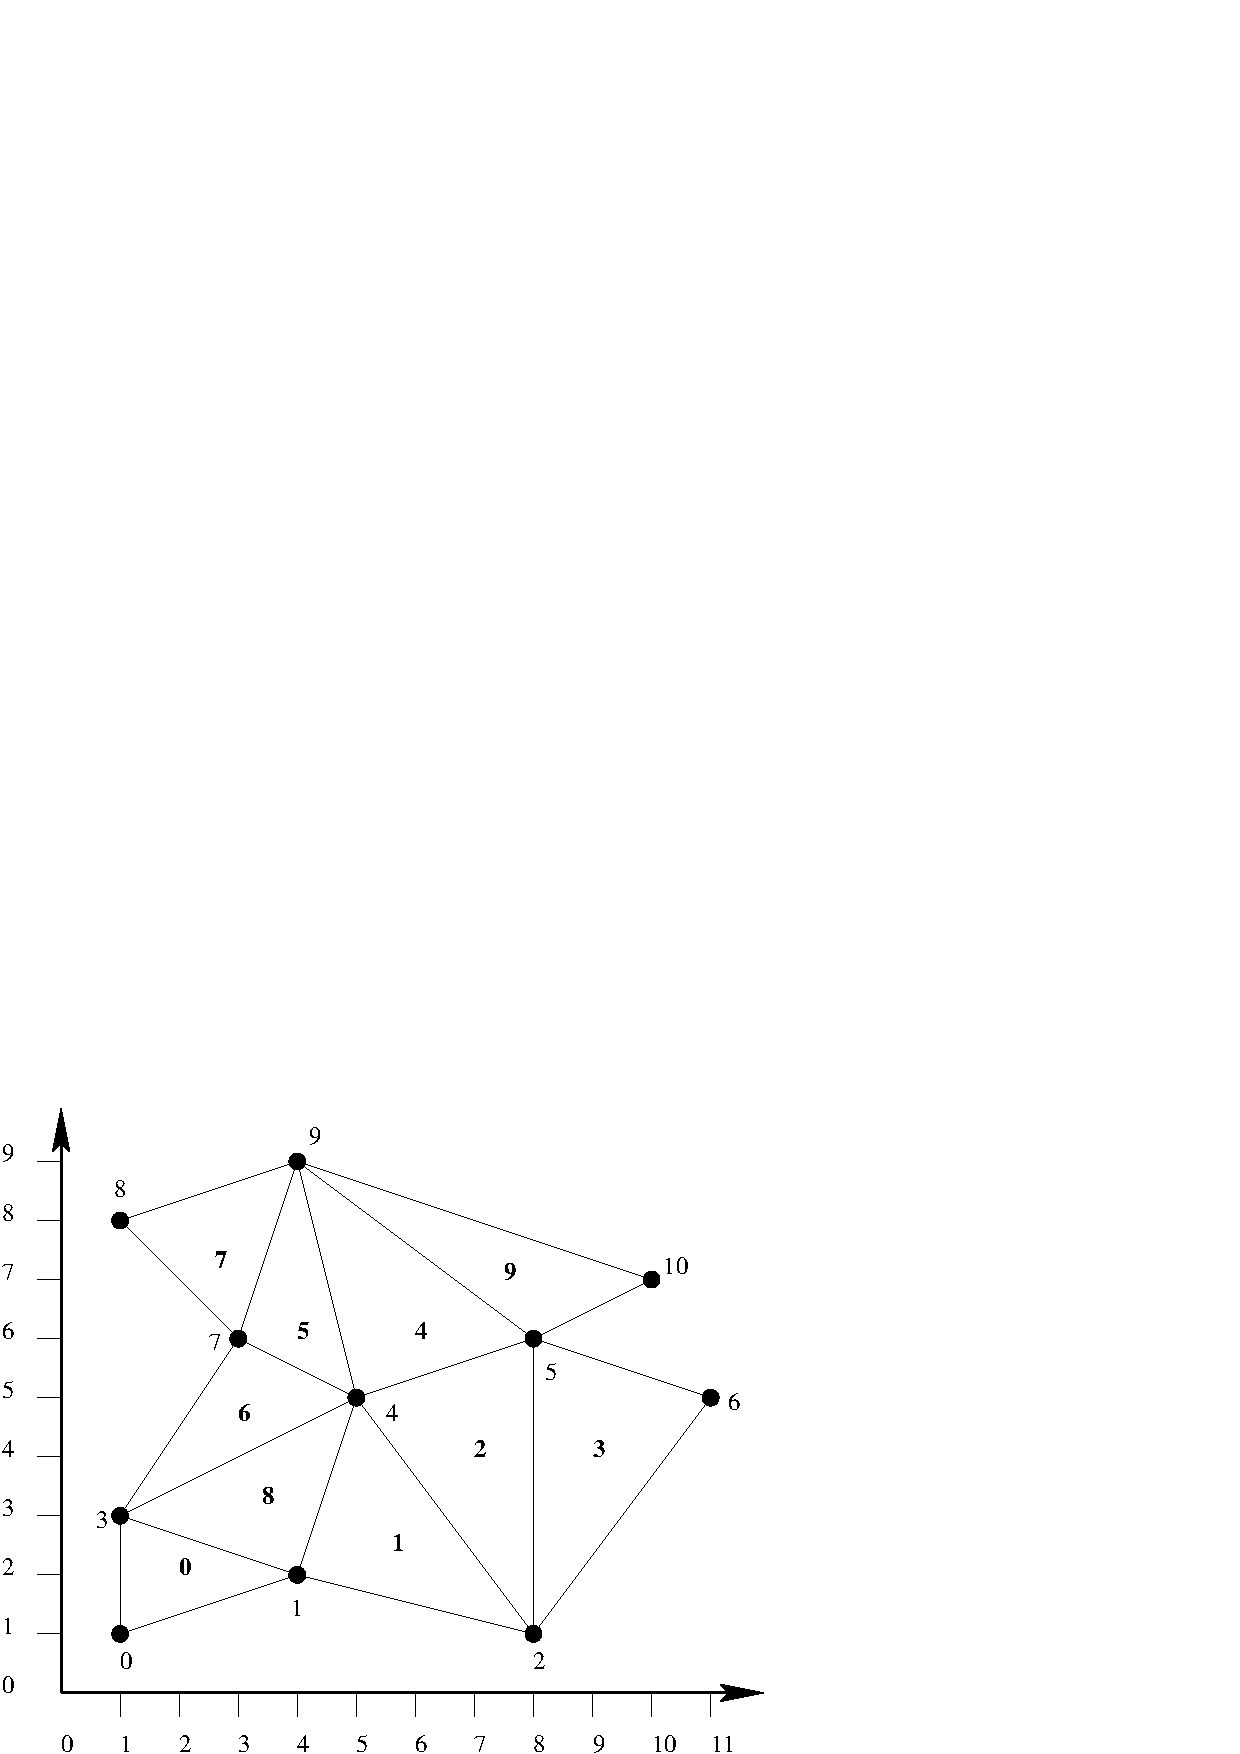
\includegraphics[width=90mm, height=90mm]{graphics/triangularmesh.jpg}
  \end{center}
  \caption{A simple mesh}
  \label{fig:simplemesh}
\end{figure}

\clearpage

The variables \code{points}, \code{triangles} and \code{boundary}
represent the data displayed in Figure \ref{fig:simplemesh} as
follows. The list \code{points} stores the coordinates of the
points, and may be displayed schematically as in Table \ref{tab:points}.

\begin{table}[htp]
  \begin{center}
    \begin{tabular}[t]{|c|cc|} \hline
      index & \code{x} & \code{y}\\  \hline
      0 & 1 & 1\\
      1 & 4 & 2\\
      2 & 8 & 1\\
      3 & 1 & 3\\
      4 & 5 & 5\\
      5 & 8 & 6\\
      6 & 11 & 5\\
      7 & 3 & 6\\
      8 & 1 & 8\\
      9 & 4 & 9\\
      10 & 10 & 7\\  \hline
    \end{tabular}
  \end{center}
  \caption{Point coordinates for mesh in Figure \protect \ref{fig:simplemesh}}
  \label{tab:points}
\end{table}

The list \code{triangles} specifies the triangles that make up the
mesh. It does this by specifying, for each triangle, the indices
(the numbers shown in the first column above) that correspond to the
three points at the triangles vertices, taken in an anti-clockwise order
around the triangle. Thus, in the example shown in Figure
\ref{fig:simplemesh}, the variable \code{triangles} contains the
entries shown in Table \ref{tab:triangles}. The starting point is
arbitrary so triangle $(0,1,3)$ is considered the same as $(1,3,0)$
and $(3,0,1)$.

\begin{table}[htp]
  \begin{center}
    \begin{tabular}{|c|ccc|}
      \hline
      index & \multicolumn{3}{c|}{\code{points}}\\
      \hline
      0 & 0 & 1 & 3\\
      1 & 1 & 2 & 4\\
      2 & 2 & 5 & 4\\
      3 & 2 & 6 & 5\\
      4 & 4 & 5 & 9\\
      5 & 4 & 9 & 7\\
      6 & 3 & 4 & 7\\
      7 & 7 & 9 & 8\\
      8 & 1 & 4 & 3\\
      9 & 5 & 10 & 9\\
      \hline
    \end{tabular}
  \end{center}

  \caption{Triangles for mesh in Figure \protect \ref{fig:simplemesh}}
  \label{tab:triangles}
\end{table}

Finally, the variable \code{boundary} identifies the boundary
triangles and associates a tag with each.

% \refmodindex[pmesh.meshinterface]{pmesh.mesh\_interface}
\label{sec:meshgeneration}

\begin{funcdesc}{create_mesh_from_regions}{bounding_polygon,
                                             boundary_tags,
                                             maximum_triangle_area=None,
                                             filename=None,
                                             interior_regions=None,
                                             interior_holes=None,
                                             hole_tags=None,
                                             poly_geo_reference=None,
                                             mesh_geo_reference=None,
                                             minimum_triangle_angle=28.0,
                                             fail_if_polygons_outside=True,
                                             breaklines=None,
                                             use_cache=False,
                                             verbose=True}
Module: \module{pmesh.mesh\_interface}

This function allows a user to initiate the automatic creation of a
mesh inside a specified polygon (input \code{bounding_polygon}).
Among the parameters that can be set are the \emph{resolution}
(maximal area for any triangle in the mesh) and the minimal angle
allowable in any triangle. The user can specify a number of internal
polygons within each of which the resolution of the mesh can be
specified. \code{interior_regions} is a paired list containing the
interior polygon and its resolution.  Additionally, the user specifies
a list of boundary tags, one for each edge of the bounding polygon.

\code{breaklines} lets you force a split along a boundary within the mesh. For
example, a kerb or the edge of a dyke could be specified here. (new in 1.2)

\code{interior_holes} lets you specify polygons as empty holes in the mesh.
This can be used  to represent buildings, pylons and other immovable
structures. These polygons do not need to be closed, but their points must be
specified in a counter-clockwise order.(new in 1.2)

\textbf{WARNING}. Note that the dictionary structure used for the
parameter \code{boundary\_tags} is different from that used for the
variable \code{boundary} that occurs in the specification of a mesh.
In the case of \code{boundary}, the tags are the \emph{values} of
the dictionary, whereas in the case of \code{boundary_tags}, the
tags are the \emph{keys} and the \emph{value} corresponding to a
particular tag is a list of numbers identifying boundary edges
labelled with that tag. Because of this, it is theoretically
possible to assign the same edge to more than one tag. However, an
attempt to do this will cause an error.

\textbf{WARNING}. Do not have polygon lines cross or be on-top of each
    other. This can result in regions of unspecified resolutions, and \anuga
    will give you an error. Do
    not have polygon close to each other. This can result in the area
    between the polygons having small triangles.  For more control
    over the mesh outline use the methods described below.

\end{funcdesc}

\begin{funcdesc}{create_domain_from_regions}{bounding_polygon,
                                             boundary_tags,
                                             maximum_triangle_area=None,
                                             mesh_filename=None,
                                             interior_regions=None,
                                             interior_holes=None,
                                             poly_geo_reference=None,
                                             mesh_geo_reference=None,
                                             minimum_triangle_angle=28.0,
                                             fail_if_polygons_outside=True,
                                             use_cache=False,
                                             verbose=True}

Module: \module{interface.py}

This higher-level function allows a user to create a domain (and associated mesh)
inside a specified polygon.

\code{bounding_polygon} is a list of points in Eastings and Northings,
relative to the zone stated in \code{poly_geo_reference} if specified.
Otherwise points are just x, y coordinates with no particular
association to any location.

\code{boundary_tags} is a dictionary of symbolic tags. For every tag there
is a list of indices referring to segments associated with that tag.
If a segment is omitted it will be assigned the default tag ''.

\code{maximum_triangle_area} is the maximal area per triangle
for the bounding polygon, excluding the interior regions.

\code{interior_holes} lets you specify polygons as empty holes in the mesh.
This can be used  to represent buildings, pylons and other immovable
structures. These polygons do not need to be closed, but their points must be
specified in a counter-clockwise order.(new in 1.2)

\code{mesh_filename} is the name of the file to contain the generated 
mesh data.

\code{interior_regions} is a list of tuples consisting of (polygon,
resolution) for each region to be separately refined. Do not have
polygon lines cross or be on-top of each other.  Also do not have
polygons close to each other.

\code{poly_geo_reference} is the geo_reference of the bounding polygon and
the interior polygons.
If none, assume absolute.  Please pass one though, since absolute
references have a zone.

\code{mesh_geo_reference} is the geo_reference of the mesh to be created.
If none is given one will be automatically generated.  It will use
the lower left hand corner of  bounding_polygon (absolute)
as the x and y values for the geo_ref.

\code{minimum_triangle_angle} is the minimum angle allowed for each generated triangle.
This controls the \emph{slimness} allowed for a triangle.

\code{fail_if_polygons_outside} -- if True (the default) an Exception in thrown
if interior polygons fall outside the bounding polygon. If False, these
will be ignored and execution continues.

\textbf{WARNING}. Note that the dictionary structure used for the
parameter \code{boundary_tags} is different from that used for the
variable \code{boundary} that occurs in the specification of a mesh.
In the case of \code{boundary}, the tags are the \emph{values} of
the dictionary, whereas in the case of \code{boundary_tags}, the
tags are the \emph{keys} and the \emph{value} corresponding to a
particular tag is a list of numbers identifying boundary edges
labelled with that tag. Because of this, it is theoretically
possible to assign the same edge to more than one tag. However, an
attempt to do this will cause an error.

\textbf{WARNING}. Do not have polygon lines cross or be on-top of each
    other. This can result in regions of unspecified resolutions. Do
    not have polygon close to each other. This can result in the area
    between the polygons having small triangles.  For more control
    over the mesh outline use the methods described below.

\end{funcdesc}

\subsection{Advanced mesh generation}

For more control over the creation of the mesh outline, use the
methods of the class \class{Mesh}.

\begin{classdesc}{Mesh}{userSegments=None,
                        userVertices=None,
                        holes=None,
                        regions=None,
                        geo_reference=None}
Module: \module{pmesh.mesh}

A class used to build a mesh outline and generate a two-dimensional
triangular mesh. The mesh outline is used to describe features on the
mesh, such as the mesh boundary. Many of this class's methods are used
to build a mesh outline, such as \code{add_vertices()} and
\code{add_region_from_polygon()}.

\code{userSegments} and \code{userVertices} define the outline enclosing the mesh.

\code{holes} describes any regions inside the mesh that are not to be included in the mesh.

\code{geo_reference} defines the geo_reference to which all point information is relative.
If \code{geo_reference} is \code{None} then the default geo_reference is used.
\end{classdesc}

\subsubsection{Key Methods of Class Mesh}

\begin{methoddesc}{\emph{<mesh>}.add_hole}{x, y, geo_reference=None}
Module: \module{pmesh.mesh}

This method adds a hole to the mesh outline.

\code{x} and \code{y} define a point on the already defined hole boundary.

If \code{geo_reference} is not supplied the points are assumed to be absolute.
\end{methoddesc}

\begin{methoddesc}{\emph{<mesh>}.add_hole_from_polygon}{polygon,
                                                        segment_tags=None,
                                                        geo_reference=None}
Module: \module{pmesh.mesh}

This method is used to add a 'hole' within a region -- that is, to
define a interior region where the triangular mesh will not be
generated -- to a \class{Mesh} instance. The region boundary is described by
the polygon passed in.  Additionally, the user specifies a list of
boundary tags, one for each edge of the bounding polygon.

\code{polygon} is the polygon that defines the hole to be added to the \code{<mesh>}.

\code{segment_tags} -- ??

If \code{geo_reference} is \code{None} then the default \code{geo_reference} is used.
\end{methoddesc}

\begin{methoddesc}{\emph{<mesh>}.add_points_and_segments}{points,
                                                          segments=None,
                                                          segment_tags=None}
Module: \module{pmesh.mesh}

This adds points and segments connecting the points to a mesh.

\code{points} is a list of points.

\code{segments} is a list of segments.  Each segment is defined by the start and end
of the line by its point index, e.g.\ use \code{segments = [[0,1],[1,2]]} to make a
polyline between points 0, 1 and 2.

\code{segment_tags} may be used to optionally define a tag for each segment.
\end{methoddesc}

\begin{methoddesc}{\emph{<mesh>}.add_region}{x,y, geo_reference=None, tag=None}
Module: \module{pmesh.mesh}

This method adds a region to a mesh outline.

\code{x} and \code{y} define a point on the already-defined region that is to 
be added to the mesh.

If \code{geo_reference} is not supplied the points data is assumed to be absolute.

\code{tag} -- ??

A region instance is returned.  This can be used to set the resolution of the added region.
\end{methoddesc}

\begin{methoddesc}{\emph{<mesh>}.add_region_from_polygon}{polygon,
                                                          segment_tags=None,
                                                          max_triangle_area=None,
                                                          geo_reference=None,
                                                          region_tag=None}
Module: \module{pmesh.mesh}

This method adds a region to a
\class{Mesh} instance.  Regions are commonly used to describe an area
with an increased density of triangles by setting \code{max_triangle_area}.

\code{polygon} describes the region boundary to add to the \code{<mesh>}.

\code{segment_tags} specifies a list of segment tags, one for each edge of the
bounding polygon.

If \code{geo_reference} is not supplied the points data is assumed to be absolute.

\code{region_tag} sets the region tag.
\end{methoddesc}

\begin{methoddesc}{\emph{<mesh>}.add_vertices}{point_data}
Module: \module{pmesh.mesh}

Add user vertices to a mesh.

\code{point_data} is the list of point data, and can be a list of (x,y) values,
a numeric array or a geospatial_data instance.
\end{methoddesc}

\begin{methoddesc}{\emph{<mesh>}.auto_segment}{alpha=None,
                                               raw_boundary=True,
                                               remove_holes=False,
                                               smooth_indents=False,
                                               expand_pinch=False}
Module: \module{pmesh.mesh}

Add segments between some of the user vertices to give the vertices an
outline.  The outline is an alpha shape. This method is
useful since a set of user vertices need to be outlined by segments
before generate_mesh is called.

\code{alpha} determines the $smoothness$ of the alpha shape.

\code{raw_boundary}, if \code{True} instructs the function to return the raw
boundary, i.e.\ the regular edges of the alpha shape.

\code{remove_holes}, if \code{True} enables a filter to remove small holes
(small is defined by  boundary_points_fraction).

\code{smooth_indents}, if \code{True} removes sharp triangular indents
in the boundary.

\code{expand_pinch}, if \code{True} tests for pinch-off and corrects
(i.e.\ a boundary vertex with more than two edges).
\end{methoddesc}

\begin{methoddesc}{\emph{<mesh>}.export_mesh_file}{ofile}
Module: \module{pmesh.mesh}

This method is used to save a mesh to a file.

\code{ofile} is the name of the mesh file to be written, including the extension.
Use the extension \code{.msh} for the file to be in NetCDF format and
\code{.tsh} for the file to be ASCII format.
\end{methoddesc}

\begin{methoddesc}{\emph{<mesh>}.generate_mesh}{maximum_triangle_area="",
                                                minimum_triangle_angle=28.0,
                                                verbose=True}
Module: \module{pmesh.mesh}

This method is used to generate the triangular mesh.

\code{maximum_triangle_area} sets the maximum area of any triangle in the mesh.

\code{minimum_triangle_angle} sets the minimum area of any triangle in the mesh.

These two parameters can be used to control the triangle density.
\end{methoddesc}

\begin{methoddesc}{\emph{<mesh>}.import_ungenerate_file}{ofile,
                                                         tag=None,
                                                         region_tag=None}
Module: \module{pmesh.mesh}

This method is used to import a polygon file in the ungenerate format,
which is used by arcGIS. The polygons from the file are converted to
vertices and segments.

\code{ofile} is the name of the polygon file.

\code{tag} is the tag given to all the polygon's segments.
If \code{tag} is not supplied then the segment will not effect the water
flow, it will only effect the mesh generation.

\code{region_tag} is the tag given to all the polygon's segments.  If
it is a string the tag will be assigned to all regions.  If it
is a list the first value in the list will be applied to the first
polygon etc.

This function can be used to import building footprints.
\end{methoddesc}


\section{Initialising the Domain}\index{Initialising the Domain}
\label{sec:initialising the domain}

\begin{classdesc}{Domain}{source=None,
                          triangles=None,
                          boundary=None,
                          conserved_quantities=None,
                          other_quantities=None,
                          tagged_elements=None,
                          geo_reference=None,
                          use_inscribed_circle=False,
                          mesh_filename=None,
                          use_cache=False,
                          verbose=False,
                          full_send_dict=None,
                          ghost_recv_dict=None,
                          processor=0,
                          numproc=1,
                          number_of_full_nodes=None,
                          number_of_full_triangles=None}
Module: \refmodule{abstract_2d_finite_volumes.domain}

This class is used to create an instance of a structure used to
store and manipulate data associated with a mesh. The mesh is
specified either by assigning the name of a mesh file to
\code{source} or by specifying the points, triangle and boundary of the
mesh.
\end{classdesc}

\subsection{Key Methods of Domain}

\begin{methoddesc}{\emph{<domain>}.set_name}{name}
Module: \refmodule{abstract_2d_finite_volumes.domain},
page \pageref{mod:domain}

\code{name} is used to name the domain.  The \code{name} is also used to identify the output SWW file.
If no name is assigned to a domain, the assumed name is \code{'domain'}.
\end{methoddesc}

\begin{methoddesc}{\emph{<domain>}.get_name}{}
Module: \module{abstract_2d_finite_volumes.domain}

Returns the name assigned to the domain by \code{set_name()}. If no name has been
assigned, returns \code{'domain'}.
\end{methoddesc}

\begin{methoddesc}{\emph{<domain>}.set_datadir}{path}
Module: \module{abstract_2d_finite_volumes.domain}

\code{path} specifies the path to the directory used to store SWW files.

Before this method is used to set the SWW directory path, the assumed directory
path is \code{default_datadir} specified in \code{config.py}.

Since different operating systems use different formats for specifying pathnames
it is necessary to specify path separators using the Python code \code{os.sep} rather than
the operating-specific ones such as '$\slash$' or '$\backslash$'.
For this to work you will need to include the statement \code{import os}
in your code, before the first use of \code{set_datadir()}.

For example, to set the data directory to a subdirectory
\code{data} of the directory \code{project}, you could use
the statements:

\begin{verbatim}
import os
domain.set_datadir{'project' + os.sep + 'data'}
\end{verbatim}
\end{methoddesc}

\begin{methoddesc}{\emph{<domain>}.get_datadir}{}
Module: \module{abstract_2d_finite_volumes.domain}

Returns the path to the directory where SWW files will be stored.

If the path has not previously been set with \code{set_datadir()} this method
will return the value \code{default_datadir} specified in \code{config.py}.
\end{methoddesc}

\begin{methoddesc}{\emph{<domain>}.set_minimum_allowed_height}{minimum_allowed_height}
Module: \module{shallow_water.shallow_water_domain}

Set the minimum depth (in metres) that will be recognised in
the numerical scheme (including limiters and flux computations)

\code{minimum_allowed_height} is the new minimum allowed height value.

Default value is $10^{-3}$ metre, but by setting this to a greater value,
e.g.\ for large scale simulations, the computation time can be
significantly reduced.
\end{methoddesc}

\begin{methoddesc}{\emph{<domain>}.set_minimum_storable_height}{minimum_storable_height}
Module: \module{shallow_water.shallow_water_domain}

Sets the minimum depth that will be recognised when writing
to an SWW file. This is useful for removing thin water layers
that seems to be caused by friction creep.

\code{minimum_storable_height} is the new minimum storable height value.
\end{methoddesc}

\begin{methoddesc}{\emph{<domain>}.set_maximum_allowed_speed}{maximum_allowed_speed}
Module: \module{shallow_water.shallow_water_domain}

Set the maximum particle speed that is allowed in water
shallower than \code{minimum_allowed_height}. This is useful for
controlling speeds in very thin layers of water and at the same time
allow some movement avoiding pooling of water.

\code{maximum_allowed_speed} sets the maximum allowed speed value.
\end{methoddesc}

\begin{methoddesc}{\emph{<domain>}.set_time}{time=0.0}
Module: \module{abstract_2d_finite_volumes.domain}

\code{time} sets the initial time, in seconds, for the simulation. The
default is 0.0.
\end{methoddesc}

\begin{methoddesc}{\emph{<domain>}.set_default_order}{n}
Module: \module{abstract_2d_finite_volumes.domain}

Sets the default (spatial) order to the value specified by
\code{n}, which must be either 1 or 2. (Assigning any other value
to \code{n} will cause an error.)
\end{methoddesc}

\begin{methoddesc}{\emph{<domain>}.set_store_vertices_uniquely}{flag, reduction=None}
Module: \module{shallow_water.shallow_water_domain}

Decide whether vertex values should be stored uniquely as
computed in the model or whether they should be reduced to one
value per vertex using averaging.

\code{flag} may be \code{True} (meaning allow surface to be discontinuous) or \code{False} (meaning smooth vertex values).

\code{reduction} defines the smoothing operation if \code{flag} is \code{False}.  If not
supplied, \code{reduction} is assumed to be \code{mean}.

Triangles stored in the SWW file can be discontinuous reflecting
the internal representation of the finite-volume scheme
(this is a feature allowing for arbitrary steepness of the water surface gradient
as well as the momentum gradients).
However, for visual purposes and also for use with \code{Field_boundary}
(and \code{File_boundary}), it is often desirable to store triangles
with values at each vertex point as the average of the potentially
discontinuous numbers found at vertices of different triangles sharing the
same vertex location.

Storing one way or the other is controlled in \anuga through the method
\code{<domain>.store_vertices_uniquely()}. Options are:
\begin{itemize}
  \item \code{<domain>.store_vertices_uniquely(True)}: Allow discontinuities in the SWW file
  \item \code{<domain>.store_vertices_uniquely(False)}: (Default).
  Average values
  to ensure continuity in SWW file. The latter also makes for smaller
  SWW files.
\end{itemize}

Note that when model data in the SWW file are averaged (i.e.\ not stored uniquely), 
then there will most likely be a small discrepancy between values extracted from the SWW 
file and the same data stored in the model domain. This must be borne in mind when comparing
data from the SWW files with that of the model internally. 
\end{methoddesc}


\begin{methoddesc}{\emph{<domain>}.set_quantities_to_be_stored}{quantity_dictionary}
Module: \module{shallow_water.shallow_water_domain}

Selects quantities that is to be stored in the sww files.
The argument can be None, in which case nothing is stored.

Otherwise, the argument must be a dictionary where the keys are names of quantities 
already defined within ANUGA and the values are either 1 or 2. If the value is 1, the quantity 
will be stored once at the beginning of the simulation, if the value is 2 it will be stored 
at each timestep. The ANUGA default is equivalent to the call
\begin{verbatim} 
domain.set_quantities_to_be_stored({'elevation': 1,
                                    'stage': 2, 
                                    'xmomentum': 2, 
                                    'ymomentum': 2})
\end{verbatim} 
\end{methoddesc}


% Structural methods
\begin{methoddesc}{\emph{<domain>}.get_nodes}{absolute=False}
Module: \module{abstract_2d_finite_volumes.domain}

Return x,y coordinates of all nodes in the domain mesh.  The nodes are ordered
in an \code{Nx2} array where N is the number of nodes.  This is the same format
they were provided in the constructor i.e.\ without any duplication.

\code{absolute} is a boolean which determines whether coordinates
are to be made absolute by taking georeference into account.
Default is \code{False} as many parts of \anuga expect relative coordinates.
\end{methoddesc}

\begin{methoddesc}{\emph{<domain>}.get_vertex_coordinates}{absolute=False}
Module: \module{abstract_2d_finite_volumes.domain}

\label{pg:get vertex coordinates}
Return vertex coordinates for all triangles as a \code{3*Mx2} array
where the jth vertex of the ith triangle is located in row 3*i+j and
M is the number of triangles in the mesh.

\code{absolute} is a boolean which determines whether coordinates
are to be made absolute by taking georeference into account.
Default is \code{False} as many parts of \anuga expect relative coordinates.
\end{methoddesc}

\begin{methoddesc}{\emph{<domain>}.get_centroid_coordinates}{absolute=False}
Module: \module{abstract_2d_finite_volumes.domain}

Return centroid coordinates for all triangles as an \code{Mx2} array.
    
\code{absolute} is a boolean which determines whether coordinates
are to be made absolute by taking georeference into account.
Default is \code{False} as many parts of \anuga expect relative coordinates.
\end{methoddesc}

\begin{methoddesc}{\emph{<domain>}.get_triangles}{indices=None}
Module: \module{abstract_2d_finite_volumes.domain}

Return an \code{Mx3} integer array where M is the number of triangles.
Each row corresponds to one triangle and the three entries are
indices into the mesh nodes which can be obtained using the method
\code{get_nodes()}.

\code{indices}, if specified, is the set of triangle \code{id}s of interest.
\end{methoddesc}

\begin{methoddesc}{\emph{<domain>}.get_disconnected_triangles}{}
Module: \module{abstract_2d_finite_volumes.domain}

Get the domain mesh based on nodes obtained from \code{get_vertex_coordinates()}.

Returns an \code{Mx3} array of integers where each row corresponds to
a triangle. A triangle is a triplet of indices into
point coordinates obtained from \code{get_vertex_coordinates()} and each
index appears only once.

This provides a mesh where no triangles share nodes
(hence the name disconnected triangles) and different
nodes may have the same coordinates.

This version of the mesh is useful for storing meshes with
discontinuities at each node and is e.g.\ used for storing
data in SWW files.

The triangles created will have the format:

\begin{verbatim}
[[0,1,2],
 [3,4,5],
 [6,7,8],
 ...
 [3*M-3 3*M-2 3*M-1]]
\end{verbatim}
\end{methoddesc}


\section{Initial Conditions}\index{Initial Conditions}
\label{sec:initial conditions}
In standard usage of partial differential equations, initial conditions
refers to the values associated to the system variables (the conserved
quantities here) for \code{time = 0}. In setting up a scenario script
as described in Sections \ref{sec:simpleexample} and \ref{sec:realdataexample},
\code{set_quantity} is used to define the initial conditions of variables
other than the conserved quantities, such as friction. Here, we use the terminology
of initial conditions to refer to initial values for variables which need
prescription to solve the shallow water wave equation. Further, it must be noted
that \code{set_quantity()} does not necessarily have to be used in the initial
condition setting; it can be used at any time throughout the simulation.

\begin{methoddesc}{\emph{<domain>}.set_quantity}{numeric=None,
                                                 quantity=None,
                                                 function=None,
                                                 geospatial_data=None,
                                                 filename=None,
                                                 attribute_name=None,
                                                 alpha=None,
                                                 location='vertices',
                                                 polygon=None,
                                                 indices=None,
                                                 smooth=False,
                                                 verbose=False,
                                                 use_cache=False}
Module: \module{abstract_2d_finite_volumes.domain} \\
(This method passes off to \module{abstract_2d_finite_volumes.quantity.set_values()})

This function is used to assign values to individual quantities for a
domain. It is very flexible and can be used with many data types: a
statement of the form \code{\emph{<domain>}.set_quantity(name, x)} can be used
to define a quantity having the name \code{name}, where the other
argument \code{x} can be any of the following:

\begin{itemize}
  \item a number, in which case all vertices in the mesh gets that for
        the quantity in question
  \item a list of numbers or a numeric array ordered the same way as the mesh vertices
  \item a function (e.g.\ see the samples introduced in Chapter 2)
  \item an expression composed of other quantities and numbers, arrays, lists (for
        example, a linear combination of quantities, such as
        \code{\emph{<domain>}.set_quantity('stage','elevation'+x))}
  \item the name of a file from which the data can be read. In this case, the optional
        argument \code{attribute_name} will select which attribute to use from the file. If left out,
        \code{set_quantity()} will pick one. This is useful in cases where there is only one attribute
  \item a geospatial dataset (See Section \ref{sec:geospatial}).
        Optional argument \code{attribute_name} applies here as with files
\end{itemize}

Exactly one of the arguments \code{numeric}, \code{quantity}, \code{function},
\code{geospatial_data} and \code{filename} must be present.

\code{set_quantity()} will look at the type of the \code{numeric} and
determine what action to take.

Values can also be set using the appropriate keyword arguments.
If \code{x} is a function, for example, \code{domain.set_quantity(name, x)}, \code{domain.set_quantity(name, numeric=x)},
and \code{domain.set_quantity(name, function=x)} are all equivalent.

Other optional arguments are:
\begin{itemize}
  \item \code{indices} which is a list of ids of triangles to which \code{set_quantity()}
        should apply its assignment of values.
  \item \code{location} determines which part of the triangles to assign to.
        Options are 'vertices' (the default), 'edges', 'unique vertices', and 'centroids'.
        If 'vertices' is used, edge and centroid values are automatically computed as the
        appropriate averages. This option ensures continuity of the surface.
        If, on the other hand, 'centroids' is used, vertex and edge values will be set to the
        same value effectively creating a piecewise constant surface with possible
        discontinuities at the edges.
\end{itemize}

\anuga provides a number of predefined initial conditions to be used
with \code{set_quantity()}. See for example callable object \code{slump_tsunami} below.
\end{methoddesc}

\begin{methoddesc}{\emph{<domain>}.add_quantity}{numeric=None,
                                                 quantity=None,
                                                 function=None,
                                                 geospatial_data=None,
                                                 filename=None,
                                                 attribute_name=None,
                                                 alpha=None,
                                                 location='vertices',
                                                 polygon=None,
                                                 indices=None,
                                                 smooth=False,
                                                 verbose=False,
                                                 use_cache=False}
Module: \module{abstract_2d_finite_volumes.domain} \\
(passes off to \module{abstract_2d_finite_volumes.domain.set_quantity()})

\label{add quantity}
This function is used to \emph{add} values to individual quantities for a
domain. It has the same syntax as \code{\emph{<domain>}.set_quantity(name, x)}.

A typical use of this function is to add structures to an existing elevation model:

\begin{verbatim} 
# Create digital elevation model from points file
domain.set_quantity('elevation', filename='elevation_file.pts, verbose=True)

# Add buildings from file
building_polygons, building_heights = anuga.load_csv_as_building_polygons(building_file)

B = []
for key in building_polygons:
    poly = building_polygons[key]
    elev = building_heights[key]
    B.append((poly, elev))

domain.add_quantity('elevation', Polygon_function(B, default=0.0))
\end{verbatim}
\end{methoddesc}

\begin{methoddesc}{\emph{<domain>}.set_region}{tag, quantity, X, location='vertices'}
Module: \module{abstract_2d_finite_volumes.domain} \\
(see also \module{abstract_2d_finite_volumes.quantity.set_values})

This function is used to assign values to individual quantities given
a regional tag.   It is similar to \code{set_quantity()}.

For example, if in the mesh-generator a regional tag of 'ditch' was
used, \code{set_region()} can be used to set elevation of this region to
-10m. \code{X} is the constant or function to be applied to the \code{quantity},
over the tagged region.  \code{location} describes how the values will be
applied.  Options are 'vertices' (the default), 'edges', 'unique
vertices', and 'centroids'.

This method can also be called with a list of region objects.  This is
useful for adding quantities in regions, and having one quantity
value based on another quantity. See  \module{abstract_2d_finite_volumes.region} for
more details.
\end{methoddesc}

\begin{funcdesc}{slump_tsunami}{length, depth, slope, width=None, thickness=None,
                                radius=None, dphi=0.48, x0=0.0, y0=0.0, alpha=0.0,
                                gravity=9.8, gamma=1.85,
                                massco=1, dragco=1, frictionco=0,
                                dx=None, kappa=3.0, kappad=1.0, zsmall=0.01, scale=None,
                                domain=None,
                                verbose=False}
Module: \module{shallow\_water.smf}

This function returns a callable object representing an initial water
displacement generated by a submarine sediment failure. These failures can take the form of
a submarine slump or slide. In the case of a slide, use \code{slide_tsunami} instead.

\code{length} is the length of the slide or slump.

\code{depth} is the water depth to the centre of the sediment mass.

\code{slope} is the bathymetric slope.

Other slump or slide parameters can be included if they are known.
\end{funcdesc}

\begin{funcdesc}{\emph{<callable_object>} = file_function}{filename,
                                domain=None,
                                quantities=None,
                                interpolation_points=None,
                                time_thinning=1,
                                time_limit=None,
                                verbose=False,
                                output_centroids=False,
                                use_cache=False,
                                boundary_polygon=None}
Module: \module{abstract_2d_finite_volumes.util}

Reads the time history of spatial data for specified interpolation points from
a NetCDF file and returns a callable object.  Values returned from the \code{\emph{<callable_object>}}
are interpolated values based on the input file using the underlying \code{interpolation_function}.

\code{filename} is the name of the input file.  
This would be either an SWW, TMS or STS file.

\code{quantities} is either the name of a single quantity to be
interpolated or a list of such quantity names. In the second case, the resulting
function will return a tuple of values -- one for each quantity.
If the NetCDF file uses names other than 'stage', 'xmomentum', and 'ymomentum'
the name(s) appearing in the file must be explicitly stated using the 
quantities keyword. This is for example be the case if a 'tms' file is used 
to specify time dependent precipitation. In this case the keyword might be called 'rainfall' both in the call to file\_function and in the 'tms' file.

\code{interpolation_points} is a list of absolute coordinates or a
geospatial object for points at which values are sought.

\code{boundary_polygon} is a list of coordinates specifying the vertices of the boundary.
This must be the same polygon as used when calling \code{create_mesh_from_regions()}.
This argument can only be used when reading boundary data from an STS format file.

\code{output_centroids} set to true to sample at the centre of the triangle containing the point.
This may be useful for debugging. (new in 1.2)

The model time stored within the file function can be accessed using
the method \code{\emph{<callable_object>}.get_time()}

The underlying algorithm used is as follows:\\
Given a time series (i.e.\ a series of values associated with
different times), whose values are either just numbers, a set of
numbers defined at the vertices of a triangular mesh (such as those
stored in SWW files) or a set of
numbers defined at a number of points on the boundary (such as those
stored in STS files), \code{Interpolation_function()} is used to
create a callable object that interpolates a value for an arbitrary
time \code{t} within the model limits and possibly a point \code{(x, y)}
within a mesh region.

The actual time series at which data is available is specified by
means of an array \code{time} of monotonically increasing times. The
quantities containing the values to be interpolated are specified in
an array -- or dictionary of arrays (used in conjunction with the
optional argument \code{quantity_names}) -- called
\code{quantities}. The optional arguments \code{vertex_coordinates}
and \code{triangles} represent the spatial mesh associated with the
quantity arrays. If omitted the function must be created using an STS file
or a TMS file.

Since, in practice, values need to be computed at specified points,
the syntax allows the user to specify, once and for all, a list
\code{interpolation_points} of points at which values are required.
In this case, the function may be called using the form \code{\emph{<callable_object>}(t, id)},
where \code{id} is an index for the list \code{interpolation_points}.
\end{funcdesc}

\begin{classdesc}{\emph{<callable_object>} = Interpolation_function}{time,
                                          quantities,
                                          quantity_names=None,
                                          vertex_coordinates=None,
                                          triangles=None,
                                          interpolation_points=None,
                                          time_thinning=1,
                                          verbose=False,
                                          gauge_neighbour_id=None}
Module: \module{fit_interpolate.interpolate}

Given a time series (i.e.\ a series of values associated with
different times) whose values are either just numbers or a set of
numbers defined at the vertices of a triangular mesh (such as those
stored in SWW files), \code{Interpolation_function} is used to
create a callable object that interpolates a value for an arbitrary
time \code{t} within the model limits and possibly a point \code{(x, y)}
within a mesh region.

The actual time series at which data is available is specified by
means of an array \code{time} of monotonically increasing times. The
quantities containing the values to be interpolated are specified in
an array -- or dictionary of arrays (used in conjunction with the
optional argument \code{quantity\_names}) -- called
\code{quantities}. The optional arguments \code{vertex_coordinates}
and \code{triangles} represent the spatial mesh associated with the
quantity arrays. If omitted the function created by
\code{Interpolation_function} will be a function of \code{t} only.

Since, in practice, values need to be computed at specified points,
the syntax allows the user to specify, once and for all, a list
\code{interpolation_points} of points at which values are required.
In this case, the function may be called using the form \code{f(t, id)},
where \code{id} is an index for the list \code{interpolation_points}.
\end{classdesc}


\section{Boundary Conditions}\index{boundary conditions}
\label{sec:boundary conditions}

\anuga provides a large number of predefined boundary conditions,
represented by objects such as \code{Reflective_boundary(domain)} and
\code{Dirichlet_boundary([0.2, 0.0, 0.0])}, described in the examples
in Chapter 2. Alternatively, you may prefer to ''roll your own'',
following the method explained in Section \ref{sec:roll your own}.

These boundary objects may be used with the function \code{set_boundary} described below
to assign boundary conditions according to the tags used to label boundary segments.

\begin{methoddesc}{\emph{<domain>}.set_boundary}{boundary_map}
Module: \module{abstract_2d_finite_volumes.domain}

This function allows you to assign a boundary object (corresponding to a
pre-defined or user-specified boundary condition) to every boundary segment that
has been assigned a particular tag.

\code{boundary_map} is a dictionary of boundary objects keyed by symbolic tags.
\end{methoddesc}

\begin{methoddesc} {\emph{<domain>}.get_boundary_tags}{}
Module: \module{abstract\_2d\_finite\_volumes.domain}

Returns a list of the available boundary tags.
\end{methoddesc}

\subsection{Predefined boundary conditions}

\begin{classdesc}{Reflective_boundary}{domain=None}
Module: \module{shallow_water}

Reflective boundary returns same conserved quantities as those present in
the neighbouring volume but reflected.

This class is specific to the shallow water equation as it works with the
momentum quantities assumed to be the second and third conserved quantities.
\end{classdesc}

\begin{classdesc}{Transmissive_boundary}{domain=None}
  \label{pg: transmissive boundary}
Module: \module{abstract_2d_finite_volumes.generic_boundary_conditions}

A transmissive boundary returns the same conserved quantities as
those present in the neighbouring volume.

The underlying domain must be specified when the boundary is instantiated.
\end{classdesc}

\begin{classdesc}{Dirichlet_boundary}{conserved_quantities=None}
Module: \module{abstract_2d_finite_volumes.generic_boundary_conditions}

A Dirichlet boundary returns constant values for each of conserved
quantities. In the example of \code{Dirichlet_boundary([0.2, 0.0, 0.0])},
the \code{stage} value at the boundary is 0.2 and the \code{xmomentum} and
\code{ymomentum} at the boundary are set to 0.0. The list must contain
a value for each conserved quantity.
\end{classdesc}

\begin{classdesc}{Time_boundary}{domain=None,
                                 function=None,
                                 default_boundary=None,
                                 verbose=False}
Module: \module{abstract_2d_finite_volumes.generic_boundary_conditions}

A time-dependent boundary returns values for the conserved
quantities as a function of time \code{function(t)}. The user must specify
the domain to get access to the model time.

Optional argument \code{default_boundary} can be used to specify another boundary object
to be used in case model time exceeds the time available in the file used by \code{File_boundary}.
The \code{default_boundary} could be a simple Dirichlet condition or
even another \code{Time_boundary} typically using data pertaining to another time interval.
\end{classdesc}

\begin{classdesc}{File_boundary}{filename,
                                 domain,
                                 time_thinning=1,
                                 time_limit=None,
                                 boundary_polygon=None,
                                 default_boundary=None,
                                 use_cache=False,
                                 verbose=False}
Module: \module{abstract_2d_finite_volumes.generic_boundary_conditions}

This method may be used if the user wishes to apply a SWW file, STS file or
a time series file (TMS) to a boundary segment or segments.
The boundary values are obtained from a file and interpolated to the
appropriate segments for each conserved quantity.

Optional argument \code{default_boundary} can be used to specify another boundary object
to be used in case model time exceeds the time available in the file used by \code{File_boundary}.
The \code{default_boundary} could be a simple Dirichlet condition or
even another \code{File_boundary} typically using data pertaining to another time interval.
\end{classdesc}

\begin{classdesc}{Field_boundary}{filename,
                                  domain,
                                  mean_stage=0.0,
                                  time_thinning=1,
                                  time_limit=None,
                                  boundary_polygon=None,
                                  default_boundary=None,
                                  use_cache=False,
                                  verbose=False}
Module: \module{shallow_water.shallow_water_domain}

This method works in the same way as \code{File_boundary} except that it
allows for the value of stage to be offset by a constant specified in the
keyword argument \code{mean_stage}.

This functionality allows for models to be run for a range of tides using
the same boundary information (from STS, SWW or TMS files). The tidal value
for each run would then be specified in the keyword argument \code{mean_stage}.
If \code{mean_stage} = 0.0, \code{Field_boundary} and \code{File_boundary}
behave identically.

Note that if the optional argument \code{default_boundary} is specified
its stage value will be adjusted by \code{mean_stage} just like the values
obtained from the file.

See \code{File_boundary} for further details.
\end{classdesc}

\begin{classdesc}{Transmissive_momentum_set_stage_boundary}{domain=None,
                                                            function=None}
Module: \module{shallow_water.shallow_water_domain}
\label{pg: transmissive momentum set stage boundary}

This boundary returns the same momentum conserved quantities as
those present in its neighbour volume but sets stage as in a \code{Time_boundary}.
The underlying domain must be specified when boundary is instantiated.

This type of boundary is useful when stage is known at the boundary as a
function of time, but momenta (or speeds) aren't.

This class is specific to the shallow water equation as it works with the
momentum quantities assumed to be the second and third conserved quantities.

In some circumstances, this boundary condition may cause numerical instabilities for similar
reasons as what has been observed with the simple fully transmissive boundary condition
(see Page \pageref{pg: transmissive boundary}). 
This could for example be the case if a planar wave is reflected out through this boundary.
\end{classdesc}

\begin{classdesc}{Transmissive_stage_zero_momentum_boundary}{domain=None}
Module: \module{shallow_water}
\label{pg: transmissive stage zero momentum boundary}

This boundary returns same stage conserved quantities as
those present in its neighbour volume but sets momentum to zero.
The underlying domain must be specified when boundary is instantiated

This type of boundary is useful when stage is known at the boundary as a
function of time, but momentum should be set to zero. This is for example
the case where a boundary is needed in the ocean on the two sides perpendicular
to the coast to maintain the wave height of the incoming wave.

This class is specific to the shallow water equation as it works with the
momentum quantities assumed to be the second and third conserved quantities.

This boundary condition should not cause the numerical instabilities seen with the transmissive momentum 
boundary conditions (see Page \pageref{pg: transmissive boundary} and
Page \pageref{pg: transmissive momentum set stage boundary}).
\end{classdesc}

\begin{classdesc}{Dirichlet_discharge_boundary}{domain=None, stage0=None, wh0=None}
Module: \module{shallow_water.shallow_water_domain}

\code{stage0} sets the stage.

\code{wh0} sets momentum in the inward normal direction.
\end{classdesc}

\subsection{User-defined boundary conditions}
\label{sec:roll your own}

All boundary classes must inherit from the generic boundary class
\code{Boundary} and have a method called \code{evaluate()} which must
take as inputs \code{self}, \code{vol_id} and \code{edge_id} where \code{self} refers to the
object itself and \code{vol_id} and \code{edge_id} are integers referring to
particular edges. The method must return a list of three floating point
numbers representing values for \code{stage},
\code{xmomentum} and \code{ymomentum}, respectively.

The constructor of a particular boundary class may be used to specify
particular values or flags to be used by the \code{evaluate()} method.
Please refer to the source code for the existing boundary conditions
for examples of how to implement boundary conditions.


\section{Forcing Terms}\index{Forcing terms}
\label{sec:forcing terms}

\anuga provides a number of predefined forcing functions to be used with simulations.
Gravity and friction are always calculated using the elevation and friction quantities,
but the user may additionally add forcing terms to the list
\code{domain.forcing_terms} and have them affect the model.

Currently, predefined forcing terms are: \\
\begin{classdesc}{General_forcing}{domain,
                                  quantity_name,
                                  rate=0.0,
                                  center=None,
                                  radius=None,
                                  polygon=None,
                                  default_rate=None,
                                  verbose=False}
Module: \module{shallow_water.shallow_water_domain}

This is a general class to modify any quantity according to a given rate of change.
Other specific forcing terms are based on this class but it can be used by itself as well (e.g.\ to modify momentum).

\code{domain} is the domain being evolved.

\code{quantity_name} is the name of the quantity that will be affected by this forcing term.

\code{rate} is the rate at which the quantity should change. This can be either a constant or a
function of time. Positive values indicate increases, negative values indicate decreases.
The parameter \code{rate} can be \code{None} at initialisation but must be specified
before a forcing term is applied (i.e.\ simulation has started).
The default value is 0.0 -- i.e.\ no forcing.

\code{center} and \code{ radius} optionally restrict forcing to a circle with given center and radius.

\code{polygon} optionally restricts forcing to an area enclosed by the given polygon.

Note: specifying \code{center}, \code{radius} and \code{polygon} will cause an exception to be thrown.
Moreover, if the specified polygon or circle does not lie fully within the mesh boundary an Exception will be thrown.

Example:

\begin{verbatim}
P = [[x0, y0], [x1, y0], [x1, y1], [x0, y1]]    # Square polygon

xmom = General_forcing(domain, 'xmomentum', polygon=P)
ymom = General_forcing(domain, 'ymomentum', polygon=P)

xmom.rate = f
ymom.rate = g

domain.forcing_terms.append(xmom)
domain.forcing_terms.append(ymom)
\end{verbatim}

Here, \code{f} and \code{g} are assumed to be defined as functions of time providing
a time dependent rate of change for xmomentum and ymomentum respectively.
\code{P} is assumed to be the polygon, specified as a list of points.
\end{classdesc}

\begin{classdesc}{Inflow}{domain,
                         rate=0.0,
                         center=None, radius=None,
                         polygon=None,
                         default_rate=None,
                         verbose=False}
Module: \module{shallow_water.shallow_water_domain}

This is a general class for inflow and abstraction of water according to a given rate of change.
This class will always modify the \code{stage} quantity.

Inflow is based on the \code{General_forcing} class so the functionality is similar.

\code{domain} is the domain being evolved.

\code{rate} is the flow rate ($m^3/s$) at which the quantity should change. This can be either a constant or a
function of time. Positive values indicate inflow, negative values indicate outflow.
Note: The specified flow will be divided by the area of the inflow region and then applied to update the
stage quantity.

\code{center} and \code{ radius} optionally restrict forcing to a circle with given center and radius.

\code{polygon} optionally restricts forcing to an area enclosed by the given polygon.

Example:

\begin{verbatim}
hydrograph = Inflow(center=(320, 300), radius=10,
                    rate=file_function('QPMF_Rot_Sub13.tms'))

domain.forcing_terms.append(hydrograph)
\end{verbatim}

Here, \code{'QPMF_Rot_Sub13.tms'} is assumed to be a NetCDF file in the TMS format defining a timeseries for a hydrograph.
\end{classdesc}

\begin{classdesc}{Rainfall}{domain,
                           rate=0.0,
                           center=None,
                           radius=None,
                           polygon=None,
                           default_rate=None,
                           verbose=False}
Module: \module{shallow_water.shallow_water_domain}

This is a general class for implementing rainfall over the domain, possibly restricted to a given circle or polygon.
This class will always modify the \code{stage} quantity.

Rainfall is based on the \code{General_forcing} class so the functionality is similar.

\code{domain} is the domain being evolved.

\code{rate} is the total rain rate over the specified domain.
Note: Raingauge Data needs to reflect the time step.
For example, if rain gauge is \code{mm} read every \code{dt} seconds, then the input
here is as \code{mm/dt} so 10 mm in 5 minutes becomes
10/(5x60) = 0.0333mm/s.  This parameter can be either a constant or a
function of time. Positive values indicate rain being added (or be used for general infiltration),
negative values indicate outflow at the specified rate (presumably this could model evaporation or abstraction).

\code{center} and \code{ radius} optionally restrict forcing to a circle with given center and radius.

\code{polygon} optionally restricts forcing to an area enclosed by the given polygon.

Example:

\begin{verbatim}
catchmentrainfall = Rainfall(rate=file_function('Q100_2hr_Rain.tms'))
domain.forcing_terms.append(catchmentrainfall)
\end{verbatim}

Here, \code{'Q100_2hr_Rain.tms'} is assumed to be a NetCDF file in the TMS format defining a timeseries for the rainfall.
\end{classdesc}

\begin{classdesc}{Culvert_flow}{domain,
                 culvert_description_filename=None,
                 culvert_routine=None,
                 end_point0=None,
                 end_point1=None,
                 enquiry_point0=None,
                 enquiry_point1=None,
                 type='box',
                 width=None,
                 height=None,
                 length=None,
                 number_of_barrels=1,
                 trigger_depth=0.01,
                 manning=None,
                 sum_loss=None,
                 use_velocity_head=False,
                 use_momentum_jet=False,
                 label=None,
                 description=None,
                 update_interval=None,
                 log_file=False,
                 discharge_hydrograph=False,
                 verbose=False}
Module: \module{culvert_flows.culvert_class}

This is a general class for implementing flow through a culvert.
This class modifies the quantities \code{stage}, \code{xmomentum} and \code{ymomentum} in areas at both ends of the culvert.

The \code{Culvert_flow} forcing term uses \code{Inflow} and \code{General_forcing} to update the quantities.
The flow direction is determined on-the-fly so openings are referenced simple as opening0 and opening1
with either being able to take the role as Inflow or Outflow.

The \code{Culvert_flow} class takes as input:
\begin{itemize}
  \item \code{domain}: a reference to the domain being evolved
  \item \code{culvert_description_filename}:
  \item \code{culvert_routine}:
  \item \code{end_point0}: Coordinates of one opening
  \item \code{end_point1}: Coordinates of other opening
  \item \code{enquiry_point0}:
  \item \code{enquiry_point1}:
  \item \code{type}: (default is 'box')
  \item \code{width}:
  \item \code{height}:
  \item \code{length}:
  \item \code{number_of_barrels}: Number of identical pipes in the culvert (default is 1)
  \item \code{trigger_depth}: (default is 0.01)
  \item \code{manning}: Mannings Roughness for Culvert
  \item \code{sum_loss}:
  \item \code{use_velocity_head}:
  \item \code{use_momentum_jet}:
  \item \code{label}: Short text naming the culvert
  \item \code{description}: Text describing the culvert
  \item \code{update_interval}:
  \item \code{log_file}:
  \item \code{discharge_hydrograph}:
\end{itemize}

The user can specify different culvert routines. However, \anuga currently provides only one, namely the
\code{boyd_generalised_culvert_model} as used in the example below:

\begin{verbatim}
from anuga.culvert_flows.culvert_class import Culvert_flow
from anuga.culvert_flows.culvert_routines import boyd_generalised_culvert_model

culvert1 = Culvert_flow(domain,
                        label='Culvert No. 1',
                        description='This culvert is a test unit 1.2m Wide by 0.75m High',
                        end_point0=[9.0, 2.5],
                        end_point1=[13.0, 2.5],
                        width=1.20,
                        height=0.75,
                        culvert_routine=boyd_generalised_culvert_model,
                        number_of_barrels=1,
                        verbose=True)

culvert2 = Culvert_flow(domain,
                        label='Culvert No. 2',
                        description='This culvert is a circular test with d=1.2m',
                        end_point0=[9.0, 1.5],
                        end_point1=[30.0, 3.5],
                        diameter=1.20,
                        invert_level0=7,
                        culvert_routine=boyd_generalised_culvert_model,
                        number_of_barrels=1,
                        verbose=True)

domain.forcing_terms.append(culvert1)
domain.forcing_terms.append(culvert2)
\end{verbatim}
\end{classdesc}


\section{Evolution}\index{evolution}
\label{sec:evolution}

\begin{methoddesc}{\emph{<domain>}.evolve}{yieldstep=None,
                                           finaltime=None,
                                           duration=None,
                                           skip_initial_step=False}
Module: \module{abstract_2d_finite_volumes.domain}

This method is invoked once all the
preliminaries have been completed, and causes the model to progress
through successive steps in its evolution, storing results and
outputting statistics whenever a user-specified period
\code{yieldstep} is completed.  Generally during this period the
model will evolve through several steps internally
as the method forces the water speed to be calculated
on successive new cells. 

\code{yieldstep} is the interval in seconds between yields where results are
stored, statistics written and the domain is inspected or possibly modified.
If omitted an internal predefined \code{yieldstep} is used.  Internally, smaller
timesteps may be taken.

\code{duration} is the duration of the simulation in seconds.

\code{finaltime} is the time in seconds where simulation should end. This is currently
relative time, so it's the same as \code{duration}.  If both \code{duration} and
\code{finaltime} are given an exception is thrown.

\code{skip_initial_step} is a boolean flag that decides whether the first
yield step is skipped or not. This is useful for example to avoid
duplicate steps when multiple evolve processes are dove tailed.

The code specified by the user in the block following the evolve statement is
only executed once every \code{yieldstep} even though 
\anuga typically will take many more internal steps behind the scenes.

You can include \method{evolve} in a statement of the type:

\begin{verbatim}
for t in domain.evolve(yieldstep, finaltime):
    <Do something with domain and t>
\end{verbatim}
\end{methoddesc}

\subsection{Diagnostics}
\label{sec:diagnostics}

\begin{methoddesc}{\emph{<domain>}.statistics}{}
Module: \module{abstract\_2d\_finite\_volumes.domain}

Outputs statistics about the mesh within the \code{Domain}.
\end{methoddesc}

\begin{methoddesc}{\emph{<domain>}.timestepping_statistics}{track_speeds=False, triangle_id=None}
Module: \module{abstract_2d_finite_volumes.domain}

Returns a string of the following type for each timestep:\\
\code{Time = 0.9000, delta t in [0.00598964, 0.01177388], steps=12 (12)}

Here the numbers in \code{steps=12 (12)} indicate the number of steps taken and
the number of first-order steps, respectively.

The optional keyword argument \code{track_speeds} will
generate a histogram of speeds generated by each triangle if set to \code{True}. The
speeds relate to the size of the timesteps used by \anuga and
this diagnostics may help pinpoint problem areas where excessive speeds
are generated.

The optional keyword argument \code{triangle_id} can be used to specify a particular
triangle rather than the one with the largest speed.
\end{methoddesc}

\begin{methoddesc}{\emph{<domain>}.boundary_statistics}{quantities=None,
                                                      tags=None}
Module: \module{abstract_2d_finite_volumes.domain}

Generates output about boundary forcing at each timestep.

\code{quantities} names the quantities to be reported -- may be \code{None},
a string or a list of strings.

\code{tags} names the tags to be reported -- may be either None, a string or a list of strings.

When \code{quantities = 'stage'} and \code{tags = ['top', 'bottom']}
will return a string like:

\begin{verbatim}
Boundary values at time 0.5000:
    top:
        stage in [ -0.25821218,  -0.02499998]
    bottom:
        stage in [ -0.27098821,  -0.02499974]
\end{verbatim}
\end{methoddesc}

\begin{methoddesc}{Q = \emph{<domain>}.get_quantity}{name,
                                               location='vertices',
                                               indices=None}
Module: \module{abstract_2d_finite_volumes.domain}

This function returns a Quantity object Q.
Access to its values should be done through \code{Q.get_values()} documented on Page \pageref{pg:get values}.

\code{name} is the name of the quantity to retrieve.

\code{location} is

\code{indices} is
\end{methoddesc}

\begin{methoddesc}{\emph{<domain>}.set_quantities_to_be_monitored}{quantity,
                                             polygon=None,
                                             time_interval=None}
Module: \module{abstract\_2d\_finite\_volumes.domain}

Selects quantities and derived quantities for which extrema attained at internal timesteps
will be collected.

\code{quantity} specifies the quantity or quantities to be monitored and must be either:
\begin{itemize}
  \item the name of a quantity or derived quantity such as 'stage-elevation',
  \item a list of quantity names, or
  \item \code{None}.
\end{itemize}

\code{polygon} can be used to monitor only triangles inside the polygon. Otherwise
all triangles will be included.

\code{time_interval} will restrict monitoring to time steps in the interval. Otherwise
all timesteps will be included.

Information can be tracked in the evolve loop by printing \code{quantity_statistics} and
collected data will be stored in the SWW file.
\end{methoddesc}

\begin{methoddesc}{\emph{<domain>}.quantity_statistics}{precision='\%.4f'}
Module: \module{abstract_2d_finite_volumes.domain}

Reports on extrema attained by selected quantities.

Returns a string of the following type for each timestep:

\begin{verbatim}
Monitored quantities at time 1.0000:
  stage-elevation:
    values since time = 0.00 in [0.00000000, 0.30000000]
    minimum attained at time = 0.00000000, location = (0.16666667, 0.33333333)
    maximum attained at time = 0.00000000, location = (0.83333333, 0.16666667)
  ymomentum:
    values since time = 0.00 in [0.00000000, 0.06241221]
    minimum attained at time = 0.00000000, location = (0.33333333, 0.16666667)
    maximum attained at time = 0.22472667, location = (0.83333333, 0.66666667)
  xmomentum:
    values since time = 0.00 in [-0.06062178, 0.47886313]
    minimum attained at time = 0.00000000, location = (0.16666667, 0.33333333)
    maximum attained at time = 0.35103646, location = (0.83333333, 0.16666667)
\end{verbatim}

The quantities (and derived quantities) listed here must be selected at model
initialisation time using the method \code{domain.set_quantities_to_be_monitored()}.

The optional keyword argument \code{precision='\%.4f'} will
determine the precision used for floating point values in the output.
This diagnostics helps track extrema attained by the selected quantities
at every internal timestep.

These values are also stored in the SWW file for post-processing.
\end{methoddesc}

\begin{methoddesc}{\emph{<quantity>}.get_values}{interpolation_points=None,
                   location='vertices',
                   indices=None,
                   use_cache=False,
                   verbose=False}
\label{pg:get values}
Module: \module{abstract_2d_finite_volumes.quantity}

Extract values for quantity as a numeric array.

\code{interpolation_points} is a list of (x, y) coordinates where the value is
sought (using interpolation). If \code{interpolation_points} is given, values
for \code{location} and \code{indices} are ignored.
Assume either an absolute UTM coordinates or geospatial data object.
    
\code{location} specifies where values are to be stored.
Permissible options are 'vertices', 'edges', 'centroids' or 'unique vertices'.

The returned values will have the leading dimension equal to length of the \code{indices} list or
N (all values) if \code{indices} is \code{None}.

If \code{location} is 'centroids' the dimension of returned
values will be a list or a numeric array of length N, N being
the number of elements.
      
If \code{location} is 'vertices' or 'edges' the dimension of
returned values will be of dimension \code{Nx3}.

If \code{location} is 'unique vertices' the average value at
each vertex will be returned and the dimension of returned values
will be a 1d array of length "number of vertices" 
      
\code{indices} is the set of element ids that the operation applies to.

The values will be stored in elements following their internal ordering.
\end{methoddesc}

\begin{methoddesc}{\emph{<quantity>}.set_values}{numeric=None,
                               quantity=None,
                               function=None,
                               geospatial_data=None,
                               filename=None,
                               attribute_name=None,
                               alpha=None,
                               location='vertices',
                               polygon=None,
                               indices=None,
                               smooth=False,
                               verbose=False,
                               use_cache=False}
Module: \module{abstract_2d_finite_volumes.quantity}

Assign values to a quantity object.

This method works the same way as \code{set_quantity()} except that it doesn't take
a quantity name as the first argument since it is applied directly to the quantity.
Use \code{set_values} is used to assign
values to a new quantity that has been created but which is
not part of the domain's predefined quantities.

\code{location} is ??

\code{indices} is ??

The method \code{set_values()} is always called by \code{set_quantity()}
behind the scenes.
\end{methoddesc}

\begin{methoddesc}{\emph{<quantity>}.get_integral}{}
Module: \module{abstract_2d_finite_volumes.quantity}

Return the computed integral over the entire domain for the quantity.
\end{methoddesc}

\begin{methoddesc}{\emph{<quantity>}.get_maximum_value}{indices=None}
Module: \module{abstract_2d_finite_volumes.quantity}

Return the maximum value of a quantity (on centroids).

\code{indices} is the optional set of element \code{id}s that
the operation applies to.

We do not seek the maximum at vertices as each vertex can
have multiple values -- one for each triangle sharing it.
\end{methoddesc}

\begin{methoddesc}{\emph{<quantity>}.get_maximum_location}{indices=None}
Module: \module{abstract_2d_finite_volumes.quantity}

Return the location of the maximum value of a quantity (on centroids).

\code{indices} is the optional set of element \code{id}s that
the operation applies to.

We do not seek the maximum at vertices as each vertex can
have multiple values -- one for each triangle sharing it.

If there are multiple cells with the same maximum value, the
first cell encountered in the triangle array is returned.
\end{methoddesc}

\begin{methoddesc}{\emph{<domain>}.get_wet_elements}{indices=None}
Module: \module{shallow_water.shallow_water_domain}

Returns the indices for elements where h $>$ minimum_allowed_height

\code{indices} is the optional set of element \code{id}s that
the operation applies to.
\end{methoddesc}

\begin{methoddesc}{\emph{<domain>}.get_maximum_inundation_elevation}{indices=None}
Module: \module{shallow_water.shallow_water_domain}

Return highest elevation where h $>$ 0.

\code{indices} is the optional set of element \code{id}s that
the operation applies to.

Example to find maximum runup elevation:
\begin{verbatim}
z = domain.get_maximum_inundation_elevation()
\end{verbatim}
\end{methoddesc}

\begin{methoddesc}{\emph{<domain>}.get_maximum_inundation_location}{indices=None}
Module: \module{shallow_water.shallow_water_domain}

Return location (x,y) of highest elevation where h $>$ 0.

\code{indices} is the optional set of element \code{id}s that
the operation applies to.

Example to find maximum runup location:
\begin{verbatim}
x, y = domain.get_maximum_inundation_location()
\end{verbatim}
\end{methoddesc}


\section{Queries of SWW model output files}
After a model has been run, it is often useful to extract various information from the SWW
output file (see Section \ref{sec:sww format}). This is typically more convenient than using the
diagnostics described in Section \ref{sec:diagnostics} which rely on the model running -- something
that can be very time consuming. The SWW files are easy and quick to read and offer information
about the model results such as runup heights, time histories of selected quantities,
flow through cross sections and much more.

\begin{funcdesc}{elevation = get_maximum_inundation_elevation}{filename,
                                     polygon=None,
                                     time_interval=None,
                                     verbose=False}
Module: \module{shallow_water.data_manager}

Return the highest elevation where depth is positive ($h > 0$).

\code{filename} is the path to a NetCDF SWW file containing \anuga model output.

\code{polygon} restricts the query to the points that lie within the polygon.

\code {time_interval} restricts the query to within the time interval.

Example to find maximum runup elevation:

\begin{verbatim}
max_runup = get_maximum_inundation_elevation(filename)
\end{verbatim}

If no inundation is found (within the \code{polygon} and \code{time_interval}, if specified)
the return value is \code{None}. This indicates "No Runup" or "Everything is dry".
\end{funcdesc}

\begin{funcdesc}{(x, y) = get_maximum_inundation_location}{filename,
                                    polygon=None,
                                    time_interval=None,
                                    verbose=False}
Module: \module{shallow_water.data_manager}

Return location (x,y) of the highest elevation where depth is positive ($h > 0$).

\code{filename} is the path to a NetCDF SWW file containing \anuga model output.

\code{polygon} restricts the query to the points that lie within the polygon.

\code {time_interval} restricts the query to within the time interval.

Example to find maximum runup location:

\begin{verbatim}
max_runup_location = get_maximum_inundation_location(filename)
\end{verbatim}

If no inundation is found (within the \code{polygon} and \code{time_interval}, if specified)
the return value is \code{None}. This indicates "No Runup" or "Everything is dry".
is \code{None}. This indicates "No Runup" or "Everything is dry".
\end{funcdesc}

\begin{funcdesc}{sww2timeseries}{swwfiles,
                                 gauge_filename,
                                 production_dirs,
                                 report=None,
                                 reportname=None,
                                 plot_quantity=None,
                                 generate_fig=False,
                                 surface=None,
                                 time_min=None,
                                 time_max=None,
                                 output_centroids=False,
                                 time_thinning=1,
                                 time_unit=None,
                                 title_on=None,
                                 use_cache=False,
                                 verbose=False}
Module: \module{abstract_2d_finite_volumes.util}

Read a set of SWW files and plot the time series for the prescribed quantities
at defined gauge locations and prescribed time range.

\code{swwfiles} is a dictionary of SWW files with keys of \code{label_id}.

\code{gauge_filename} is the path to a file containing gauge data.

THIS NEEDS MORE WORK.  WORK ON FUNCTION __DOC__ STRING, IF NOTHING ELSE!
\end{funcdesc}

\begin{funcdesc}{(time, Q) = get_flow_through_cross_section}{filename, polyline, verbose=False}
Module: \module{shallow_water.data_manager}

Obtain flow ($m^3/s$) perpendicular to specified cross section.

\code{filename} is the path to the SWW file.

\code{output_centroids} set to true to sample at the centre of the triangle containing the point.
This may be useful for debugging. (new in 1.2)

\code{polyline} is the representation of the desired cross section -- it may contain
multiple sections allowing for complex shapes. Assumes absolute UTM coordinates.

Returns a tuple \code{time, Q} where:

\code{time} is all the stored times in the SWW file.

\code{Q} is a hydrograph of total flow across the given segments for all stored times.

The normal flow is computed for each triangle intersected by the \code{polyline} and
added up.  If multiple segments at different angles are specified the normal flows
may partially cancel each other.

Example to find flow through cross section:

\begin{verbatim}
cross_section = [[x, 0], [x, width]]
time, Q = get_flow_through_cross_section(filename, cross_section)
\end{verbatim}
\end{funcdesc}


\section{Other}
\begin{methoddesc}{quantity = \emph{<domain>}.create_quantity_from_expression}{string}
Module: \module{abstract_2d_finite_volumes.domain}

Create a new quantity from other quantities in the domain using an arbitrary expression.

\code{string} is a string containing an arbitrary quantity expression.

Returns the new \code{Quantity} object.

Handy for creating derived quantities on-the-fly:

\begin{verbatim}
Depth = domain.create_quantity_from_expression('stage-elevation')

exp = '(xmomentum*xmomentum + ymomentum*ymomentum)**0.5'
Absolute_momentum = domain.create_quantity_from_expression(exp)
\end{verbatim}

%See also \file{Analytical_solution_circular_hydraulic_jump.py} for an example.
\end{methoddesc}

%%%%%%%%%%%%%%%%%%%%%%%%%%%%%%%%%%%%%%%%%%%%%%%%%%%%%%%%%%%%%%%%%%%%%%%%%%%%%%%%%%%

\chapter{\anuga System Architecture}

\section{File Formats}
\label{sec:file formats}

\anuga makes use of a number of different file formats. The
following table lists all these formats, which are described in more
detail in the paragraphs below.

\begin{center}
\begin{tabular}{|ll|}  \hline
  \textbf{Extension} & \textbf{Description} \\
  \hline\hline
  \code{.sww} & NetCDF format for storing model output with mesh information \code{f(t,x,y)}\\
  \code{.sts} & NetCDF format for storing model ouput \code{f(t,x,y)} without mesh information\\
  \code{.tms} & NetCDF format for storing time series \code{f(t)}\\
  \code{.csv/.txt} & ASCII format for storing arbitrary points and associated attributes\\
  \code{.pts} & NetCDF format for storing arbitrary points and associated attributes\\
  \code{.asc} & ASCII format of regular DEMs as output from ArcView\\
  \code{.prj} & Associated ArcView file giving more metadata for \code{.asc} format\\
  \code{.ers} & ERMapper header format of regular DEMs for ArcView\\
  \code{.dem} & NetCDF representation of regular DEM data\\
  \code{.tsh} & ASCII format for storing meshes and associated boundary and region info\\
  \code{.msh} & NetCDF format for storing meshes and associated boundary and region info\\
  \code{.nc} & Native ferret NetCDF format\\
  \code{.geo} & Houdinis ASCII geometry format (?) \\  \par \hline
\end{tabular}
\end{center}

The above table shows the file extensions used to identify the
formats of files. However, typically, in referring to a format we
capitalise the extension and omit the initial full stop -- thus, we
refer to 'SWW files' or 'PRJ files', not 'sww files' or '.prj files'.

\bigskip

A typical dataflow can be described as follows:

SOMETHING MISSING HERE!?

\subsection{Manually Created Files}

\begin{tabular}{ll}
ASC, PRJ & Digital elevation models (gridded)\\
NC & Model outputs for use as boundary conditions (e.g.\ from MOST)
\end{tabular}

\subsection{Automatically Created Files}

\begin{tabular}{ll}
  ASC, PRJ  $\rightarrow$  DEM  $\rightarrow$  PTS & Convert DEMs to native \code{.pts} file\\
  NC $\rightarrow$ SWW & Convert MOST boundary files to boundary \code{.sww}\\
  PTS + TSH $\rightarrow$ TSH with elevation & Least squares fit\\
  TSH $\rightarrow$ SWW & Convert TSH to \code{.sww}-viewable using \code{anuga_viewer}\\
  TSH + Boundary SWW $\rightarrow$ SWW & Simulation using \code{\anuga}\\
  Polygonal mesh outline $\rightarrow$ & TSH or MSH
\end{tabular}

\bigskip

\subsection{SWW, STS and TMS Formats}
\label{sec:sww format}
The SWW, STS and TMS formats are all NetCDF formats and are of key importance for \anuga.

An SWW file is used for storing \anuga output and therefore pertains
to a set of points and a set of times at which a model is evaluated.
It contains, in addition to dimension information, the following
variables:

\begin{itemize}
  \item \code{x} and \code{y}: coordinates of the points, represented as numeric arrays
  \item \code{elevation}: a numeric array storing bed-elevations
  \item \code{volumes}: a list specifying the points at the vertices of each of the triangles
    % Refer here to the example to be provided in describing the simple example
  \item \code{time}: a numeric array containing times for model evaluation
\end{itemize}

The contents of an SWW file may be viewed using the anuga viewer \code{anuga_viewer},
which creates an on-screen visualisation.  See section \ref{sec:anuga_viewer}
(page \pageref{sec:anuga_viewer}) in Appendix \ref{ch:supportingtools} for more on \code{anuga_viewer}.

Alternatively, there are tools, such as \code{ncdump}, that allow
you to convert a NetCDF file into a readable format such as the
Class Definition Language (CDL). The following is an excerpt from a
CDL representation of the output file \file{runup.sww} generated
from running the simple example \file{runup.py} of Chapter \ref{ch:getstarted}:

%FIXME (Ole): Should put in example with nonzero xllcorner, yllcorner
\verbatiminput{examples/bedslopeexcerpt.cdl}

The SWW format is used not only for output but also serves as input
for functions such as \function{file\_boundary} and
\function{file\_function}, described in Chapter \ref{ch:interface}.

An STS file is used for storing a set of points and associated times.
It contains, in addition to dimension information, the following
variables:
\begin{itemize}
  \item \code{x} and \code{y}: coordinates of the points, represented as numeric arrays
  \item \code{permutation}: Original indices of the points as specified by the optional \code{ordering_file} 
                            (see the function \code{urs2sts()} in Section \ref{sec:basicfileconversions})
  \item \code{elevation}: a numeric array storing bed-elevations
    % Refer here to the example to be provided in describing the simple example
  \item \code{time}: a numeric array containing times for model evaluation
\end{itemize}

The only difference between the STS format and the SWW format is the former does
not contain a list specifying the points at the vertices of each of the triangles
(\code{volumes}). Consequently information (arrays) stored within an STS file such
as \code{elevation} can be accessed in exactly the same way as it would be extracted
from an SWW file.

A TMS file is used to store time series data that is independent of position.

\subsection{Mesh File Formats}

A mesh file is a file that has a specific format suited to
triangular meshes and their outlines. A mesh file can have one of
two formats: it can be either a TSH file, which is an ASCII file, or
an MSH file, which is a NetCDF file. A mesh file can be generated
from the function \function{create_mesh_from_regions()} (see
Section \ref{sec:meshgeneration}) and be used to initialise a domain.

A mesh file can define the outline of the mesh -- the vertices and
line segments that enclose the region in which the mesh is
created -- and the triangular mesh itself, which is specified by
listing the triangles and their vertices, and the segments, which
are those sides of the triangles that are associated with boundary
conditions.

In addition, a mesh file may contain 'holes' and/or 'regions'. A
hole represents an area where no mesh is to be created, while a
region is a labelled area used for defining properties of a mesh,
such as friction values.  A hole or region is specified by a point
and bounded by a number of segments that enclose that point.

A mesh file can also contain a georeference, which describes an
offset to be applied to $x$ and $y$ values -- e.g.\ to the vertices.

\subsection{Formats for Storing Arbitrary Points and Attributes}

A CSV/TXT file is used to store data representing
arbitrary numerical attributes associated with a set of points.

The format for an CSV/TXT file is:\\
 \\
first line:   \code{[column names]}\\
other lines:  \code{[x value], [y value], [attributes]}\\

for example:

\begin{verbatim}
x, y, elevation, friction
0.6, 0.7, 4.9, 0.3
1.9, 2.8, 5.0, 0.3
2.7, 2.4, 5.2, 0.3
\end{verbatim}

The delimiter is a comma. The first two columns are assumed to
be $x$ and $y$ coordinates.

A PTS file is a NetCDF representation of the data held in an points CSV
file. If the data is associated with a set of $N$ points, then the
data is stored using an $N \times 2$ numeric array of float
variables for the points and an $N \times 1$ numeric array for each
attribute.

\subsection{ArcView Formats}

Files of the three formats ASC, PRJ and ERS are all associated with
data from ArcView.

An ASC file is an ASCII representation of DEM output from ArcView.
It contains a header with the following format:

\begin{tabular}{l l}
\code{ncols}      &   \code{753}\\
\code{nrows}      &   \code{766}\\
\code{xllcorner}  &   \code{314036.58727982}\\
\code{yllcorner}  & \code{6224951.2960092}\\
\code{cellsize}   & \code{100}\\
\code{NODATA_value} & \code{-9999}
\end{tabular}

The remainder of the file contains the elevation data for each grid point
in the grid defined by the above information.

A PRJ file is an ArcView file used in conjunction with an ASC file
to represent metadata for a DEM.

\subsection{DEM Format}

A DEM file in \anuga is a NetCDF representation of regular DEM data.

\subsection{Other Formats}

\subsection{Basic File Conversions}
\label{sec:basicfileconversions}

\begin{funcdesc}{sww2dem}{(basename_in,
            basename_out=None,
            quantity=None,
            reduction=None,
            cellsize=10,
            number_of_decimal_places=None,
            NODATA_value=-9999,
            easting_min=None,
            easting_max=None,
            northing_min=None,
            northing_max=None,
            verbose=False,
            origin=None,
            datum='WGS84',
            format='ers',
            block_size=None}
Module: \module{shallow_water.data_manager}

Takes data from an SWW file \code{basename_in} and converts it to DEM format (ASC or
ERS) of a desired grid size \code{cellsize} in metres. The user can select how
many decimal places the output data is represented with by using \code{number_of_decimal_places},
with the default being 3.

The $easting$ and $northing$ values are used if the user wishes to determine the output
within a specified rectangular area. The \code{reduction} input refers to a function
to reduce the quantities over all time step of the SWW file, e.g.\ maximum, or an index referring 
to a time-step to extract a time-slice of data.

\end{funcdesc}

\begin{funcdesc}{dem2pts}{basename_in, basename_out=None,
            easting_min=None, easting_max=None,
            northing_min=None, northing_max=None,
            use_cache=False, verbose=False}
  Module: \module{shallow\_water.data\_manager}

  Takes DEM data (a NetCDF file representation of data from a regular Digital
  Elevation Model) and converts it to PTS format.
\end{funcdesc}

\begin{funcdesc}{urs2sts}{basename_in, basename_out=None,
            weights=None, verbose=False,
            origin=None,mean_stage=0.0,
            zscale=1.0, ordering_filename=None}
  Module: \module{shallow\_water.data\_manager}

  Takes URS data (timeseries data in mux2 format) and converts it to STS format.
  The optional filename \code{ordering\_filename} specifies the permutation of indices
  of points to select along with their longitudes and latitudes. This permutation will also be
  stored in the STS file. If absent, all points are taken and the permutation will be trivial,
  i.e.\ $0, 1, \ldots, N-1$, where $N$ is the total number of points stored.  
\end{funcdesc}

\begin{funcdesc}{csv2building\_polygons}{file\_name, floor\_height=3}
  Module: \module{shallow\_water.data\_manager}

  Convert CSV files of the form:

  \begin{verbatim} 
easting,northing,id,floors
422664.22,870785.46,2,0
422672.48,870780.14,2,0
422668.17,870772.62,2,0
422660.35,870777.17,2,0
422664.22,870785.46,2,0
422661.30,871215.06,3,1
422667.50,871215.70,3,1
422668.30,871204.86,3,1
422662.21,871204.33,3,1
422661.30,871215.06,3,1
  \end{verbatim}

  to a dictionary of polygons with \code{id} as key.
  The associated number of \code{floors} are converted to m above MSL and 
  returned as a separate dictionary also keyed by \code{id}.
    
  Optional parameter \code{floor_height} is the height of each building story.

  These can e.g.\ be converted to a \code{Polygon_function} for use with \code{add_quantity}
  as shown on page \pageref{add quantity}.
\end{funcdesc}

%%%%%%%%%%%%%%%%%%%%%%%%%%%%%%%%%%%%%%%%%%%%%%%%%%%%%%%%%%%%%%%%%%%%%%%%%%%%%%%%%%%

\chapter{\anuga mathematical background}
\label{cd:mathematical background}


\section{Introduction}

This chapter outlines the mathematics underpinning \anuga.


\section{Model}
\label{sec:model}

The shallow water wave equations are a system of differential
conservation equations which describe the flow of a thin layer of
fluid over terrain. The form of the equations are:
\[
\frac{\partial \UU}{\partial t}+\frac{\partial \EE}{\partial
x}+\frac{\partial \GG}{\partial y}=\SSS
\]
where $\UU=\left[ {{\begin{array}{*{20}c}
 h & {uh} & {vh} \\
\end{array} }} \right]^T$ is the vector of conserved quantities; water depth
$h$, $x$-momentum $uh$ and $y$-momentum $vh$. Other quantities
entering the system are bed elevation $z$ and stage (absolute water
level) $w$, where the relation $w = z + h$ holds true at all times.
The fluxes in the $x$ and $y$ directions, $\EE$ and $\GG$ are given
by
\[
\EE=\left[ {{\begin{array}{*{20}c}
 {uh} \hfill \\
 {u^2h+gh^2/2} \hfill \\
 {uvh} \hfill \\
\end{array} }} \right]\mbox{ and }\GG=\left[ {{\begin{array}{*{20}c}
 {vh} \hfill \\
 {vuh} \hfill \\
 {v^2h+gh^2/2} \hfill \\
\end{array} }} \right]
\]
and the source term (which includes gravity and friction) is given
by
\[
\SSS=\left[ {{\begin{array}{*{20}c}
 0 \hfill \\
 -{gh(z_{x} + S_{fx} )} \hfill \\
 -{gh(z_{y} + S_{fy} )} \hfill \\
\end{array} }} \right]
\]
where $S_f$ is the bed friction. The friction term is modelled using
Manning's resistance law
\[
S_{fx} =\frac{u\eta ^2\sqrt {u^2+v^2} }{h^{4/3}}\mbox{ and }S_{fy}
=\frac{v\eta ^2\sqrt {u^2+v^2} }{h^{4/3}}
\]
in which $\eta$ is the Manning resistance coefficient.
The model does not currently include consideration of kinematic viscosity or dispersion.

As demonstrated in our papers, \cite{ZR1999,nielsen2005} these
equations and their implementation in \anuga provide a reliable
model of general flows associated with inundation such as dam breaks
and tsunamis.


\section{Finite Volume Method}
\label{sec:fvm}

We use a finite-volume method for solving the shallow water wave
equations \cite{ZR1999}. The study area is represented by a mesh of
triangular cells as in Figure~\ref{fig:mesh} in which the conserved
quantities of  water depth $h$, and horizontal momentum $(uh, vh)$,
in each volume are to be determined. The size of the triangles may
be varied within the mesh to allow greater resolution in regions of
particular interest.

\begin{figure}[htp] \begin{center}
  \includegraphics[width=8.0cm,keepaspectratio=true]{graphics/step-five}
  \caption{Triangular mesh used in our finite volume method. Conserved
           quantities $h$, $uh$ and $vh$ are associated with the centroid of
           each triangular cell.}
  \label{fig:mesh}
\end{center} \end{figure}

The equations constituting the finite-volume method are obtained by
integrating the differential conservation equations over each
triangular cell of the mesh. Introducing some notation we use $i$ to
refer to the $i$th triangular cell $T_i$, and ${\cal N}(i)$ to the
set of indices referring to the cells neighbouring the $i$th cell.
Then $A_i$ is the area of the $i$th triangular cell and $l_{ij}$ is
the length of the edge between the $i$th and $j$th cells.

By applying the divergence theorem we obtain for each volume an
equation which describes the rate of change of the average of the
conserved quantities within each cell, in terms of the fluxes across
the edges of the cells and the effect of the source terms. In
particular, rate equations associated with each cell have the form
$$
 \frac{d\UU_i }{dt}+ \frac1{A_i}\sum\limits_{j\in{\cal N}(i)} \HH_{ij} l_{ij} = \SSS_i
$$
where
\begin{itemize}
  \item $\UU_i$ the vector of conserved quantities averaged over the $i$th cell,
  \item $\SSS_i$ is the source term associated with the $i$th cell, and
  \item $\HH_{ij}$ is the outward normal flux of material across the \textit{ij}th edge.
\end{itemize}

%\item $l_{ij}$ is the length of the edge between the $i$th and $j$th
%cells
%\item $m_{ij}$ is the midpoint of
%the \textit{ij}th edge,
%\item
%$\mathbf{n}_{ij} = (n_{ij,1} , n_{ij,2})$is the outward pointing
%normal along the \textit{ij}th edge, and The

The flux $\HH_{ij}$ is evaluated using a numerical flux function
$\HH(\cdot, \cdot ; \ \cdot)$ which is consistent with the shallow
water flux in the sense that for all conservation vectors $\UU$ and normal vectors $\nn$
$$
H(\UU,\UU;\ \nn) = \EE(\UU) n_1 + \GG(\UU) n_2 .
$$

Then
$$
\HH_{ij}  = \HH(\UU_i(m_{ij}),
\UU_j(m_{ij}); \mathbf{n}_{ij})
$$
where $m_{ij}$ is the midpoint of the \textit{ij}th edge and
$\mathbf{n}_{ij}$ is the outward pointing normal, with respect to the $i$th cell, on the
\textit{ij}th edge. The function $\UU_i(x)$ for $x \in
T_i$ is obtained from the vector $\UU_k$ of conserved average values for the $i$th and
neighbouring  cells.

We use a second order reconstruction to produce a piece-wise linear
function construction of the conserved quantities for  all $x \in
T_i$ for each cell (see Figure~\ref{fig:mesh:reconstruct}). This
function is allowed to be discontinuous across the edges of the
cells, but the slope of this function is limited to avoid
artificially introduced oscillations.

Godunov's method (see \cite{Toro1992}) involves calculating the
numerical flux function $\HH(\cdot, \cdot ; \ \cdot)$ by exactly
solving the corresponding one dimensional Riemann problem normal to
the edge. We use the central-upwind scheme of \cite{KurNP2001} to
calculate an approximation of the flux across each edge.

\begin{figure}[htp] \begin{center}
  \includegraphics[width=8.0cm,keepaspectratio=true]{graphics/step-reconstruct}
  \caption{From the values of the conserved quantities at the centroid
           of the cell and its neighbouring cells, a discontinuous piecewise
           linear reconstruction of the conserved quantities is obtained.}
  \label{fig:mesh:reconstruct}
\end{center} \end{figure}

In the computations presented in this paper we use an explicit Euler
timestepping method with variable timestepping adapted to the
observed CFL condition:

\begin{equation}
  \Delta t = \min_{k,i=[0,1,2]}  \min \left( \frac{r_k}{v_{k,i}}, \frac{r_{n_{k,i}}}{v_{k,i}} \right )
  \label{eq:CFL condition}
\end{equation}
where $r_k$ is the radius of the $k$'th triangle and $v_{k,i}$ is the maximal velocity across
edge joining triangle $k$ and it's $i$'th neighbour, triangle $n_{k,i}$, as calculated by the
numerical flux function
using the central upwind scheme of \cite{KurNP2001}. The symbol $r_{n_{k,i}}$  denotes the radius
of the $i$'th neighbour of triangle $k$. The radii are calculated as radii of the inscribed circles
of each triangle.


\section{Flux limiting}

The shallow water equations are solved numerically using a
finite volume method on an unstructured triangular grid.
The upwind central scheme due to Kurganov and Petrova is used as an
approximate Riemann solver for the computation of inviscid flux functions.
This makes it possible to handle discontinuous solutions.

To alleviate the problems associated with numerical instabilities due to
small water depths near a wet/dry boundary we employ a new flux limiter that
ensures that unphysical fluxes are never encountered.

Let $u$ and $v$ be the velocity components in the $x$ and $y$ direction,
$w$ the absolute water level (stage) and
$z$ the bed elevation. The latter are assumed to be relative to the
same height datum.
The conserved quantities tracked by \anuga are momentum in the
$x$-direction ($\mu = uh$), momentum in the $y$-direction ($\nu = vh$)
and depth ($h = w-z$).

The flux calculation requires access to the velocity vector $(u, v)$
where each component is obtained as $u = \mu/h$ and $v = \nu/h$ respectively.
In the presence of very small water depths, these calculations become
numerically unreliable and will typically cause unphysical speeds.

We have employed a flux limiter which replaces the calculations above with
the limited approximations.
\begin{equation}
  \hat{u} = \frac{\mu}{h + h_0/h}, \bigskip \hat{v} = \frac{\nu}{h + h_0/h},
\end{equation}
where $h_0$ is a regularisation parameter that controls the minimal
magnitude of the denominator. Taking the limits we have for $\hat{u}$
\[
  \lim_{h \rightarrow 0} \hat{u} =
  \lim_{h \rightarrow 0} \frac{\mu}{h + h_0/h} = 0
\]
and
\[
  \lim_{h \rightarrow \infty} \hat{u} =
  \lim_{h \rightarrow \infty} \frac{\mu}{h + h_0/h} = \frac{\mu}{h} = u
\]
with similar results for $\hat{v}$.

The maximal value of $\hat{u}$ is attained when $h+h_0/h$ is minimal or (by differentiating the denominator)
\[
  1 - h_0/h^2 = 0
\]
or
\[
  h_0 = h^2
\]

\anuga has a global parameter $H_0$ that controls the minimal depth which
is considered in the various equations. This parameter is typically set to
$10^{-3}$. Setting
\[
  h_0 = H_0^2
\]
provides a reasonable balance between accuracy and stability. In fact,
setting $h=H_0$ will scale the predicted speed by a factor of $0.5$:
\[
  \left[ \frac{\mu}{h + h_0/h} \right]_{h = H_0} = 
  \left[ \frac{\mu}{H_0 + H_0^2/H_0} \right] = 
  \frac{\mu}{2 H_0} = \frac{\mu}{2 h} = \frac{u}{2} 
\]
In general, for multiples of the minimal depth $N H_0$ one obtains
\begin{equation}
  \left[ \frac{\mu}{h + h_0/h} \right]_{h = N H_0} =
  \frac{\mu}{N H_0 + H_0/N} =   
  \frac{\mu}{h (1 + 1/N^2)} 
  \label{eq:flux limit multiple} 
\end{equation} 
which converges quadratically to the true value with the multiple N.

Although this equation can be used for any depth, we have restricted its use to depths less than $10 * H_0$ (or 1 cm) to computational resources.  
According to Equation \ref{eq:flux limit multiple} this cutoff    
affects the calculated velocity by less than 1 \%. 

%The developed numerical model has been applied to several test cases
%as well as to real flows. numeric tests prove the robustness and accuracy of the model.


\section{Slope limiting}
A multidimensional slope-limiting technique is employed to achieve second-order spatial
accuracy and to prevent spurious oscillations. This is using the MinMod limiter and is
documented elsewhere.

However close to the bed, the limiter must ensure that no negative depths occur.
 On the other hand, in deep water, the bed topography should be ignored for the
purpose of the limiter.

Let $w, z, h$  be the stage, bed elevation and depth at the centroid and
let $w_i, z_i, h_i$ be the stage, bed elevation and depth at vertex $i$.
Define the minimal depth across all vertices as $\hmin$ as
\[
  \hmin = \min_i h_i
\]

Let $\tilde{w_i}$ be the stage obtained from a gradient limiter
limiting on stage only. The corresponding depth is then defined as
\[
  \tilde{h_i} = \tilde{w_i} - z_i
\]
We would use this limiter in deep water which we will define (somewhat boldly)
as
\[
  \hmin \ge \epsilon
\]

Similarly, let $\bar{w_i}$ be the stage obtained from a gradient
limiter limiting on depth respecting the bed slope.
The corresponding depth is defined as
\[
  \bar{h_i} = \bar{w_i} - z_i
\]

We introduce the concept of a balanced stage $w_i$ which is obtained as
the linear combination

\[
  w_i = \alpha \tilde{w_i} + (1-\alpha) \bar{w_i}
\]
or
\[
  w_i = z_i + \alpha \tilde{h_i} + (1-\alpha) \bar{h_i}
\]
where $\alpha \in [0, 1]$.

Since $\tilde{w_i}$ is obtained in 'deep' water where the bedslope
is ignored we have immediately that
\[
  \alpha = 1 \mbox{ for } \hmin \ge \epsilon %or dz=0
\]
%where the maximal bed elevation range $dz$ is defined as
%\[
%  dz = \max_i |z_i - z|
%\]

If $\hmin < \epsilon$ we want to use the 'shallow' limiter just enough that
no negative depths occur. Formally, we will require that
\[
  \alpha \tilde{h_i} + (1-\alpha) \bar{h_i} > \epsilon, \forall i
\]
or
\begin{equation}
  \alpha(\tilde{h_i} - \bar{h_i}) > \epsilon - \bar{h_i}, \forall i
  \label{eq:limiter bound}
\end{equation}

There are two cases:
\begin{enumerate}
  \item $\bar{h_i} \le \tilde{h_i}$: The deep water (limited using stage)
  vertex is at least as far away from the bed than the shallow water
  (limited using depth). In this case we won't need any contribution from
  $\bar{h_i}$ and can accept any $\alpha$.

  E.g.\ $\alpha=1$ reduces Equation \ref{eq:limiter bound} to
  \[
    \tilde{h_i} > \epsilon
  \]
  whereas $\alpha=0$ yields
  \[
    \bar{h_i} > \epsilon
  \]
  all well and good.
  \item $\bar{h_i} > \tilde{h_i}$: In this case the the deep water vertex is
  closer to the bed than the shallow water vertex or even below the bed.
  In this case we need to find an $\alpha$ that will ensure a positive depth.
  Rearranging Equation \ref{eq:limiter bound} and solving for $\alpha$ one
  obtains the bound
  \[
    \alpha < \frac{\epsilon - \bar{h_i}}{\tilde{h_i} - \bar{h_i}}, \forall i
  \]
\end{enumerate}

Ensuring Equation \ref{eq:limiter bound} holds true for all vertices one
arrives at the definition
\[
  \alpha = \min_{i} \frac{\bar{h_i} - \epsilon}{\bar{h_i} - \tilde{h_i}}
\]
which will guarantee that no vertex 'cuts' through the bed. Finally, should
$\bar{h_i} < \epsilon$ and therefore $\alpha < 0$, we suggest setting
$\alpha=0$ and similarly capping $\alpha$ at 1 just in case.

%Furthermore,
%dropping the $\epsilon$ ensures that alpha is always positive and also
%provides a numerical safety {??)

%%%%%%%%%%%%%%%%%%%%%%%%%%%%%%%%%%%%%%%%%%%%%%%%%%%%%%%%%%%%%%%%%%%%%%%%%%%%%%%%%%%%%%%%%%%%%%

\chapter{Basic \anuga Assumptions}


\section{Time}

Physical model time cannot be earlier than 1 Jan 1970 00:00:00.
If one wished to recreate scenarios prior to that date it must be done
using some relative time (e.g.\ 0).

The \anuga domain has an attribute \code{starttime} which is used in cases where the
simulation should be started later than the beginning of some input data such as those
obtained from boundaries or forcing functions (hydrographs, file_boundary etc).

The \code{domain.startime} may be adjusted in \code{file_boundary} in the case the
input data does not itself start until a later time. 

 
\section{Spatial data}

\subsection{Projection}
All spatial data relates to the WGS84 datum (or GDA94) and assumes a projection
into UTM with false easting of 500000 and false northing of
1000000 on the southern hemisphere (0 on the northern hemisphere). 
All locations must consequently be specified in Cartesian coordinates
(eastings, northings) or (x,y) where the unit is metres.
Alternative projections can be used, but \anuga does have the concept of a UTM zone 
that must be the same for all coordinates in the model.

\subsection{Internal coordinates}
It is important to realise that for numerical precision \anuga uses coordinates that are relative 
to the lower left node of the rectangle containing the mesh ($x_{\mbox{min}}$, $y_{\mbox{min}}$). 
This origin is referred to internally as \code{xllcorner}, \code{yllcorner} following the ESRI ASCII grid notation.  
The SWW file format also includes \code{xllcorner}, \code{yllcorner} and any coordinate in the file should be adjusted 
by adding this origin. See Section \ref{sec:sww format}.

Throughout the \anuga interface, functions have optional boolean arguments \code{absolute} which controls
whether spatial data received is using the internal representation (\code{absolute=False}) or the 
user coordinate set (\code{absolute=True}). See e.g.\ \code{get_vertex_coordinates()} on \pageref{pg:get vertex coordinates}.

DEMs, meshes and boundary conditions can have different origins. However, the internal representation in \anuga 
will use the origin of the mesh.

\subsection{Polygons}
When generating a mesh it is assumed that polygons do not cross.
Having polygons that cross can cause bad meshes to be produced or the mesh generation itself may fail.

%OLD
%The dataflow is: (See data_manager.py and from scenarios)
%
%
%Simulation scenarios
%--------------------%
%%
%
%Sub directories contain scripts and derived files for each simulation.
%The directory ../source_data contains large source files such as
%DEMs provided externally as well as MOST tsunami simulations to be used
%as boundary conditions.
%
%Manual steps are:
%  Creation of DEMs from arcview (.asc + .prj)
%  Creation of mesh from pmesh (.tsh)
%  Creation of tsunami simulations from MOST (.nc)
%%
%
%Typical scripted steps are%
%
%  prepare_dem.py:  Convert asc and prj files supplied by arcview to
%                   native dem and pts formats%
%
%  prepare_pts.py: Convert netcdf output from MOST to an SWW file suitable
%                  as boundary condition%
%
%  prepare_mesh.py: Merge DEM (pts) and mesh (tsh) using least squares
%                   smoothing. The outputs are tsh files with elevation data.%
%
%  run_simulation.py: Use the above together with various parameters to
%                     run inundation simulation.

%%%%%%%%%%%%%%%%%%%%%%%%%%%%%%%%%%%%%%%%%%%%%%%%%%%%%%%%%%%%%%%%%%%%%%%%%%%%%%%%%%%%%%%%%%%%%%%%

\appendix


\chapter{Supporting Tools}
\label{ch:supportingtools}

This section describes a number of supporting tools, supplied with \anuga, that offer a
variety of types of functionality and can enhance the basic capabilities of \anuga.


\section{caching}
\label{sec:caching}

The \code{cache} function is used to provide supervised caching of function
results. A Python function call of the form:

\begin{verbatim}
result = func(arg1, ..., argn)
\end{verbatim}

can be replaced by:

\begin{verbatim}
from caching import cache
result = cache(func,(arg1, ..., argn))
\end{verbatim}

which returns the same output but reuses cached
results if the function has been computed previously in the same context.
\code{result} and the arguments can be simple types, tuples, list, dictionaries or
objects, but not unhashable types such as functions or open file objects.
The function \code{func} may be a member function of an object or a module.

This type of caching is particularly useful for computationally intensive
functions with few frequently used combinations of input arguments. Note that
if the inputs or output are very large caching may not save time because
disc access may dominate the execution time.

If the function definition changes after a result has been cached, this will be
detected by examining the functions bytecode and the function will be recomputed.
However, caching will not detect changes in modules used by \code{func}.
In this case the cache must be cleared manually.

Options are set by means of the function \code{set_option(key, value)},
where \code{key} is a key associated with a
Python dictionary \code{options}. This dictionary stores settings such as the name of
the directory used, the maximum number of cached files allowed, and so on.

The \code{cache} function allows the user also to specify a list of dependent files. If any of these
have been changed, the function is recomputed and the results stored again.

%Other features include support for compression and a capability to \ldots

USAGE: \nopagebreak

\begin{verbatim}
result = cache(func, args, kwargs, dependencies, cachedir, verbose,
               compression, evaluate, test, return_filename)
\end{verbatim}



\pagebreak
\section{anuga\_viewer}
\label{sec:anuga_viewer}

The output generated by \anuga may be viewed by
means of the visualisation tool \code{anuga\_viewer}, which takes an
SWW file generated by \anuga and creates a visual representation
of the data. Examples may be seen in Figures \ref{fig:runupstart}
and \ref{fig:runup2}. To view an SWW file with
\code{anuga\_viewer} in the Windows environment you have to run it in a command line as in
\begin{verbatim}
anuga_viewer <swwfile>
\end{verbatim} 

or if a georeferenced tif file (or jpg cut to the same shape as the domain) is needed

\begin{verbatim} 
anuga_viewer <swwfile> <tif file>
\end{verbatim} 

%, you can simply drag the
%icon representing the file over an icon on the desktop for the
%\code{anuga\_viewer} executable file (or a shortcut to it), or set up a
%file association to make files with the extension \code{.sww} open
%with \code{anuga_viewer}. Alternatively, you can operate \code{anuga_viewer}
%from the command line.




%% \pagebreak
%% \section{\anuga viewer -- anuga_viewer}
%% \label{sec:anuga_viewer}

%% The output generated by \anuga may be viewed by
%% means of the visualisation tool \code{anuga_viewer}, which takes an
%% SWW file generated by \anuga and creates a visual representation
%% of the data. Examples may be seen in Figures \ref{fig:runupstart}
%% and \ref{fig:runup2}. To view an SWW file with
%% \code{anuga_viewer} in the Windows environment, you can simply drag the
%% icon representing the file over an icon on the desktop for the
%% \code{anuga_viewer} executable file (or a shortcut to it), or set up a
%% file association to make files with the extension \code{.sww} open
%% with \code{anuga_viewer}. Alternatively, you can operate \code{anuga_viewer}
%% from the command line.

%% Upon starting the viewer, you will see an interactive moving-picture
%% display. You can use the keyboard and mouse to slow down, speed up or
%% stop the display, change the viewing position or carry out a number
%% of other simple operations. Help is also displayed when you press
%% the \code{h} key.

%% The main keys operating the interactive screen are:
%% \begin{center}
%% \begin{tabular}{|ll|}   \hline
%%   \code{h} & toggle on-screen help display \\
%%   \code{w} & toggle wireframe \\
%%   space bar & start/stop\\
%%   up/down arrows & increase/decrease speed\\
%%   left/right arrows & direction in time \emph{(when running)}\\
%%                     & step through simulation \emph{(when stopped)}\\
%%   left mouse button & rotate\\
%%   middle mouse button & pan\\
%%   right mouse button & zoom\\  \hline
%% \end{tabular}
%% \end{center}

%% % \vfill

%% The following describes how to operate \code{anuga_viewer} from the command line:

%% Usage: \code{anuga_viewer [options] swwfile \ldots}\\ \nopagebreak
%% where: \\ \nopagebreak
%% \begin{tabular}{ll}
%%   \code{--display <type>} & \code{MONITOR | POWERWALL | REALITY\_CENTER |}\\
%%                                     & \code{HEAD\_MOUNTED\_DISPLAY}\\
%%   \code{--rgba} & Request a RGBA colour buffer visual\\
%%   \code{--stencil} & Request a stencil buffer visual\\
%%   \code{--stereo} & Use default stereo mode which is \code{ANAGLYPHIC} if not \\
%%                                     & overridden by environmental variable\\
%%   \code{--stereo <mode>} & \code{ANAGLYPHIC | QUAD\_BUFFER | HORIZONTAL\_SPLIT |}\\
%%                                     & \code{VERTICAL\_SPLIT | LEFT\_EYE | RIGHT\_EYE |}\\
%%                                      & \code{ON | OFF} \\
%%   \code{-alphamax <float 0-1>} & Maximum transparency clamp value\\
%%   \code{-alphamin <float 0-1>} & Transparency value at \code{hmin}\\
%%   \code{-cullangle <float angle 0-90>} & Cull triangles steeper than this value\\
%%   \code{-help} & Display this information\\
%%   \code{-hmax <float>} & Height above which transparency is set to
%%                                      \code{alphamax}\\
%%   \code{-hmin <float>} & Height below which transparency is set to
%%                                      zero\\
%%   \code{-lightpos <float>,<float>,<float>} & $x,y,z$ of bedslope directional light ($z$ is
%%                                      up, default is overhead)\\
%%   \code{-loop}  & Repeated (looped) playback of \code{.swm} files\\
%%   \code{-movie <dirname>} & Save numbered images to named directory and
%%                                      quit\\
%%   \code{-nosky} & Omit background sky\\
%%   \code{-scale <float>} & Vertical scale factor\\
%%   \code{-texture <file>} & Image to use for bedslope topography\\
%%   \code{-tps <rate>} & Timesteps per second\\
%%   \code{-version} & Revision number and creation (not compile)
%%                                      date\\
%% \end{tabular}


\pagebreak
\section{utilities/polygons}

\declaremodule{standard}{utilities.polygon}
\refmodindex{utilities.polygon}

\begin{classdesc}{<callable> = Polygon_function}{regions,
                                    default=0.0,
                                    geo_reference=None}
Module: \code{utilities.polygon}

Creates a callable object that returns one of a specified list of values when
evaluated at a point \code{(x, y)}, depending on which polygon, from a specified list of polygons, the
point belongs to.

\code{regions} is a list of pairs
\code{(P, v)}, where each \code{P} is a polygon and each \code{v}
is either a constant value or a function of coordinates \code{x}
and \code{y}, specifying the return value for a point inside \code{P}.

\code{default} may be used to specify a value (or a function)
for a point not lying inside any of the specified polygons.

When a point lies in more than one polygon, the return value is taken to
be the value for whichever of these polygon appears later in the list.

%FIXME (Howard): CAN x, y BE VECTORS?

\code{geo_reference} refers to the status of points
that are passed into the function. Typically they will be relative to
some origin.

Typical usage may take the form:

\begin{verbatim}
set_quantity('elevation',
             Polygon_function([(P1, v1), (P2, v2)],
                              default=v3,
                              geo_reference=domain.geo_reference))
\end{verbatim}
\end{classdesc}

\begin{funcdesc}{<polygon> = read_polygon}{filename, split=','}
Module: \code{utilities.polygon}

Reads the specified file and returns a polygon.
Each line of the file must contain exactly two numbers, separated by a delimiter, which are interpreted
as coordinates of one vertex of the polygon.

\code{filename} is the path to the file to read.

\code{split} sets the delimiter character between the numbers on one line of
the file.  If not specified, the delimiter is the ',' character.
\end{funcdesc}

\label{ref:function_populate_polygon}
\begin{funcdesc}{populate_polygon}{polygon, number_of_points, seed=None, exclude=None}
Module: \code{utilities.polygon}

Populates the interior of the specified polygon with the specified number of points,
selected by means of a uniform distribution function.

\code{polygon} is the polygon to populate.

\code{number_of_points} is the (optional) number of points.

\code{seed}is the optional seed for random number generator.

\code{exclude} is a list of polygons (inside main polygon) from where points should be excluded.
\end{funcdesc}

\label{ref:function_point_in_polygon}
\begin{funcdesc}{<point> = point_in_polygon}{polygon, delta=1e-8}
Module: \code{utilities.polygon}

Returns a point inside the specified polygon and close to the edge. The distance between
the returned point and the nearest point of the polygon is less than $\sqrt{2}$ times the
second argument \code{delta}, which is taken as $10^{-8}$ by default.
\end{funcdesc}

\label{ref:function_inside_polygon}
\begin{funcdesc}{<array> = inside_polygon}{points, polygon, closed=True, verbose=False}
Module: \code{utilities.polygon}

Get a set of points that lie inside a given polygon.

\code{points} is the list of points to test.

\code{polygon} is the polygon to test the points against.

\code{closed} specifies if points on the polygon edge are considered to be inside
or outside the polygon -- \code{True} means they are inside.

Returns a numeric array comprising the indices of the points in the list
that lie inside the polygon.  If none of the points are inside, returns
\code{zeros((0,), 'l') (ie, an empty numeric array)}.

Compare with \code{outside_polygon()}, page \pageref{ref:function_outside_polygon}.
\end{funcdesc}

\label{ref:function_outside_polygon}
\begin{funcdesc}{<array> = outside_polygon}{points, polygon, closed=True, verbose=False}
Module: \code{utilities.polygon}

Get a set of points that lie outside a given polygon.

\code{points} is the list of points to test.

\code{polygon} is the polygon to test the points against.

\code{closed} specifies if points on the polygon edge are considered to be outside
or inside the polygon -- \code{True} means they are outside.

Returns a numeric array comprising the indices of the points in the list
that lie outside the polygon.  If none of the points are outside, returns
\code{zeros((0,), 'l')} (ie, an empty numeric array).

Compare with \code{inside_polygon()}, page \pageref{ref:function_inside_polygon}.
\end{funcdesc}

\label{ref:function_is_inside_polygon}
\begin{funcdesc}{<boolean> = is_inside_polygon}{point, polygon, closed=True, verbose=False}
Module: \code{utilities.polygon}

Determines if a single point is inside a polygon.

\code{point} is the point to test.

\code{polygon} is the polygon to test \code{point} against.

\code{closed} is a flag that forces the function to consider a point on the polygon
edge to be inside or outside -- if \code{True} a point on the edge is considered inside the
polygon.

Returns \code{True} if \code{point} is inside \code{polygon}.

Compare with \code{inside_polygon()}, page \pageref{ref:function_inside_polygon}.
\end{funcdesc}

\label{ref:function_is_outside_polygon}
\begin{funcdesc}{<boolean> = is_outside_polygon}{point, polygon, closed=True, verbose=False,
%                                                 points_geo_ref=None, polygon_geo_ref=None
                                                }
Module: \code{utilities.polygon}

Determines if a single point is outside a polygon.

\code{point} is the point to test.

\code{polygon} is the polygon to test \code{point} against.

\code{closed}  is a flag that forces the function to consider a point on the polygon
edge to be outside or inside -- if \code{True} a point on the edge is considered inside the
polygon.

%\code{points_geo_ref} is ??
%
%\code{polygon_geo_ref} is ??

Compare with \code{outside_polygon()}, page \pageref{ref:function_outside_polygon}.
\end{funcdesc}

\label{ref:function_point_on_line}
\begin{funcdesc}{<boolean> = point_on_line}{point, line, rtol=1.0e-5, atol=1.0e-8}
Module: \code{utilities.polygon}

Determine if a point is on a line to some tolerance.  The line is considered to
extend past its end-points.

\code{point} is the point to test ([$x$, $y$]).

\code{line} is the line to test \code{point} against ([[$x1$,$y1$], [$x2$,$y2$]]).

\code{rtol} is the relative tolerance to use when testing for coincidence.

\code{atol} is the absolute tolerance to use when testing for coincidence.

Returns \code{True} if the point is on the line, else \code{False}.
\end{funcdesc}

\label{ref:function_separate_points_by_polygon}
\begin{funcdesc}{(indices, count) = separate_points_by_polygon}{points, polygon,
                                             closed=True,
                                             check_input=True,
                                             verbose=False}
\indexedcode{separate_points_by_polygon}
Module: \code{utilities.polygon}

Separate a set of points into points that are inside and outside a polygon.

\code{points} is a list of points to separate.

\code{polygon} is the polygon used to separate the points.

\code{closed} determines whether points on the polygon edge should be
regarded as inside or outside the polygon.  \code{True} means they are inside.

\code{check_input} specifies whether the input parameters are checked -- \code{True}
means check the input parameters.

The function returns a tuple \code{(indices, count)} where \code{indices} is a list of 
point $indices$ from the input \code{points} list, with the indices of points inside the
polygon at the left and indices of points outside the polygon listed at the right.  The 
\code{count} value is the count (from the left) of the indices of the points $inside$ the
polygon.
\end{funcdesc}

\begin{funcdesc}{<area> = polygon_area}{polygon}
Module: \code{utilities.polygon}

Returns area of an arbitrary polygon (reference http://mathworld.wolfram.com/PolygonArea.html).
\end{funcdesc}

\begin{funcdesc}{[$x_{min}$, $x_{max}$, $y_{min}$, $y_{max}$] = plot_polygons}
                               {polygons_points, style=None,
                                figname=None, label=None, verbose=False}
Module: \code{utilities.polygon}

Plot a list of polygons to a file.

\code{polygons_points} is a list of polygons to plot.

\code{style} is a list of style strings to be applied to the corresponding polygon
in \code{polygons_points}. A polygon can be closed for plotting purposes by assigning
the style string 'line' to it in the appropriate place in the \code{style} list.
The default style is 'line'.

\code{figname} is the path to the file to save the plot in.  If not specified, use
\file{test_image.png}.

The function returns a list containing the minimum and maximum of the points in all the
input polygons, i.e.\ \code{[$x_{min}$, $x_{max}$, $y_{min}$, $y_{max}$]}.
\end{funcdesc}


\pagebreak
\section{coordinate_transforms}


\pagebreak
\section{geospatial_data}
\label{sec:geospatial}

This describes a class that represents arbitrary point data in UTM
coordinates along with named attribute values.

%FIXME (Ole): This gives a LaTeX error
%\declaremodule{standard}{geospatial_data}
%\refmodindex{geospatial_data}

\begin{classdesc}{Geospatial_data}
                {data_points=None,
                 attributes=None,
                 geo_reference=None,
                 default_attribute_name=None,
                 file_name=None,
                 latitudes=None,
                 longitudes=None,
                 points_are_lats_longs=False,
                 max_read_lines=None,
                 load_file_now=True,
                 verbose=False}
Module: \code{geospatial_data.geospatial_data}

This class is used to store a set of data points and associated
attributes, allowing these to be manipulated by methods defined for
the class.

The data points are specified either by reading them from a NetCDF
or CSV file, identified through the parameter \code{file_name}, or
by providing their \code{x}- and \code{y}-coordinates in metres,
either as a sequence of 2-tuples of floats or as an $M \times 2$
numeric array of floats, where $M$ is the number of points.

Coordinates are interpreted relative to the origin specified by the
object \code{geo_reference}, which contains data indicating the UTM
zone, easting and northing. If \code{geo_reference} is not
specified, a default is used.

Attributes are specified through the parameter \code{attributes},
set either to a list or array of length $M$ or to a dictionary whose
keys are the attribute names and whose values are lists or arrays of
length $M$. One of the attributes may be specified as the default
attribute, by assigning its name to \code{default_attribute_name}.
If no value is specified, the default attribute is taken to be the
first one.

Note that the \code{Geospatial_data} object currently reads entire datasets
into memory i.e.\ no memomry blocking takes place.
For this we refer to the \code{set_quantity()} method which will read PTS and CSV
files into \anuga using memory blocking allowing large files to be used.
\end{classdesc}

\begin{methoddesc}{\emph{<Geospatial_data>}.import_points_file}
        {file_name, delimiter=None, verbose=False}
Module: \code{geospatial_data.geospatial_data}

Import a TXT, CSV or PTS points data file into a code{Geospatial_data} object.

\code{file_name} is the path to a TXT, CSV or PTS points data file.

\code{delimiter} is currently unused.
\end{methoddesc}

\begin{methoddesc}{\emph{<Geospatial_data>}.export_points_file}{file_name, absolute=True,
                                       as_lat_long=False, isSouthHemisphere=True}
Module: \code{geospatial_data.geospatial_data}

Export a CSV or PTS points data file from a \code{Geospatial_data} object.

\code{file_name} is the path to the CSV or PTS points file to write.

\code{absolute} determines if the exported data is absolute or relative to the 
\code{Geospatial_data} object geo_reference.  If \code{True} the exported 
data is absolute.

\code{as_lat_long} exports the points data as latitudes and longitudes if \code{True}.

\code{isSouthHemisphere} has effect only if \code{as_lat_long} is \code{True} and causes 
latitude/longitude values to be for the southern (\code{True}) or northern hemispheres
(\code{False}).
\end{methoddesc}

\begin{methoddesc}{points = \emph{<Geospatial_data>}.get_data_points}
        {absolute=True, geo_reference=None,
         as_lat_long=False, isSouthHemisphere=True}
Module: \code{geospatial_data.geospatial_data}

Get the coordinates for all the data points as an $N \times 2$ array.

\code{absolute} determines if the exported data is absolute or relative to the 
\code{Geospatial_data} object geo_reference.  If \code{True} the exported 
data is absolute.

\code{geo_reference} is the geo_reference the points are relative to, if supplied.

\code{as_lat_long} exports the points data as latitudes and longitudes if \code{True}.

\code{isSouthHemisphere} has effect only if \code{as_lat_long} is \code{True} and causes 
latitude/longitude values to be for the southern (\code{True}) or northern hemispheres
(\code{False}).
\end{methoddesc}

\begin{methoddesc}{\emph{<Geospatial_data>}.set_attributes}{attributes}
Module: \code{geospatial_data.geospatial_data}

Set the attributes for a \code{Geospatial_data} object.

\code{attributes} is the new value for the object's attributes.  May be a dictionary or \code{None}.
\end{methoddesc}

\begin{methoddesc}{atributes = \emph{<Geospatial_data>}.get_attributes}{attribute_name=None}
Module: \code{geospatial_data.geospatial_data}

Get a named attribute from a \code{Geospatial_data} object.

\code{attribute_name} is the name of the desired attribute.  If \code{None}, return 
the default attribute.
\end{methoddesc}

\begin{methoddesc}{\emph{<Geospatial_data>}.get_all_attributes}{}
Module: \code{geospatial_data.geospatial_data}

Get all attributes of a \code{Geospatial_data} object.

Returns \code{None} or the attributes dictionary (which may be empty).
\end{methoddesc}

\begin{methoddesc}{\emph{<Geospatial_data>}.set_default_attribute_name}{default_attribute_name}
Module: \code{geospatial_data.geospatial_data}

Set the default attribute name of a \code{Geospatial_data} object.

\code{default_attribute_name} is the new default attribute name.
\end{methoddesc}

\begin{methoddesc}{\emph{<Geospatial_data>}.set_geo_reference}{geo_reference}
Module: \code{geospatial_data.geospatial_data}

Set the internal geo_reference of a \code{Geospatial_data} object.

\code{geo_reference} is the new internal geo_reference for the object.
If \code{None} will use the default geo_reference.

If the \code{Geospatial_data} object already has an internal geo_reference
then the points data will be changed to use the new geo_reference.
\end{methoddesc}

\begin{methoddesc}{\emph{<Geospatial_data>}.__add__}{other}
Module: \code{geospatial_data.geospatial_data}

The \code{__add__()} method is defined so it is possible to add two
\code{Geospatial_data} objects.
\end{methoddesc}

\label{ref:function_clip}
\begin{methoddesc}{geospatial = \emph{<Geospatial_data>}.clip}{polygon, closed=True, verbose=False}
Module: \code{geospatial_data.geospatial_data}

Clip a \code{Geospatial_data} object with a polygon.

\code{polygon} is the polygon to clip the \code{Geospatial_data} object with.
This may be a list of points, an $N \times 2$ array or a \code{Geospatial_data}
object.

\code{closed} determines whether points on the \code{polygon} edge are inside (\code{True})
or outside (\code{False}) the polygon.

Returns a new \code{Geospatial_data} object representing points inside the

Compare with \code{clip_outside()}, page \pageref{ref:function_clip_outside}.
specified polygon.
\end{methoddesc}

\label{ref:function_clip_outside}
\begin{methoddesc}{geospatial = \emph{<Geospatial_data>}.clip_outside}
        {polygon, closed=True, verbose=False}
Module: \code{geospatial_data.geospatial_data}

Clip a \code{Geospatial_data} object with a polygon.

\code{polygon} is the polygon to clip the \code{Geospatial_data} object with.
This may be a list of points, an $N \times 2$ array or a \code{Geospatial_data}
object.

\code{closed} determines whether points on the \code{polygon} edge are inside (\code{True})
or outside (\code{False}) the polygon.

Returns a new \code{Geospatial_data} object representing points outside the
specified polygon.

Compare with \code{clip()}, page \pageref{ref:function_clip}.
\end{methoddesc}

\begin{methoddesc}{(g1, g2) = \emph{<Geospatial_data>}.split}
        {factor=0.5, seed_num=None, verbose=False}
Module: \code{geospatial_data.geospatial_data}

Split a \code{Geospatial_data} object into two objects of predetermined ratios.

\code{factor} is the ratio of the size of the first returned object to the
original object.  If '0.5' is supplied, the two resulting objects will be
of equal size.

\code{seed_num}, if supplied, will be the random number generator seed used for
the split.

Points of the two new geospatial_data object are selected RANDOMLY.

Returns two geospatial_data objects that are disjoint sets of the original.
\end{methoddesc}

\subsection{Miscellaneous Functions}

The functions here are not \code{Geospatial_data} object methods, but are used with them.

\begin{methoddesc}{X = find_optimal_smoothing_parameter}
                  {data_file,
                   alpha_list=None,
                   mesh_file=None,
                   boundary_poly=None,
                   mesh_resolution=100000,
                   north_boundary=None,
                   south_boundary=None,
                   east_boundary=None,
                   west_boundary=None,
                   plot_name='all_alphas',
                   split_factor=0.1,
                   seed_num=None,
                   cache=False,
                   verbose=False}
Module: \code{geospatial_data.geospatial_data}

Calculate the minimum covariance from a set of points in a file.  It does this
by removing a small random sample of points from \code{data_file} and creating
models with different alpha values from \code{alpha_list} and cross validates
the predicted value to the previously removed point data. Returns the
alpha value which has the smallest covariance.

\code{data_file} is the input data file and must not contain points outside
the boundaries defined and is either a PTS, TXT or CSV file.

\code{alpha_list} is the list of alpha values to use.

\code{mesh_file} is the path to a mesh file to create (if supplied).
If \code{None} a mesh file will be created (named \file{temp.msh}).
NOTE: if there is a \code{mesh_resolution} defined or any boundaries are defined,
any input \code{mesh_file} value is ignored.

\code{mesh_resolution} is the maximum area size for a triangle.

\code{north_boundary}\\
\code{south_boundary}\\
\code{east_boundary}\\
\code{west_boundary} are the boundary values to use.

\code{plot_name} is the path name of the plot file to write.

\code{seed_num} is the random number generator seed to use.

The function returns a tuple \code{(min_covar, alpha)} where \code{min_covar} is
the minumum normalised covariance and \code{alpha} is the alpha value that 
created it.  A plot file is also written.

This is an example of function usage: \nopagebreak

\begin{verbatim}
convariance_value, alpha = \
        find_optimal_smoothing_parameter(data_file=fileName,
                                         alpha_list=[0.0001, 0.01, 1],
                                         mesh_file=None,
                                         mesh_resolution=3,
                                         north_boundary=5,
                                         south_boundary=-5,
                                         east_boundary=5,
                                         west_boundary=-5,
                                         plot_name='all_alphas',
                                         seed_num=100000,
                                         verbose=False)
\end{verbatim}

NOTE: The function will not work if the \code{data_file} extent is greater than the
\code{boundary_poly} polygon or any of the boundaries, e.g.\ \code{north_boundary}, etc.
\end{methoddesc}


\pagebreak
\section{Graphical Mesh Generator GUI}
The program \code{graphical_mesh_generator.py} in the \code{pmesh} module
allows the user to set up the mesh of the problem interactively.
It can be used to build the outline of a mesh or to visualise a mesh
automatically generated.

Graphical Mesh Generator will let the user select various modes. The
current allowable modes are $vertex$, $segment$, $hole$ or $region$.  The mode
describes what sort of object is added or selected in response to
mouse clicks.  When changing modes any prior selected objects become
deselected.

In general the left mouse button will add an object and the right
mouse button will select an object.  A selected object can de deleted
by pressing the the middle mouse button (scroll bar).


\pagebreak
\section{class Alpha_Shape}
\emph{Alpha shapes} are used to generate close-fitting boundaries
around sets of points. The alpha shape algorithm produces a shape
that approximates to the 'shape formed by the points' -- or the shape
that would be seen by viewing the points from a coarse enough
resolution. For the simplest types of point sets, the alpha shape
reduces to the more precise notion of the convex hull. However, for
many sets of points the convex hull does not provide a close fit and
the alpha shape usually fits more closely to the original point set,
offering a better approximation to the shape being sought.

In \anuga, an alpha shape is used to generate a polygonal boundary
around a set of points before mesh generation. The algorithm uses a
parameter $\alpha$ that can be adjusted to make the resultant shape
resemble the shape suggested by intuition more closely. An alpha
shape can serve as an initial boundary approximation that the user
can adjust as needed.

The following paragraphs describe the class used to model an alpha
shape and some of the important methods and attributes associated
with instances of this class.

\label{class:alpha_shape}
\begin{classdesc}{Alpha_Shape}{points, alpha=None}
Module: \code{alpha_shape}

Instantiate an instance of the \code{Alpha_Shape} class.

\code{points} is an $N \times 2$ list of points (\code{[[x1, y1],[x2, y2]}\ldots\code{]}).

\code{alpha} is the 'fitting' parameter.
\end{classdesc}

\begin{funcdesc}{alpha_shape_via_files}{point_file, boundary_file, alpha= None}
Module: \code{alpha_shape}

This function reads points from the specified point file
\code{point_file}, computes the associated alpha shape (either
using the specified value for \code{alpha} or, if no value is
specified, automatically setting it to an optimal value) and outputs
the boundary to a file named \code{boundary_file}. This output file
lists the coordinates \code{(x, y)} of each point in the boundary,
using one line per point.
\end{funcdesc}

\label{ref:method_set_boundary_type}
\begin{methoddesc}{\emph{<Alpha_shape>}.set_boundary_type}
        {raw_boundary=True,
         remove_holes=False,
         smooth_indents=False,
         expand_pinch=False,
         boundary_points_fraction=0.2}
Module: \code{alpha_shape}

This function sets internal state that controls how the \code{Alpha_shape}
boundary is presented or exported.

\code{raw_boundary} sets the type to $raw$ if \code{True},
i.e.\ the regular edges of the alpha shape.

\code{remove_holes}, if \code{True} removes small holes ('small' is defined by
\code{boundary_points_fraction}).

\code{smooth_indents}, if \code{True} removes sharp triangular indents in
the boundary.

\code{expand_pinch}, if \code{True} tests for pinch-off and
corrects -- preventing a boundary vertex from having more than two edges.
\end{methoddesc}

\label{ref:method_get_boundary}
\begin{methoddesc}{boundary = \emph{<Alpha_shape>}.get_boundary}{}
Module: \code{alpha_shape}

Returns a list of tuples representing the boundary of the alpha
shape. Each tuple represents a segment in the boundary by providing
the indices of its two endpoints.

See \code{set_boundary_type()}, page \pageref{ref:method_set_boundary_type}.
\end{methoddesc}

\label{ref:method_write_boundary}
\begin{methoddesc}{\emph{<Alpha_shape>}.write_boundary}{file_name}
Module: \code{alpha_shape}

Writes the list of 2-tuples returned by \code{get_boundary()} to the
file \code{file_name}, using one line per tuple.

See \code{set_boundary_type()}, page \pageref{ref:method_set_boundary_type}. \\
See \code{get_boundary()}, page \pageref{ref:method_get_boundary}.
\end{methoddesc}


\pagebreak
\section{Numerical Tools}

The following table describes some useful numerical functions that
may be found in the module \module{utilities.numerical\_tools}:

\begin{tabular}{|p{7.4cm} p{8.6cm}|}
  \hline
  \code{angle(v1, v2=None)} & Angle between two-dimensional vectors
                              \code{v1} and \code{v2}, or between \code{v1} and the $x$-axis if
                              \code{v2} is \code{None}. Value is in range $0$ to $2\pi$. \\
  & \\
  \code{normal\_vector(v)} & Normal vector to \code{v}.\\
  & \\
  \code{mean(x)} & Mean value of a vector \code{x}.\\
  & \\
  \code{cov(x, y=None)} & Covariance of vectors \code{x} and \code{y}.
                          If \code{y} is \code{None}, returns \code{cov(x, x)}.\\
  & \\
  \code{err(x, y=0, n=2, relative=True)} & Relative error of $\parallel$\code{x}$-$\code{y}$\parallel$
                                           to $\parallel$\code{y}$\parallel$ (2-norm if \code{n} = 2 or
                                           Max norm if \code{n} = \code{None}). If denominator evaluates
                                           to zero or if \code{y} is omitted or if \code{relative=False},
                                           absolute error is returned.\\
  & \\
  \code{norm(x)} & 2-norm of \code{x}.\\
  & \\
  \code{corr(x, y=None)} & Correlation of \code{x} and \code{y}. If
                           \code{y} is \code{None} returns autocorrelation of \code{x}.\\
  & \\
  \code{ensure\_numeric(A, typecode=None)} & Returns a numeric array for any sequence \code{A}. If
                                             \code{A} is already a numeric array it will be returned
                                             unaltered. Otherwise, an attempt is made to convert
                                             it to a numeric array. (Needed because \code{array(A)} can
                                             cause memory overflow.)\\
  & \\
  \code{histogram(a, bins, relative=False)} & Standard histogram. If \code{relative} is \code{True},
                                              values will be normalised against the total and thus
                                              represent frequencies rather than counts.\\
  & \\
  \code{create\_bins(data, number\_of\_bins=None)} & Safely create bins for use with histogram.
                                                     If \code{data} contains only one point
                                                     or is constant, one bin will be created.
                                                     If \code{number\_of\_bins} is omitted,
                                                     10 bins will be created.\\
  \hline
\end{tabular}


\section{Finding the Optimal Alpha Value}

The function ????
more to come very soon

%?% %%%%%%%%%%%%%%%%%%%%%%%%%%%%%%%%%%%%%%%%%%%%%%%%%%%%%%%%%%%%%%%%%%%%%%%%%%%%%%%%%%
%?% 
%?% \chapter{Modules available in \anuga}
%?% 
%?% 
%?% %abstract_2d_finite_volumes
%?% 
%?% \section{\module{abstract_2d_finite_volumes.domain}}
%?% Generic module for 2D triangular domains for finite-volume computations of conservation laws
%?% \declaremodule[domain]{}{domain}
%?% \label{mod:domain}
%?% 
%?% 
%?% \section{\module{abstract_2d_finite_volumes.ermapper_grids}}
%?% \declaremodule[ermappergrids]{}{ermapper_grids}
%?% \label{mod:ermapper_grids}
%?% 
%?% 
%?% \section{\module{abstract_2d_finite_volumes.general_mesh} }
%?% \declaremodule[generalmesh]{}{general_mesh}
%?% \label{mod:general_mesh}
%?% 
%?% 
%?% \section{\module{abstract_2d_finite_volumes.generic_boundary_conditions} }
%?% \declaremodule[genericboundaryconditions]{}{generic_boundary_conditions}
%?% \label{mod:generic_boundary_conditions}
%?% 
%?% 
%?% \section{\module{abstract_2d_finite_volumes.mesh_factory} }
%?% \declaremodule[meshfactory]{}{mesh_factory}
%?% \label{mod:mesh_factory}
%?% 
%?% 
%?% \section{\module{abstract_2d_finite_volumes.mesh_factory} }
%?% \declaremodule[meshfactory]{}{mesh_factory}
%?% \label{mod:mesh_factory}
%?% 
%?% 
%?% \section{\module{abstract_2d_finite_volumes.neighbour_mesh} }
%?% \declaremodule[neighbourmesh]{}{neighbour_mesh}
%?% \label{mod:neighbour_mesh}
%?% 
%?% 
%?% \section{\module{abstract_2d_finite_volumes.pmesh2domain} }
%?% \declaremodule[pmesh2domain]{}{pmesh2domain}
%?% \label{mod:pmesh2domain}
%?% 
%?% 
%?% \section{\module{abstract_2d_finite_volumes.quantity}}
%?% \declaremodule{}{quantity}
%?% \label{mod:quantity}
%?% 
%?% \begin{verbatim}
%?% Class Quantity - Implements values at each triangular element
%?% 
%?% To create:
%?% 
%?%    Quantity(domain, vertex_values)
%?% 
%?%    domain: Associated domain structure. Required.
%?% 
%?%    vertex_values: Nx3 array of values at each vertex for each element.
%?%                   Default None
%?% 
%?%    If vertex_values are None Create array of zeros compatible with domain.
%?%    Otherwise check that it is compatible with dimenions of domain.
%?%    Otherwise raise an exception
%?% \end{verbatim}
%?% 
%?% 
%?% \section{\module{abstract_2d_finite_volumes.region} }
%?% \declaremodule[region]{}{region}
%?% \label{mod:region}
%?% 
%?% 
%?% \section{\module{abstract_2d_finite_volumes.util} }
%?% \declaremodule[util]{}{util}
%?% \label{mod:util}
%?% 
%?% 
%?% advection
%?% alpha_shape
%?% caching
%?% coordinate_transforms
%?% culvert_flows
%?% damage_modelling
%?% euler
%?% fit_interpolate
%?% geospatial_data
%?% lib
%?% load_mesh
%?% mesh_engine
%?% pmesh
%?% SConstruct
%?% shallow_water
%?% utilities
%?% 
%?% 
%?% \section{\module{shallow\_water}}
%?% 
%?% 2D triangular domains for finite-volume
%?% computations of the shallow water wave equation.
%?% This module contains a specialisation of class Domain from module domain.py consisting of methods specific to the Shallow Water
%?% Wave Equation
%?% 
%?% \declaremodule[shallowwater]{}{shallow\_water}
%?% \label{mod:shallowwater}

%%%%%%%%%%%%%%%%%%%%%%%%%%%%%%%%%%%%%%%%%%%%%%%%%%%%%%%%%%%%%%%%%%%%%%%%%%%%%%%

\chapter{\anuga Full-scale Validations}


\section{Overview}

There are some long-running validations that are not included in the small-scale
validations that run when you execute the \module{validate_all.py}
script in the \module{anuga_validation/automated_validation_test} directory.
These validations are not run automatically since they can take a large amount
of time and require an internet connection and user input.


\section{Patong Beach}

The Patong Beach validation is run from the \module{automated_validation_tests/patong_beach_validation}
directory.  Just execute the \module{validate_patong.py} script in that directory.
This will run a Patong Beach simulation and compare the generated SWW file with a
known good copy of that file.

The script attempts to refresh the validation data files from master copies held
on the Sourceforge project site.  If you don't have an internet connection you
may still run the validation, as long as you have the required files.

You may download the validation data files by hand and then run the validation.
Just go to the \anuga Sourceforge project download page at
\module{http://sourceforge.net/project/showfiles.php?group_id=172848} and select
the \module{validation_data} package, \module{patong-1.0} release.  You need the
\module{data.tgz} file and one or more of the \module{patong.sww.\{BASIC|TRIAL|FINAL\}.tgz}
files.

The BASIC validation is the quickest and the FINAL validation is the slowest.
The \module{validate.py} script will use whatever files you have, BASIC first and
FINAL last.

%%%%%%%%%%%%%%%%%%%%%%%%%%%%%%%%%%%%%%%%%%%%%%%%%%%%%%%%%%%%%%%%%%%%%%%%%%%%%%%

\chapter{Frequently Asked Questions}

The Frequently Asked Questions have been move to the online FAQ at: \\
\url{https://anuga.anu.edu.au/wiki/FrequentlyAskedQuestions}

%%%%%%%%%%%%%%%%%%%%%%%%%%%%%%%%%%%%%%%%%%%%%%%%%%%%%%%%%%%%%%%%%%%%%%%%%%%%%%%

\chapter{Glossary}

\begin{tabular}{|lp{10cm}|c|}  \hline
  \emph{Term} & \emph{Definition} & \emph{Page}\\
  \hline
  \indexedbold{\anuga} & Name of software (joint development between ANU and GA) & \pageref{def:anuga}\\
  \indexedbold{bathymetry} & offshore elevation & \\
  \indexedbold{conserved quantity} & conserved (stage, x and y momentum) & \\
%  \indexedbold{domain} & The domain of a function is the set of all input values to the function.& \\
  \indexedbold{Digital Elevation Model (DEM)} & DEMs are digital files consisting of points of elevations,
                                                sampled systematically at equally spaced intervals.& \\
  \indexedbold{Dirichlet boundary} & A boundary condition imposed on a differential equation that specifies
                                     the values the solution is to take on the boundary of the domain.
                                   & \pageref{def:dirichlet boundary}\\
  \indexedbold{edge} & A triangular cell within the computational mesh can be depicted
                       as a set of vertices joined by lines (the edges). & \\
  \indexedbold{elevation} & refers to bathymetry and topography & \\
  \indexedbold{evolution} & integration of the shallow water wave equations over time & \\
  \indexedbold{finite volume method} & The method evaluates the terms in the shallow water wave equation as
                                       fluxes at the surfaces of each finite volume. Because the flux entering
                                       a given volume is identical to that leaving the adjacent volume, these
                                       methods are conservative. Another advantage of the finite volume method is
                                       that it is easily formulated to allow for unstructured meshes. The method
                                       is used in many computational fluid dynamics packages. & \\
  \indexedbold{forcing term} & &\\
  \indexedbold{flux} & the amount of flow through the volume per unit time & \\
  \indexedbold{grid} & Evenly spaced mesh & \\
  \indexedbold{latitude} & The angular distance on a mericlear north and south of the equator, expressed in degrees and minutes. & \\
  \indexedbold{longitude} & The angular distance east or west, between the meridian of a particular place on Earth
                            and that of the Prime Meridian (located in Greenwich, England) expressed in degrees or time.& \\
  \indexedbold{Manning friction coefficient} & &\\
  \indexedbold{mesh} & Triangulation of domain &\\
  \indexedbold{mesh file} & A TSH or MSH file & \pageref{def:mesh file}\\
  \indexedbold{NetCDF} & &\\
  \indexedbold{node} & A point at which edges meet & \\
  \indexedbold{northing} & A rectangular (x,y) coordinate measurement of distance north from a north-south
                           reference line, usually a meridian used as the axis of origin within a map zone
                           or projection. Northing is a UTM (Universal Transverse Mercator) coordinate. & \\
  \indexedbold{points file} & A PTS or CSV file & \\
  \hline
\end{tabular}

\begin{tabular}{|lp{10cm}|c|}
  \hline
  \indexedbold{polygon} & A sequence of points in the plane. \anuga represents a polygon either as a list
                          consisting of Python tuples or lists of length 2 or as an $N \times 2$ numeric array,
                          where $N$ is the number of points.

                          The unit square, for example, would be represented either as \code{[ [0,0], [1,0], [1,1], [0,1] ]}
                          or as \code{array( [0,0], [1,0], [1,1], [0,1] )}.

                          NOTE: For details refer to the module \module{utilities/polygon.py}. & \\
  \indexedbold{resolution} &  The maximal area of a triangular cell in a mesh & \\
  \indexedbold{reflective boundary} & Models a solid wall. Returns same conserved quantities as those present in the
                                      neighbouring volume but reflected. Specific to the shallow water equation as
                                      it works with the momentum quantities assumed to be the second and third
                                      conserved quantities. & \pageref{def:reflective boundary}\\
  \indexedbold{stage} & &\\
%  \indexedbold{try this}
  \indexedbold{anuga_viewer} & visualisation tool used with \anuga & \pageref{sec:anuga_viewer}\\
  \indexedbold{time boundary} & Returns values for the conserved quantities as a function of time.
                                The user must specify the domain to get access to the model time.
                              & \pageref{def:time boundary}\\
  \indexedbold{topography} & onshore elevation &\\
  \indexedbold{transmissive boundary} & & \pageref{def:transmissive boundary}\\
  \indexedbold{vertex} & A point at which edges meet. & \\
  \indexedbold{xmomentum} & conserved quantity (note, two-dimensional SWW equations say only
                            \code{x} and \code{y} and NOT \code{z}) &\\
  \indexedbold{ymomentum}  & conserved quantity & \\
  \hline
\end{tabular}

%The \code{\e appendix} markup need not be repeated for additional
%appendices.

%
%  The ugly "%begin{latexonly}" pseudo-environments are really just to
%  keep LaTeX2HTML quiet during the \renewcommand{} macros; they're
%  not really valuable.
%
%  If you don't want the Module Index, you can remove all of this up
%  until the second \input line.
%

%?% %begin{latexonly}
%?% %\renewcommand{\indexname}{Module Index}
%?% %end{latexonly}
%?% \input{mod\jobname.ind}        % Module Index

%begin{latexonly}
%\renewcommand{\indexname}{Index}
%end{latexonly}
\input{\jobname.ind}            % Index


\begin{thebibliography}{99}
%\begin{thebibliography}
\bibitem[nielsen2005]{nielsen2005}
{\it Hydrodynamic modelling of coastal inundation}.
Nielsen, O., S. Roberts, D. Gray, A. McPherson and A. Hitchman.
In Zerger, A. and Argent, R.M. (eds) MODSIM 2005 International Congress on
Modelling and Simulation. Modelling and Simulation Society of Australia and
New Zealand, December 2005, pp. 518-523. ISBN: 0-9758400-2-9.\\
http://www.mssanz.org.au/modsim05/papers/nielsen.pdf

\bibitem[grid250]{grid250}
Australian Bathymetry and Topography Grid, June 2005.
Webster, M.A. and Petkovic, P.
Geoscience Australia Record 2005/12. ISBN: 1-920871-46-2.\\
http://www.ga.gov.au/meta/ANZCW0703008022.html

\bibitem[ZR1999]{ZR1999}
\newblock {Catastrophic Collapse of Water Supply Reservoirs in Urban Areas}.
\newblock C.~Zoppou and S.~Roberts.
\newblock {\em ASCE J. Hydraulic Engineering}, 125(7):686--695, 1999.

\bibitem[Toro1999]{Toro1992}
\newblock Riemann problems and the waf method for solving the two-dimensional
  shallow water equations.
\newblock E.~F. Toro.
\newblock {\em Philosophical Transactions of the Royal Society, Series A},
  338:43--68, 1992.

\bibitem[KurNP2001]{KurNP2001}
\newblock Semidiscrete central-upwind schemes for hyperbolic conservation laws
  and hamilton-jacobi equations.
\newblock A.~Kurganov, S.~Noelle, and G.~Petrova.
\newblock {\em SIAM Journal of Scientific Computing}, 23(3):707--740, 2001.
\end{thebibliography}
% \end{thebibliography}{99}

\end{document}
